\documentclass[compress]{beamer}
\usepackage{ifthen,verbatim}

\newcommand{\isnote}{}
\xdefinecolor{lightyellow}{rgb}{1.,1.,0.25}
\xdefinecolor{darkblue}{rgb}{0.1,0.1,0.7}

%% Uncomment this to get annotations
%% \def\notes{\addtocounter{page}{-1}
%%            \renewcommand{\isnote}{*}
%% 	   \beamertemplateshadingbackground{lightyellow}{white}
%%            \begin{frame}
%%            \frametitle{Notes for the previous page (page \insertpagenumber)}
%%            \itemize}
%% \def\endnotes{\enditemize
%% 	      \end{frame}
%%               \beamertemplateshadingbackground{white}{white}
%%               \renewcommand{\isnote}{}}

%% Uncomment this to not get annotations
\def\notes{\comment}
\def\endnotes{\endcomment}

\setbeamertemplate{navigation symbols}{}
\setbeamertemplate{headline}{\mbox{ } \hfill
\begin{minipage}{5.5 cm}
\vspace{-0.75 cm} \small
\end{minipage} \hfill
\begin{minipage}{4.5 cm}
\vspace{-0.75 cm} \small
\begin{flushright}
\ifthenelse{\equal{\insertpagenumber}{1}}{}{Jim Pivarski \hspace{0.2 cm} \insertpagenumber\isnote/\pageref{numpages}}
\end{flushright}
\end{minipage}\mbox{\hspace{0.2 cm}}\includegraphics[height=1 cm]{../cmslogo} \hspace{0.1 cm} \includegraphics[height=1 cm]{../tamulogo} \hspace{0.01 cm} \vspace{-1.05 cm}}

\begin{document}
\begin{frame}
\vfill
\begin{center}
\textcolor{darkblue}{\Large Diagnosing Tracker Global Modes \\ \vspace{0.25 cm} with Muon Chamber Residuals}

\vfill
\begin{columns}
\column{0.3\linewidth}
\begin{center}
\large
\textcolor{darkblue}{Jim Pivarski}
\end{center}
\end{columns}

\begin{columns}
\column{0.3\linewidth}
\begin{center}
\scriptsize
{\it Texas A\&M University}
\end{center}
\end{columns}

\vfill
5 November, 2009

\end{center}
\end{frame}

%% \begin{notes}
%% \item This is the annotated version of my talk.
%% \item If you want the version that I am presenting, download the one
%% labeled ``slides'' on Indico (or just ignore these yellow pages).
%% \item The annotated version is provided for extra detail and a written
%% record of comments that I intend to make orally.
%% \item Yellow notes refer to the content on the {\it previous} page.
%% \item All other slides are identical for the two versions.
%% \end{notes}

\small

\begin{frame}
\frametitle{Motivation}
\begin{itemize}\setlength{\itemsep}{0.5 cm}
\item There are ways to resolve weak modes using tracker data only
\begin{itemize}
\item different topologies: cosmics, beam-gas, and collisions
\item resonance mass constraints
\item direction of flight of displaced vertices (e.g.~$K_s \to \pi^+\pi^-$)?
\end{itemize}

\item But we also have a detector outside of the tracker: muon system

\item A study of the tracker using muon chamber residuals could reveal
  new information or complement studies that require collisions

\item This talk is an advertisement: I'd like to interest someone in this as a new project
\end{itemize}
\end{frame}

\begin{frame}
\frametitle{Challenges and solutions}
\begin{itemize}
\item<1-> Problems with using the muon system to diagnose the tracker:
\begin{itemize}
\item less precise hit resolution by about a factor of 10
\item complicated magnetic field, many radiation lengths of material
\item tracks correlate tracker regions with muon system regions
\item muon alignment determined from tracker: must avoid making circular conclusions
\end{itemize}

\item<2-> Partially resolve these issues with three ingredients:
\begin{enumerate}
\item<2-> study muon residuals as a function of $p_T$ (or curvature $q/p_T$)
\begin{itemize}
\item errors in curvature grow quadratically with propagation distance (in a small-error approximation)
\item magnetic field/material budget errors have an antisymmetric signature in $q$: ``muons err to the left, antimuons to the right''
\end{itemize}

\item<3-> cosmic rays have a smaller correlation between tracker regions and muon system regions than collisions: ideal dataset has already been collected, and we'll get more cosmics

\item<4-> focus on only one muon alignable: a single DT layer
\begin{itemize}
\item a layer is 2 or more meters wide and long, \mbox{depending on station\hspace{-1 cm}}
\item can ignore effect of its own misalignment: constant and linear trends in residuals vs.~position, entrance angle
\end{itemize}
\end{enumerate}
\end{itemize}
\end{frame}

\begin{frame}
\frametitle{Method used in this talk}

\begin{columns}
\column{0.6\linewidth}
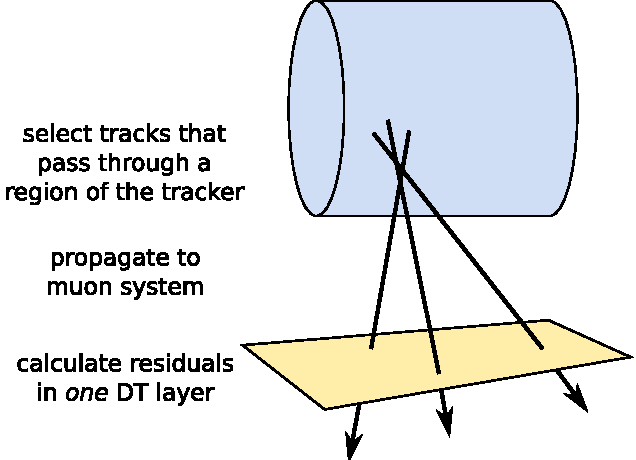
\includegraphics[width=\linewidth]{method.pdf}

\column{0.4\linewidth}
\begin{itemize}
\item Tracker-only fits, propagate to muon system
\item Tracker hits $\ge$ 5
\item Tracker $\chi^2/\mbox{ndf} < 20$
\item Exactly 12 hits on DT segment in wheel~0, station~1, sector~10
\item Look at $x$ residuals on layer~2 of this chamber \\ (arbitrarily chosen)
\item Segment $\chi^2/\mbox{ndf} < 20$
\end{itemize}
\end{columns}

\begin{itemize}
\item Characterize ``a region of the tracker'' by $d_{xy}$, $d_z$, $\phi$, $\cot\theta$, \ldots
\begin{itemize}
\item integrates over a region: only useful for studies of global shape
\end{itemize}

\item In this talk, I only look at $d_{xy}$, $\phi$, and $q/p_T$ (transverse plane)
\end{itemize}
\end{frame}

\begin{frame}
\frametitle{Tracker global distortions}

\begin{itemize}
\item 9 sample modes: \{$R$, $z$, $r\phi$\} displacements vs.\ \{$R$, $z$, $\phi$\}
\item Left: tracker module positions in each mode
\item Right: $\chi^2$ sensitivity of each mode
\end{itemize}

\vspace{-0.5 cm}
\begin{columns}
\column{0.5\linewidth}
\vspace{0.75 cm}
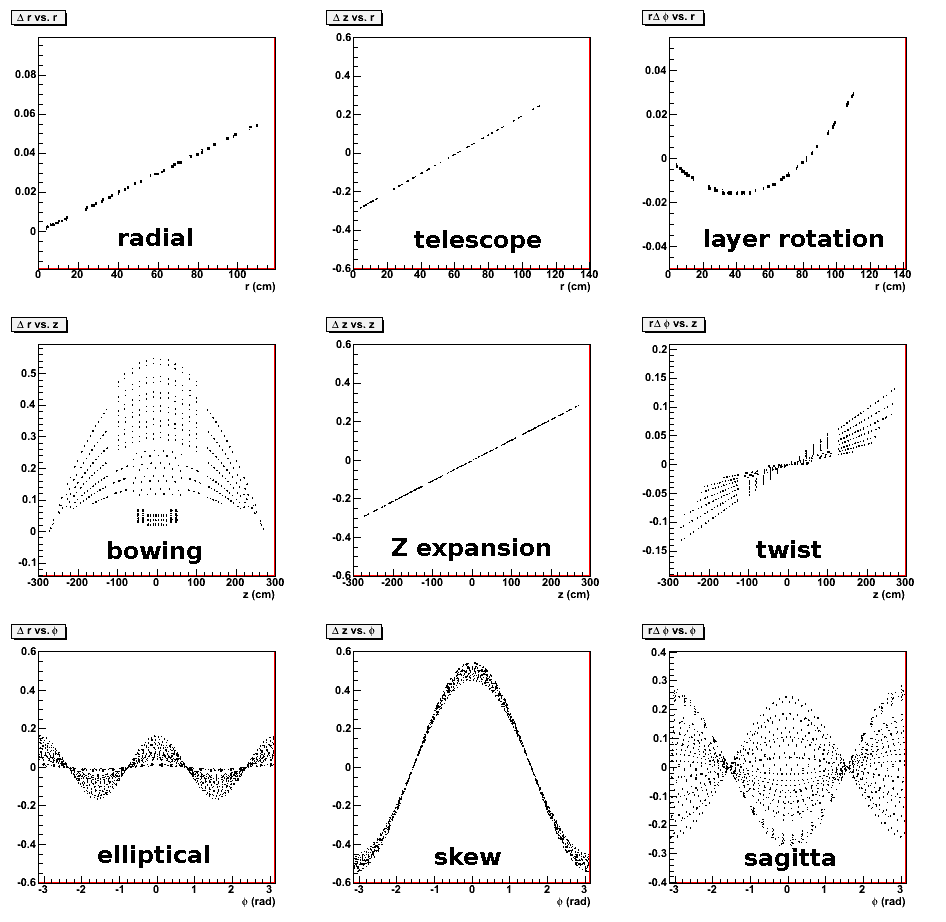
\includegraphics[width=\linewidth]{TrackerSystematics.png}
\column{0.5\linewidth}
\begin{itemize}
\item \textcolor{blue}{Blue:} sensitivity to distortion \textcolor{red}{Red:} recovery \mbox{(may be outdated)\hspace{-1 cm}}
\item Cosmic rays are less sensitive to sagitta than layerRotation
\end{itemize}

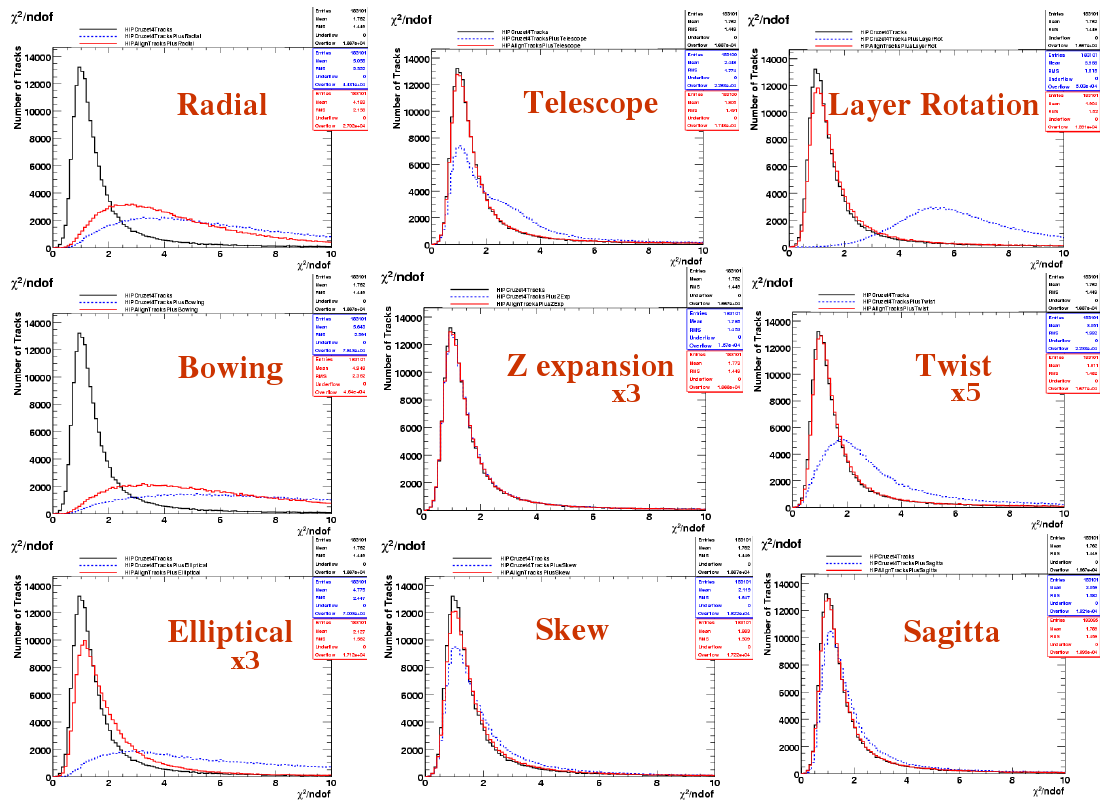
\includegraphics[width=\linewidth]{chi2_sensitivity.png}
\end{columns}

\hfill \textcolor{darkblue}{\scriptsize Zijin Guo Nov 13, 2008}
\end{frame}

\begin{frame}
\frametitle{Evidence for an effect}

\begin{itemize}
\item DT $x$ residuals depend $\sim$symmetrically on $q/p_T$: not a $\vec{B}(\vec{x})$ error
\item MuonPOG May 11, 2009: reasoned from geometry that it could be
  layerRotation (``curl''), but this was ruled out by tracker $\chi^2$

{\tt \tiny http://indico.cern.ch/contributionDisplay.py?contribId=3\&confId=55713}
\end{itemize}

\begin{columns}
\column{0.6\linewidth}
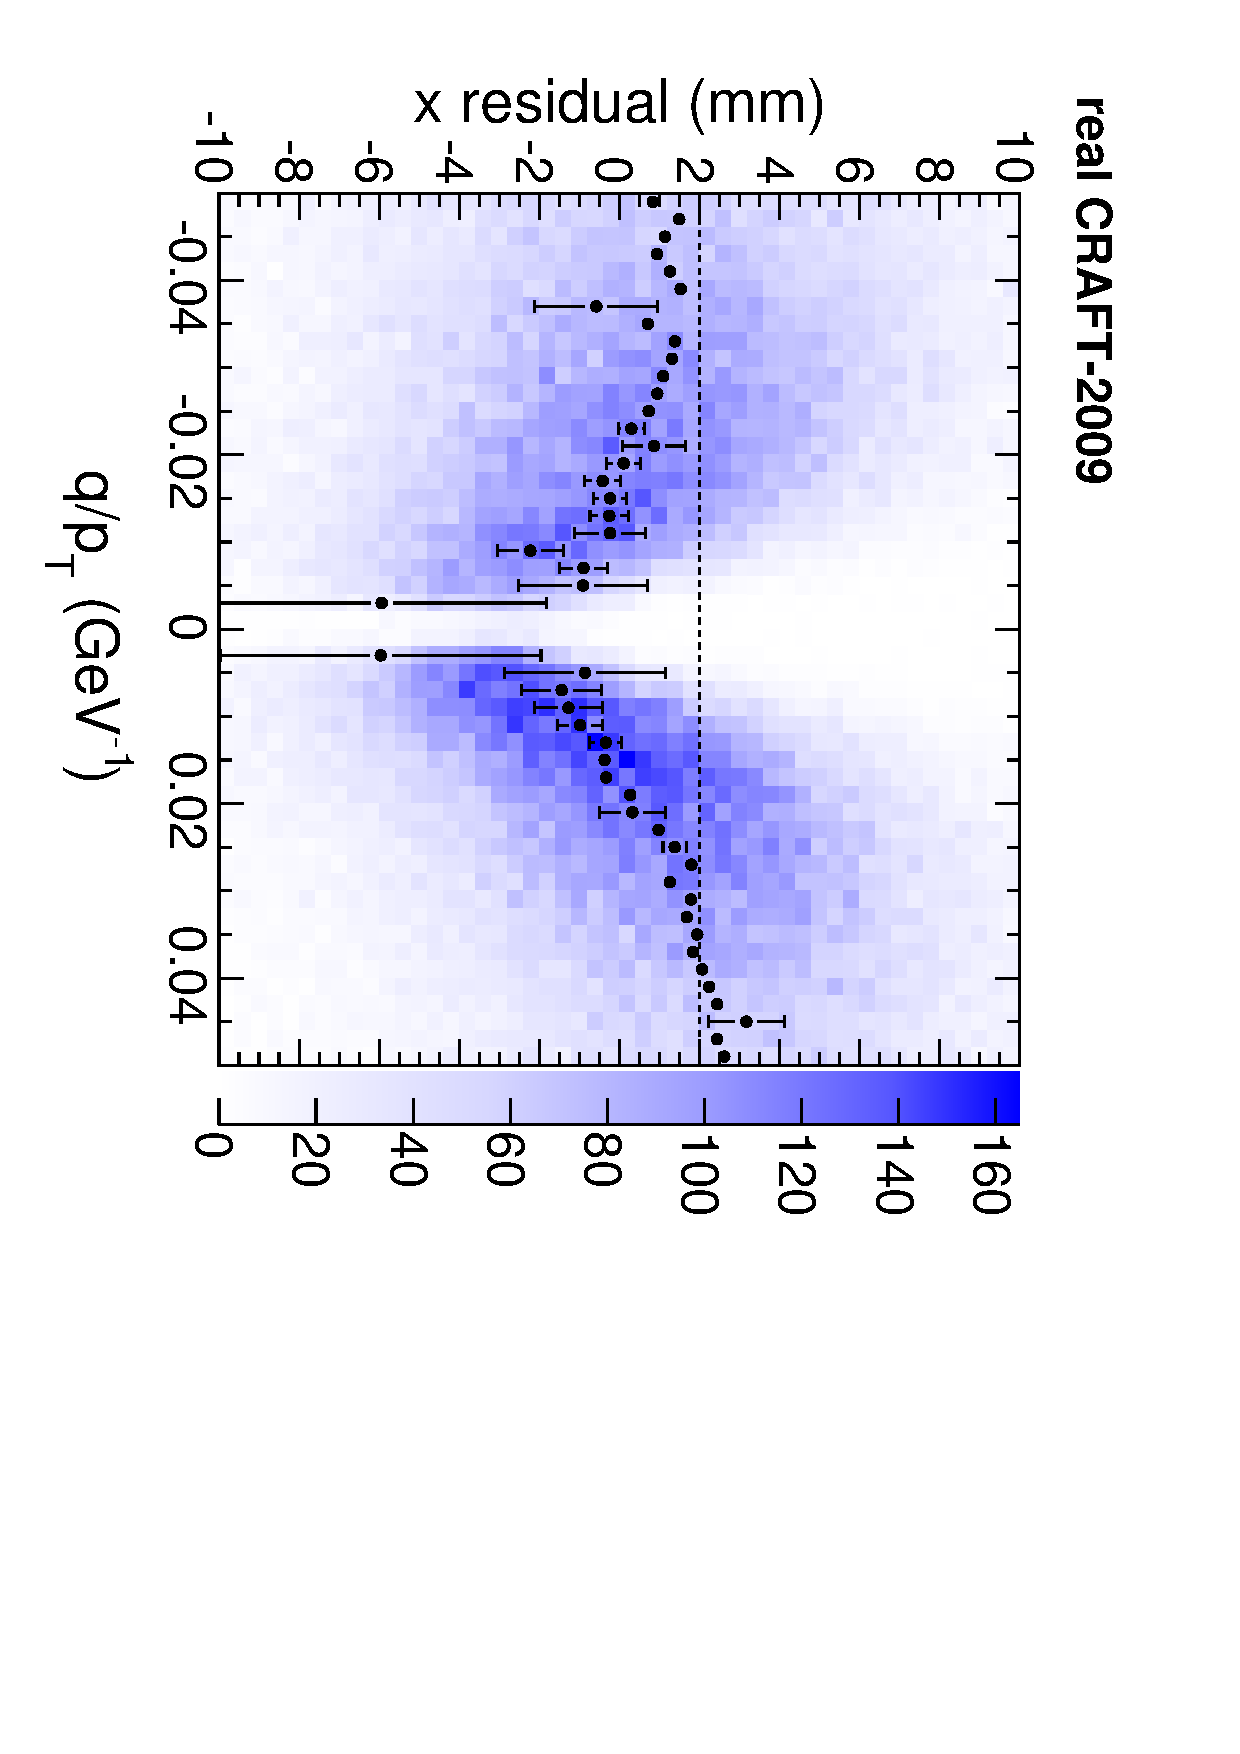
\includegraphics[height=0.49\linewidth, angle=90]{residx-qoverpt_real.pdf}
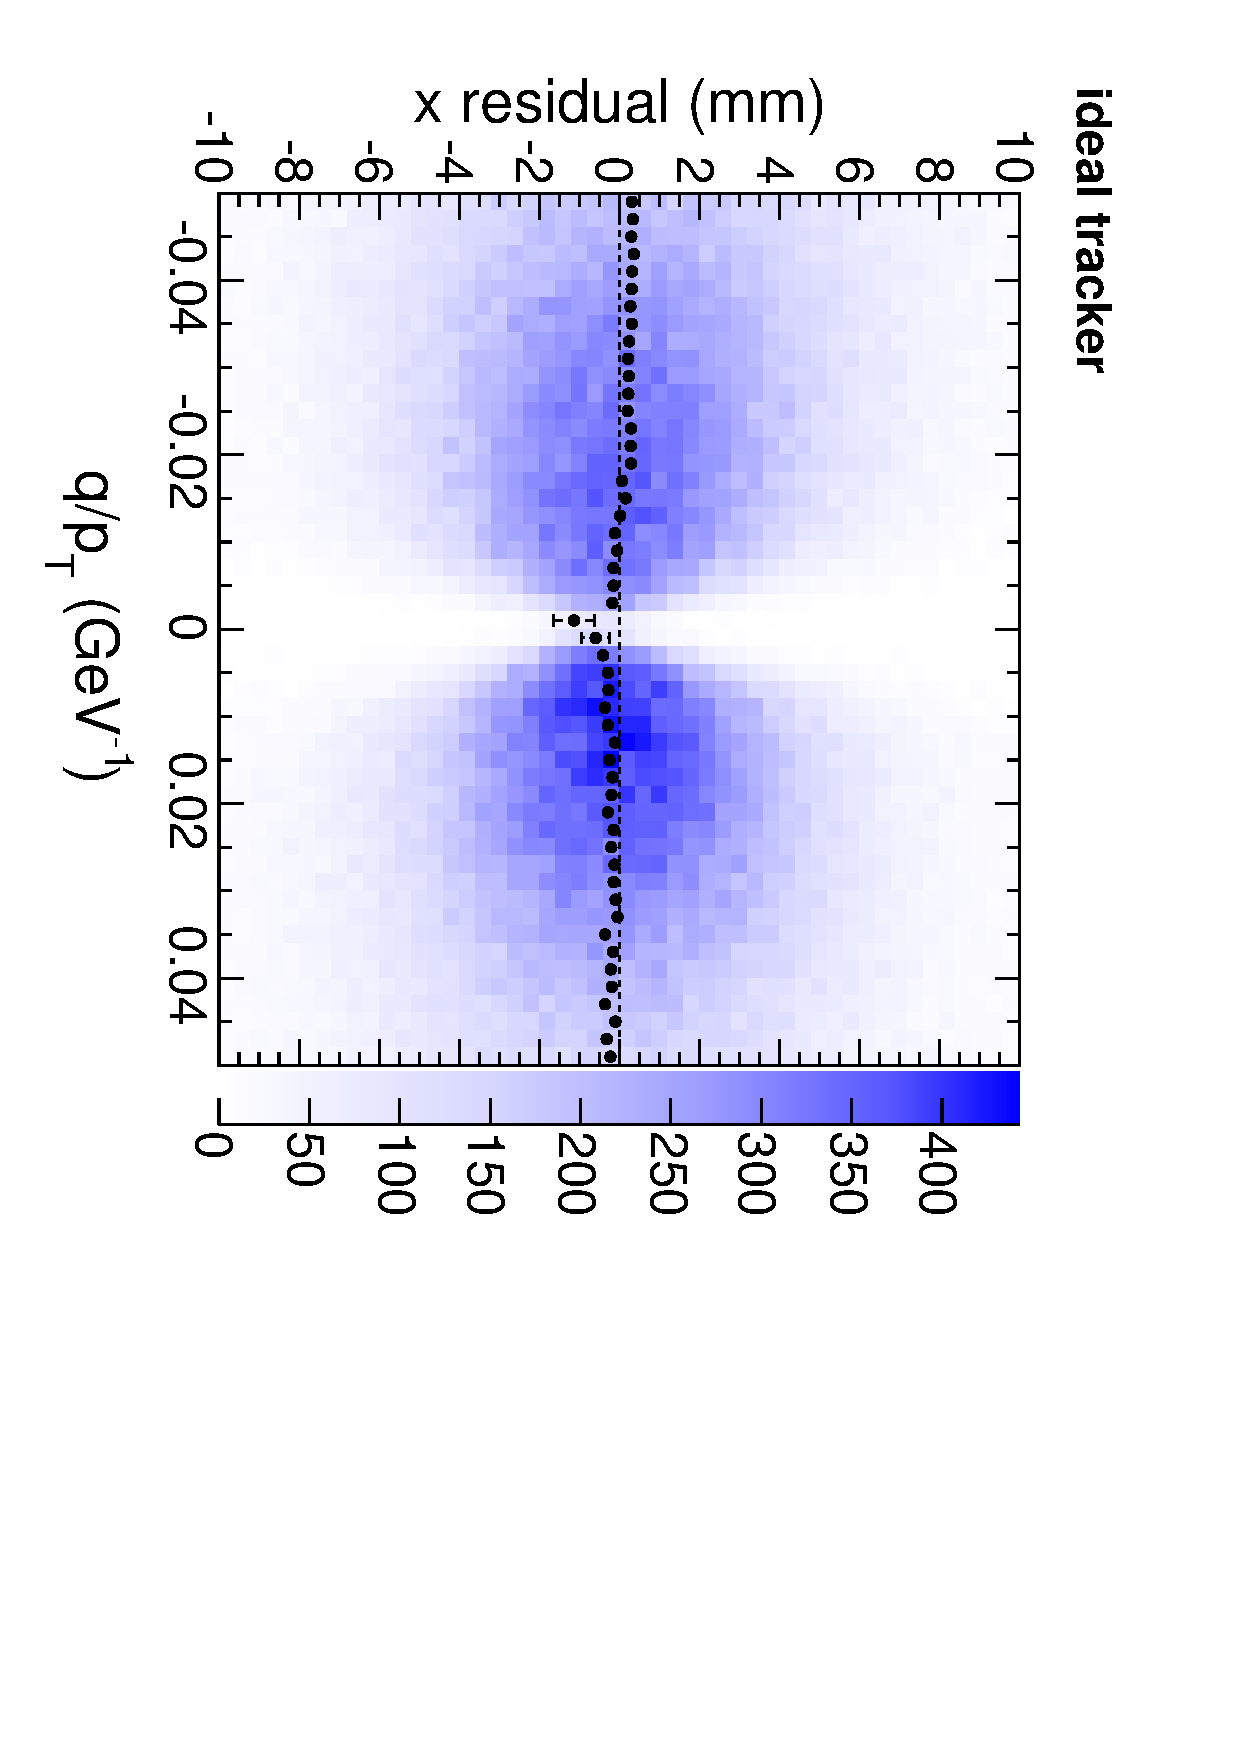
\includegraphics[height=0.49\linewidth, angle=90]{residx-qoverpt_ideal.pdf}

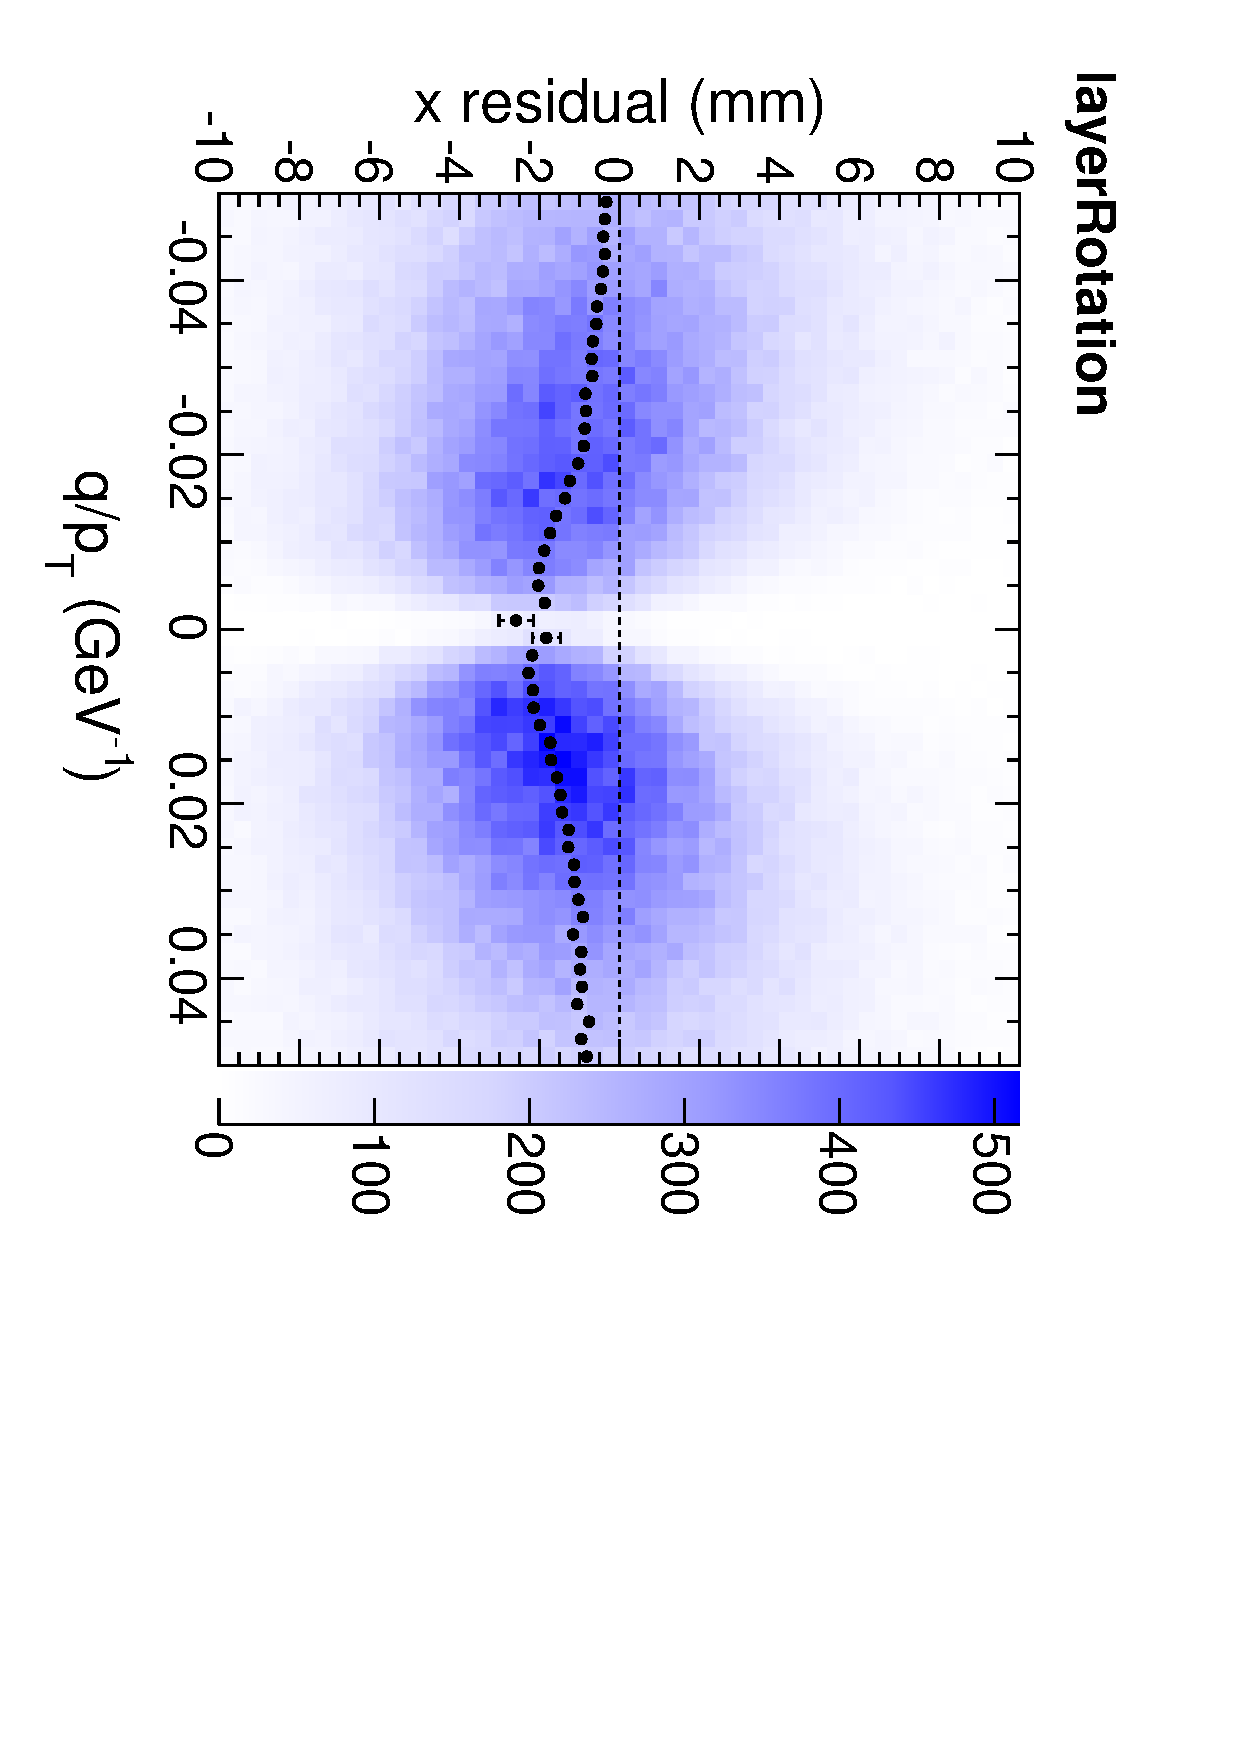
\includegraphics[height=0.49\linewidth, angle=90]{residx-qoverpt_layerRotation.pdf}
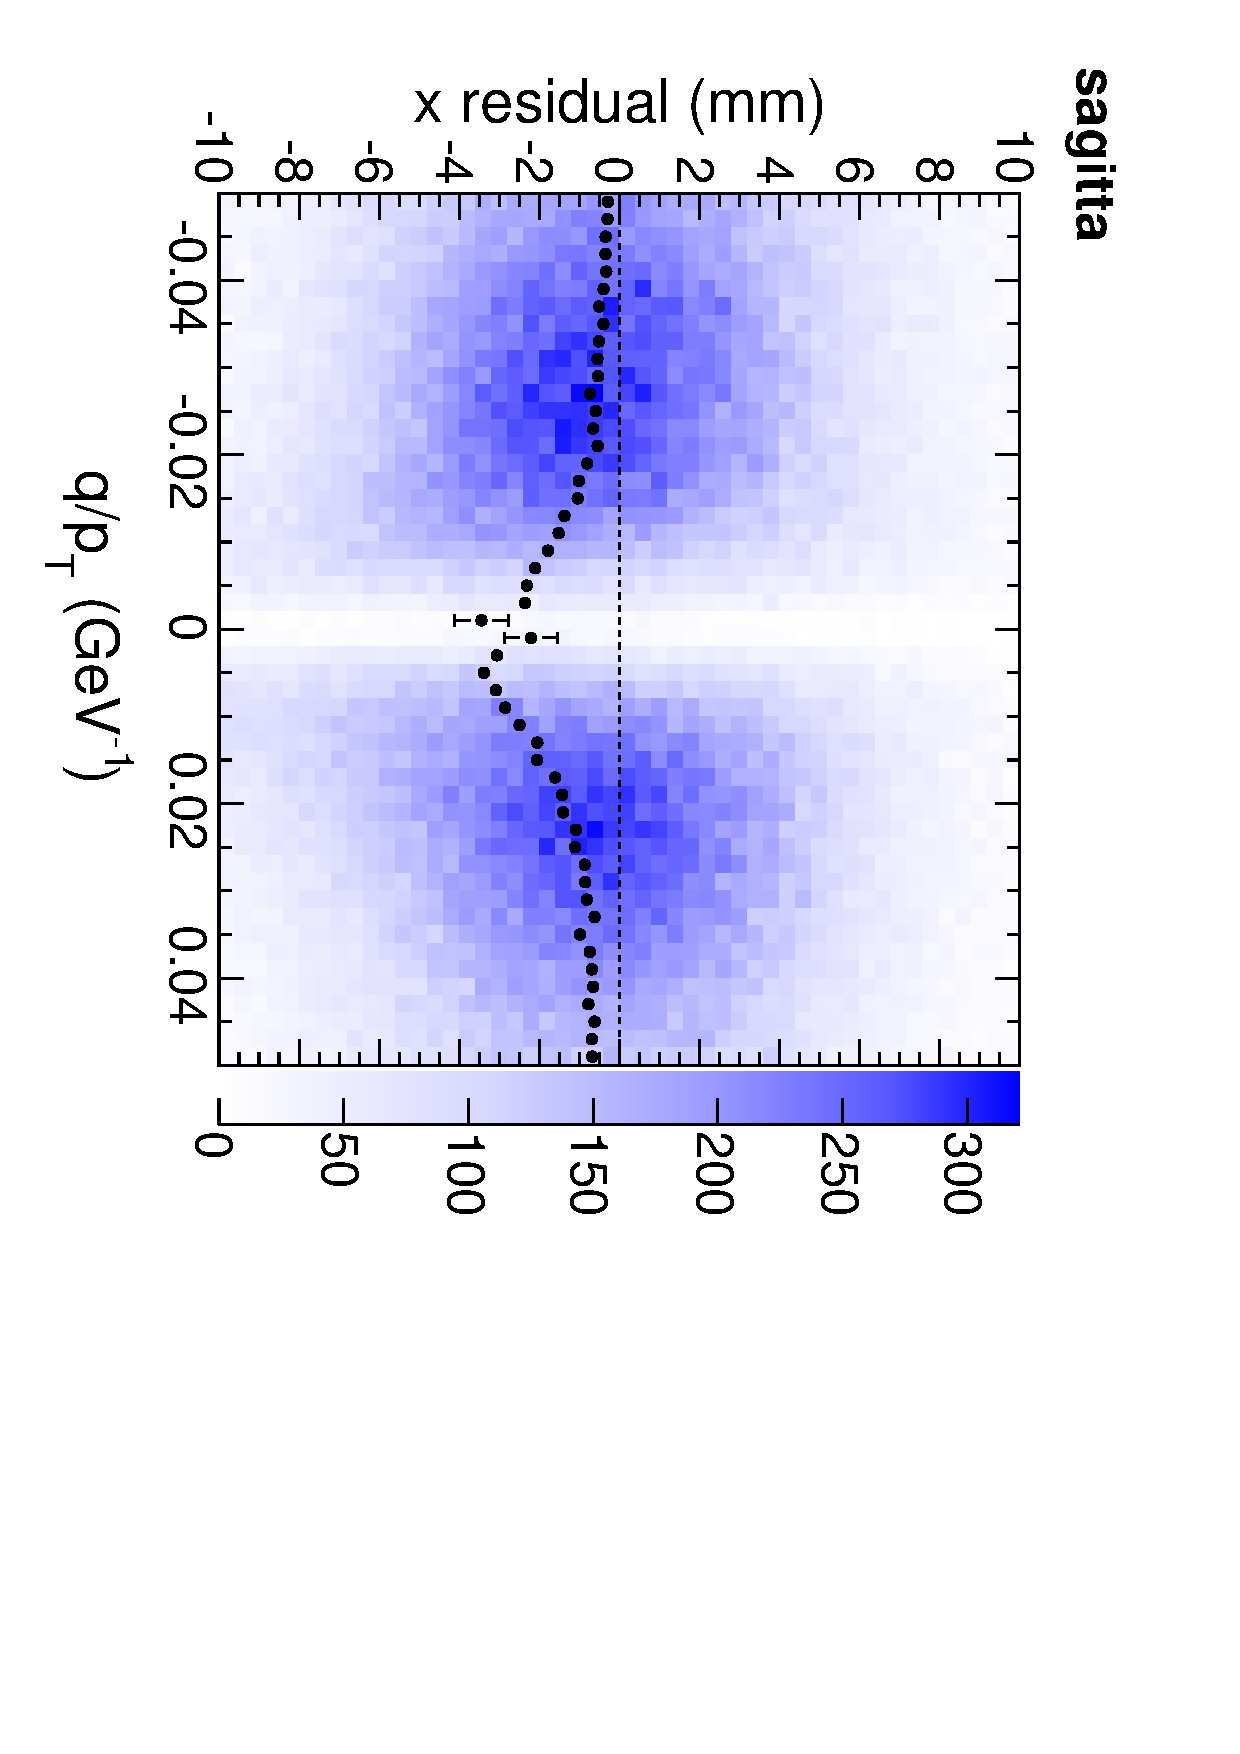
\includegraphics[height=0.49\linewidth, angle=90]{residx-qoverpt_sagitta.pdf}

\column{0.3\linewidth}
\mbox{\hspace{-0.75 cm}\begin{minipage}{1.2\linewidth}
\begin{itemize}
\item Top-left: real data, CRAFT-2009 in 3\_2\_7 with the latest tracker alignment
\item Others: Monte Carlo with different tracker geometries
\item blues: \mbox{2-D distribution\hspace{-1 cm}} \\ of residuals vs.~$q/p_T$
\item black points: profile \mbox{(vertical mean by bin)\hspace{-1 cm}}
\end{itemize}
\end{minipage}}
\end{columns}
\end{frame}

\begin{frame}
\frametitle{Residual vs.~$d_{xy}$ and $q/p_T$}

\begin{itemize}
\item Try to get a global picture with 2-D profiles
\item Color scale is mean $x$ residual (mm) in each 2-D bin
\item Not one of the 9 sample modes has exactly the same shape as data
\end{itemize}

\begin{columns}
\column{0.4\linewidth}
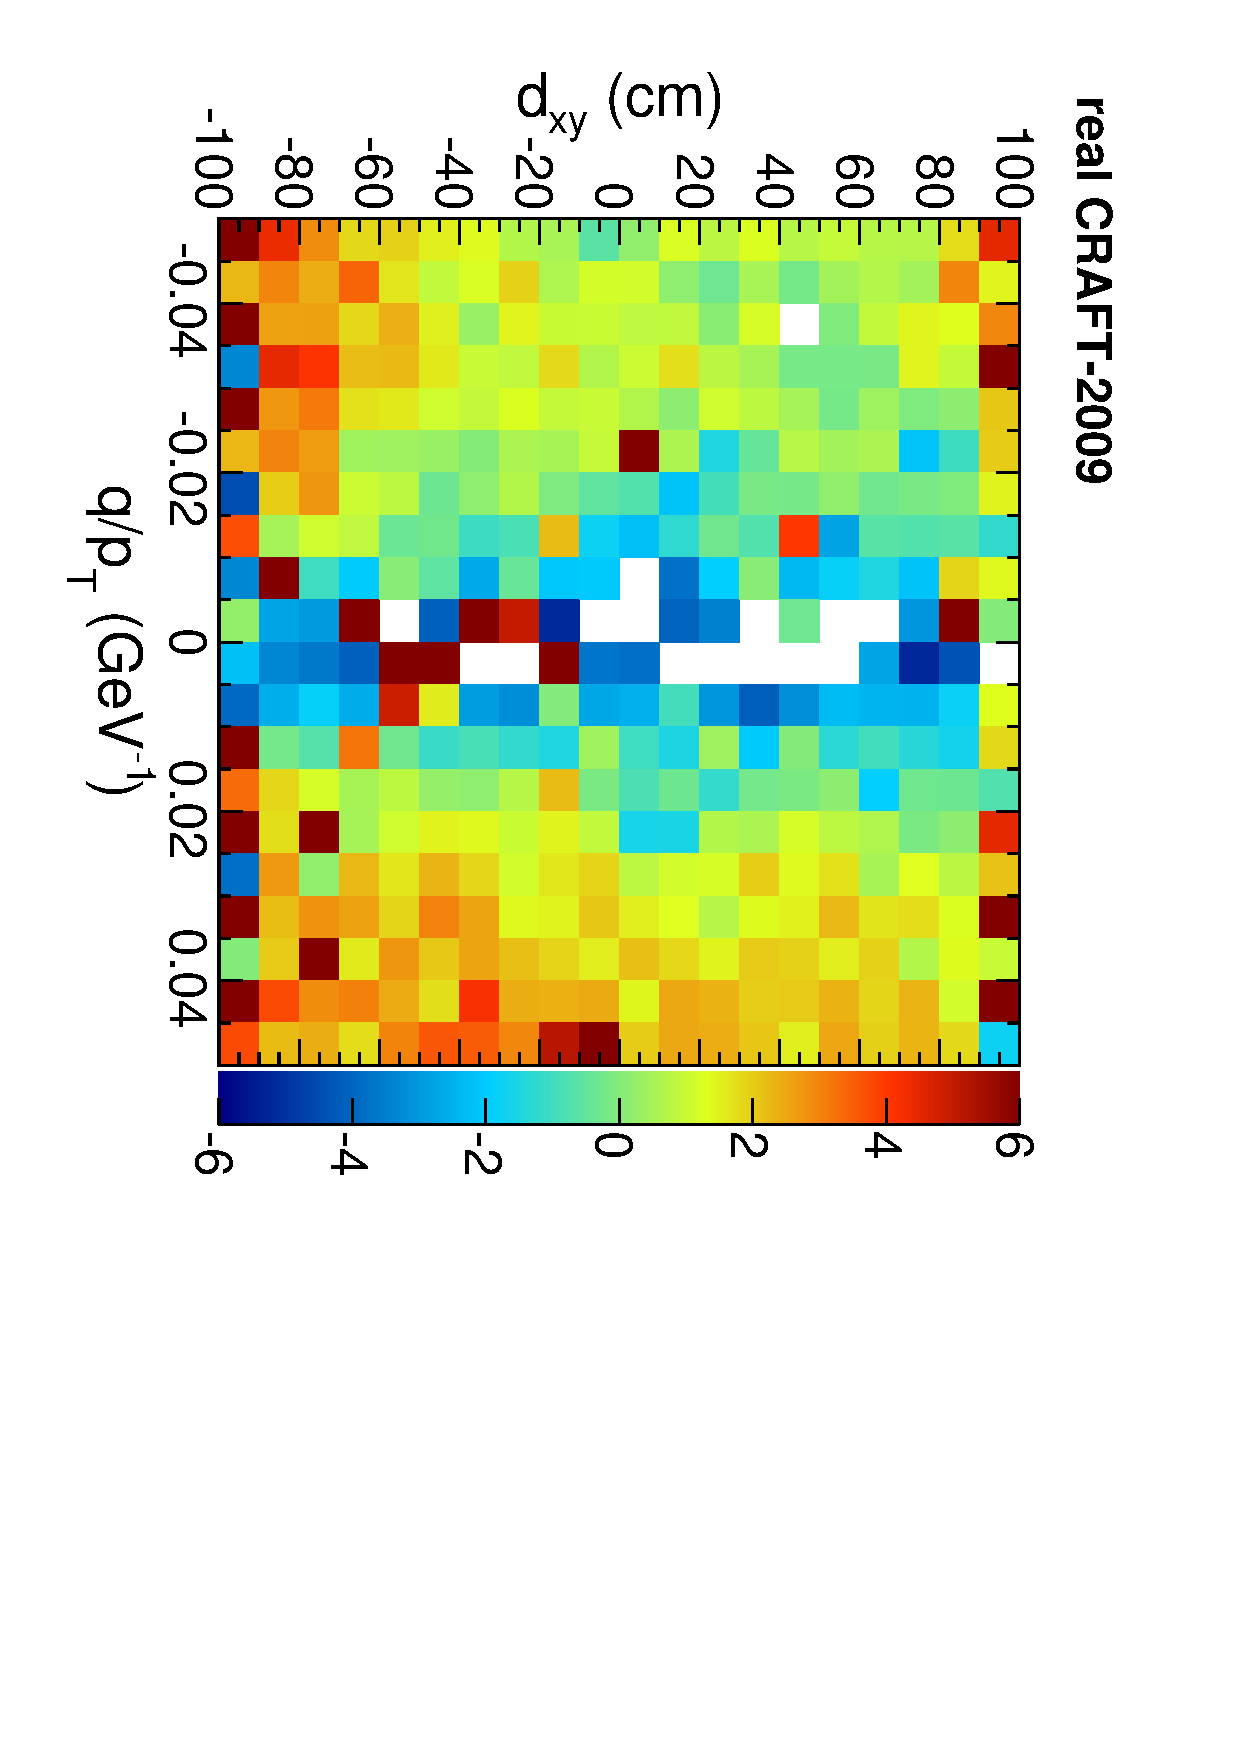
\includegraphics[height=\linewidth, angle=90]{residx-dxy-qoverpt_real.pdf}

\column{0.6\linewidth}
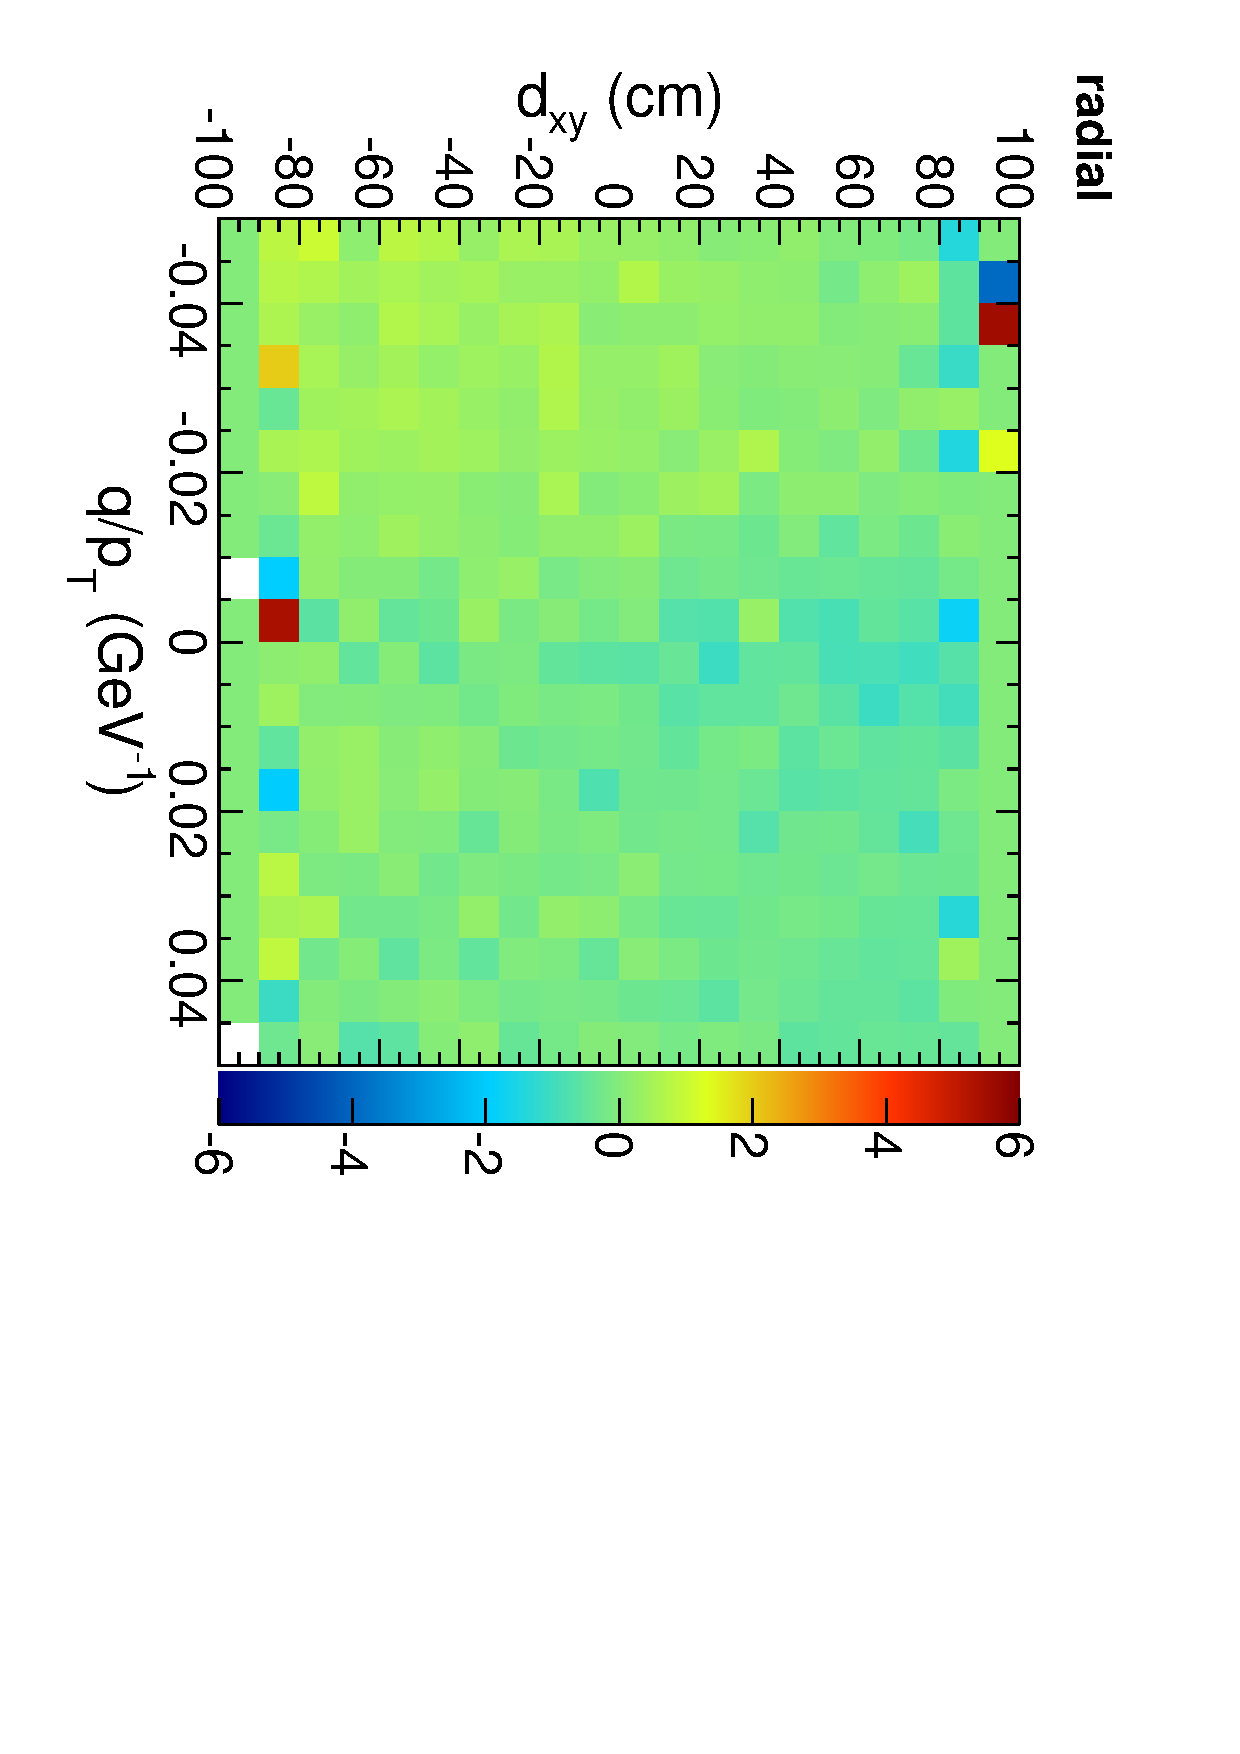
\includegraphics[height=0.32\linewidth, angle=90]{residx-dxy-qoverpt_radial.pdf}
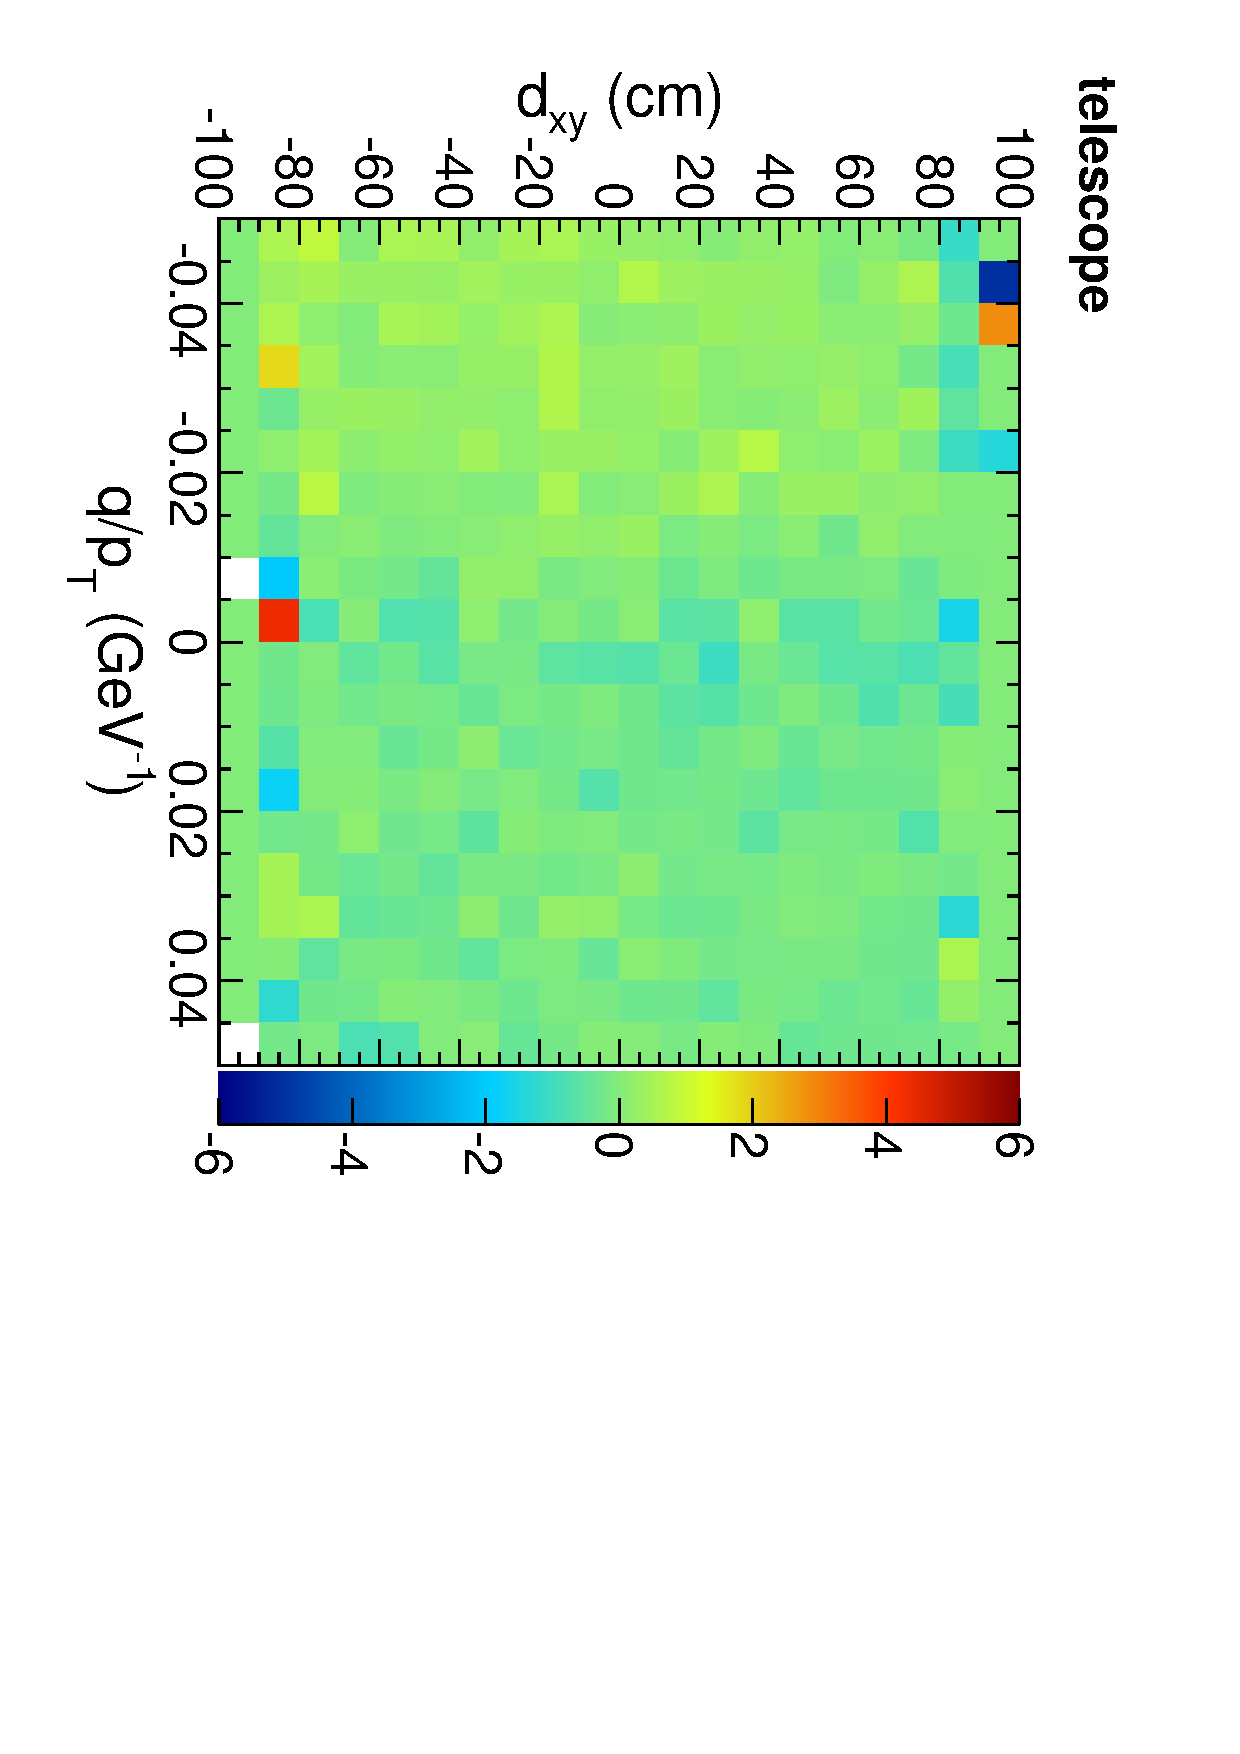
\includegraphics[height=0.32\linewidth, angle=90]{residx-dxy-qoverpt_telescope.pdf}
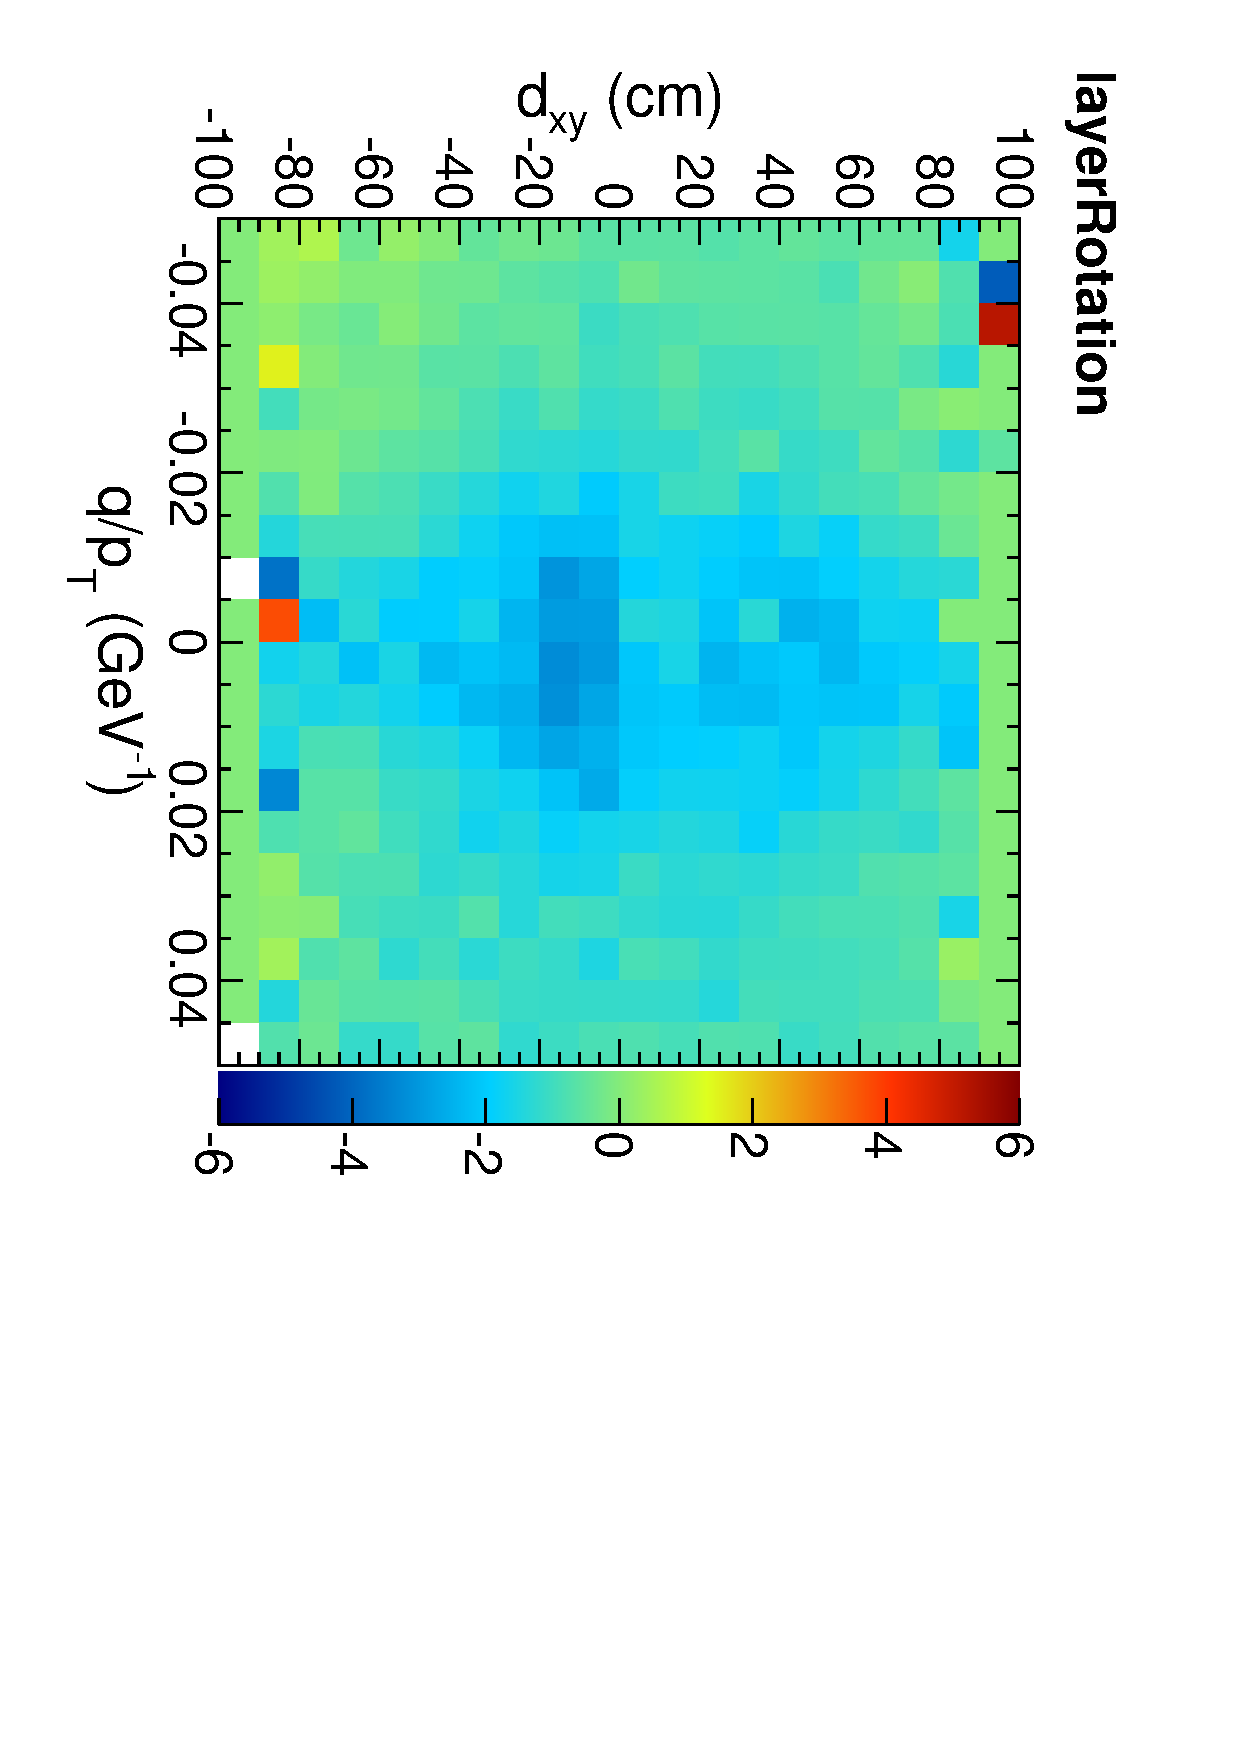
\includegraphics[height=0.32\linewidth, angle=90]{residx-dxy-qoverpt_layerRotation.pdf}

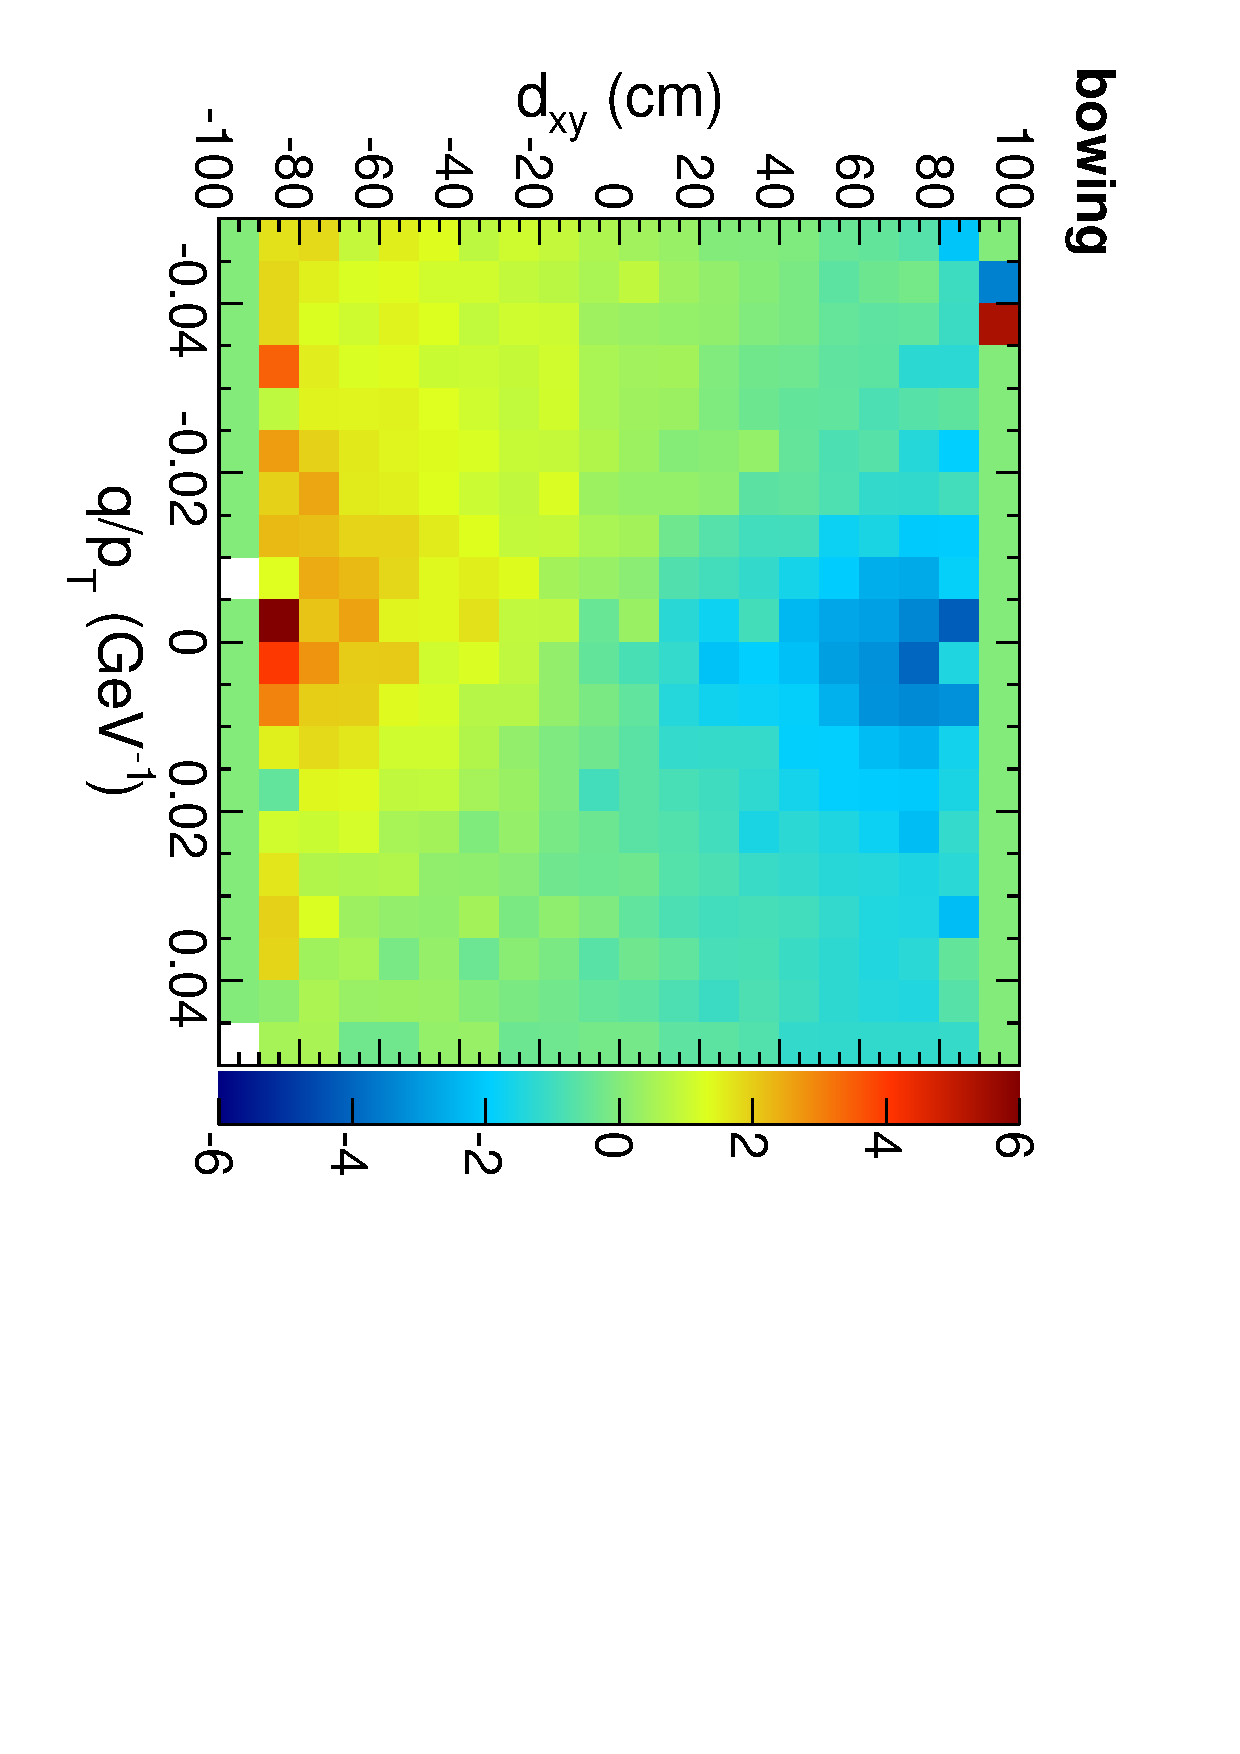
\includegraphics[height=0.32\linewidth, angle=90]{residx-dxy-qoverpt_bowing.pdf}
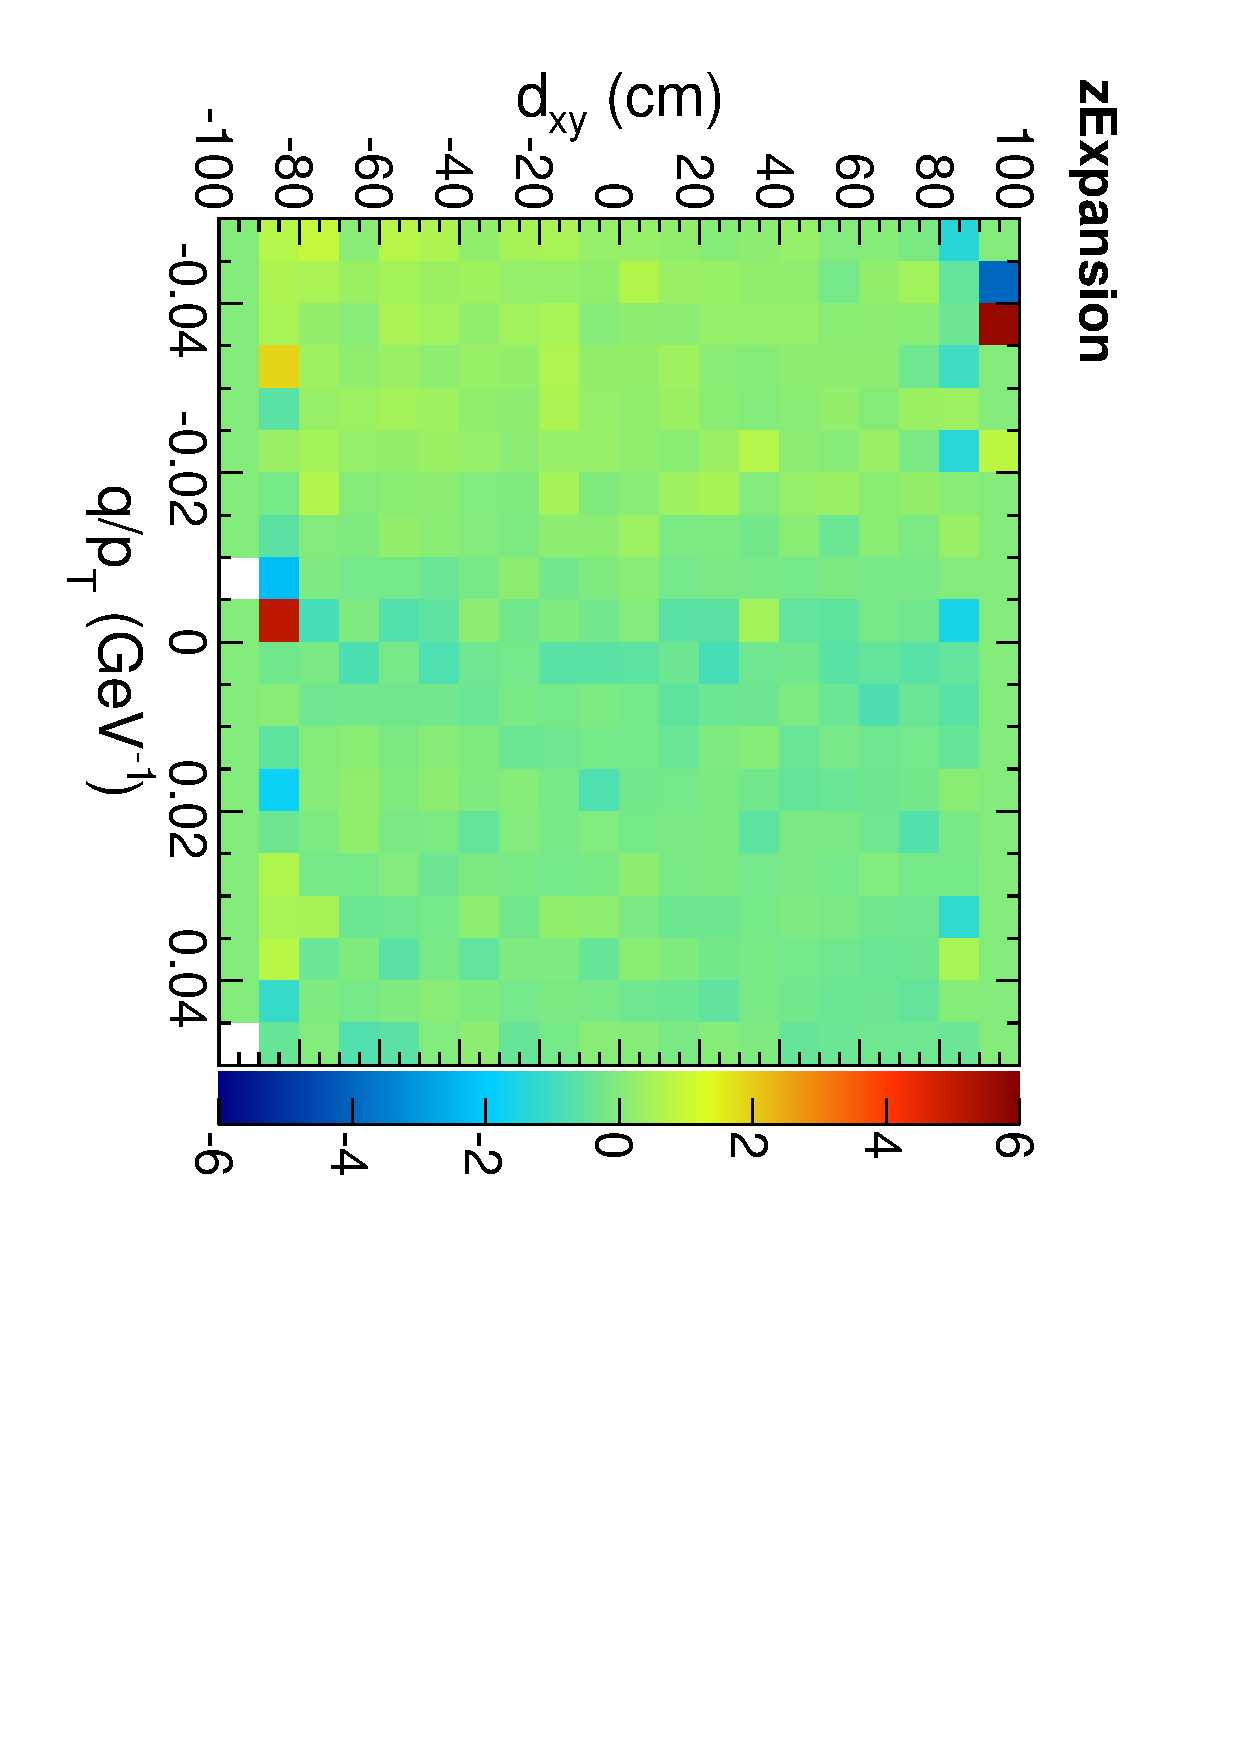
\includegraphics[height=0.32\linewidth, angle=90]{residx-dxy-qoverpt_zExpansion.pdf}
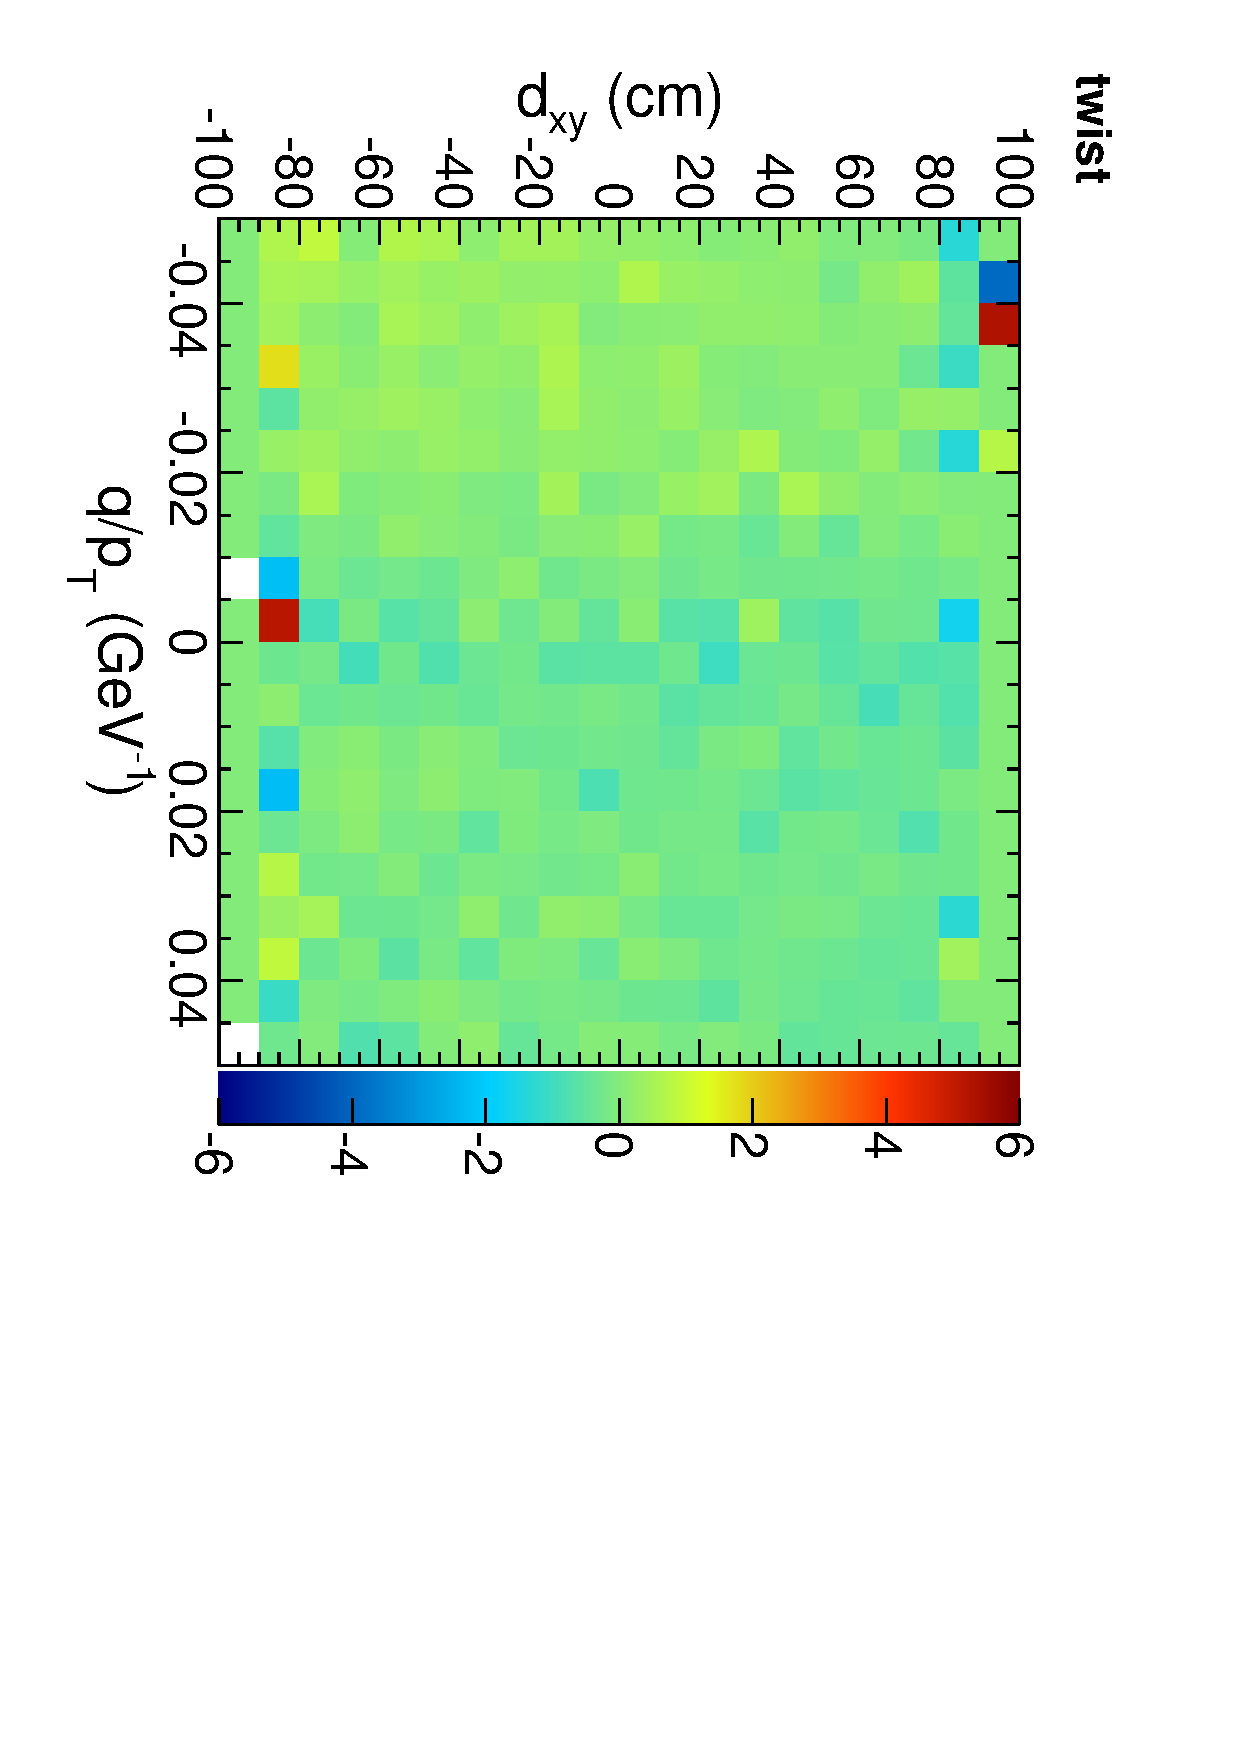
\includegraphics[height=0.32\linewidth, angle=90]{residx-dxy-qoverpt_twist.pdf}

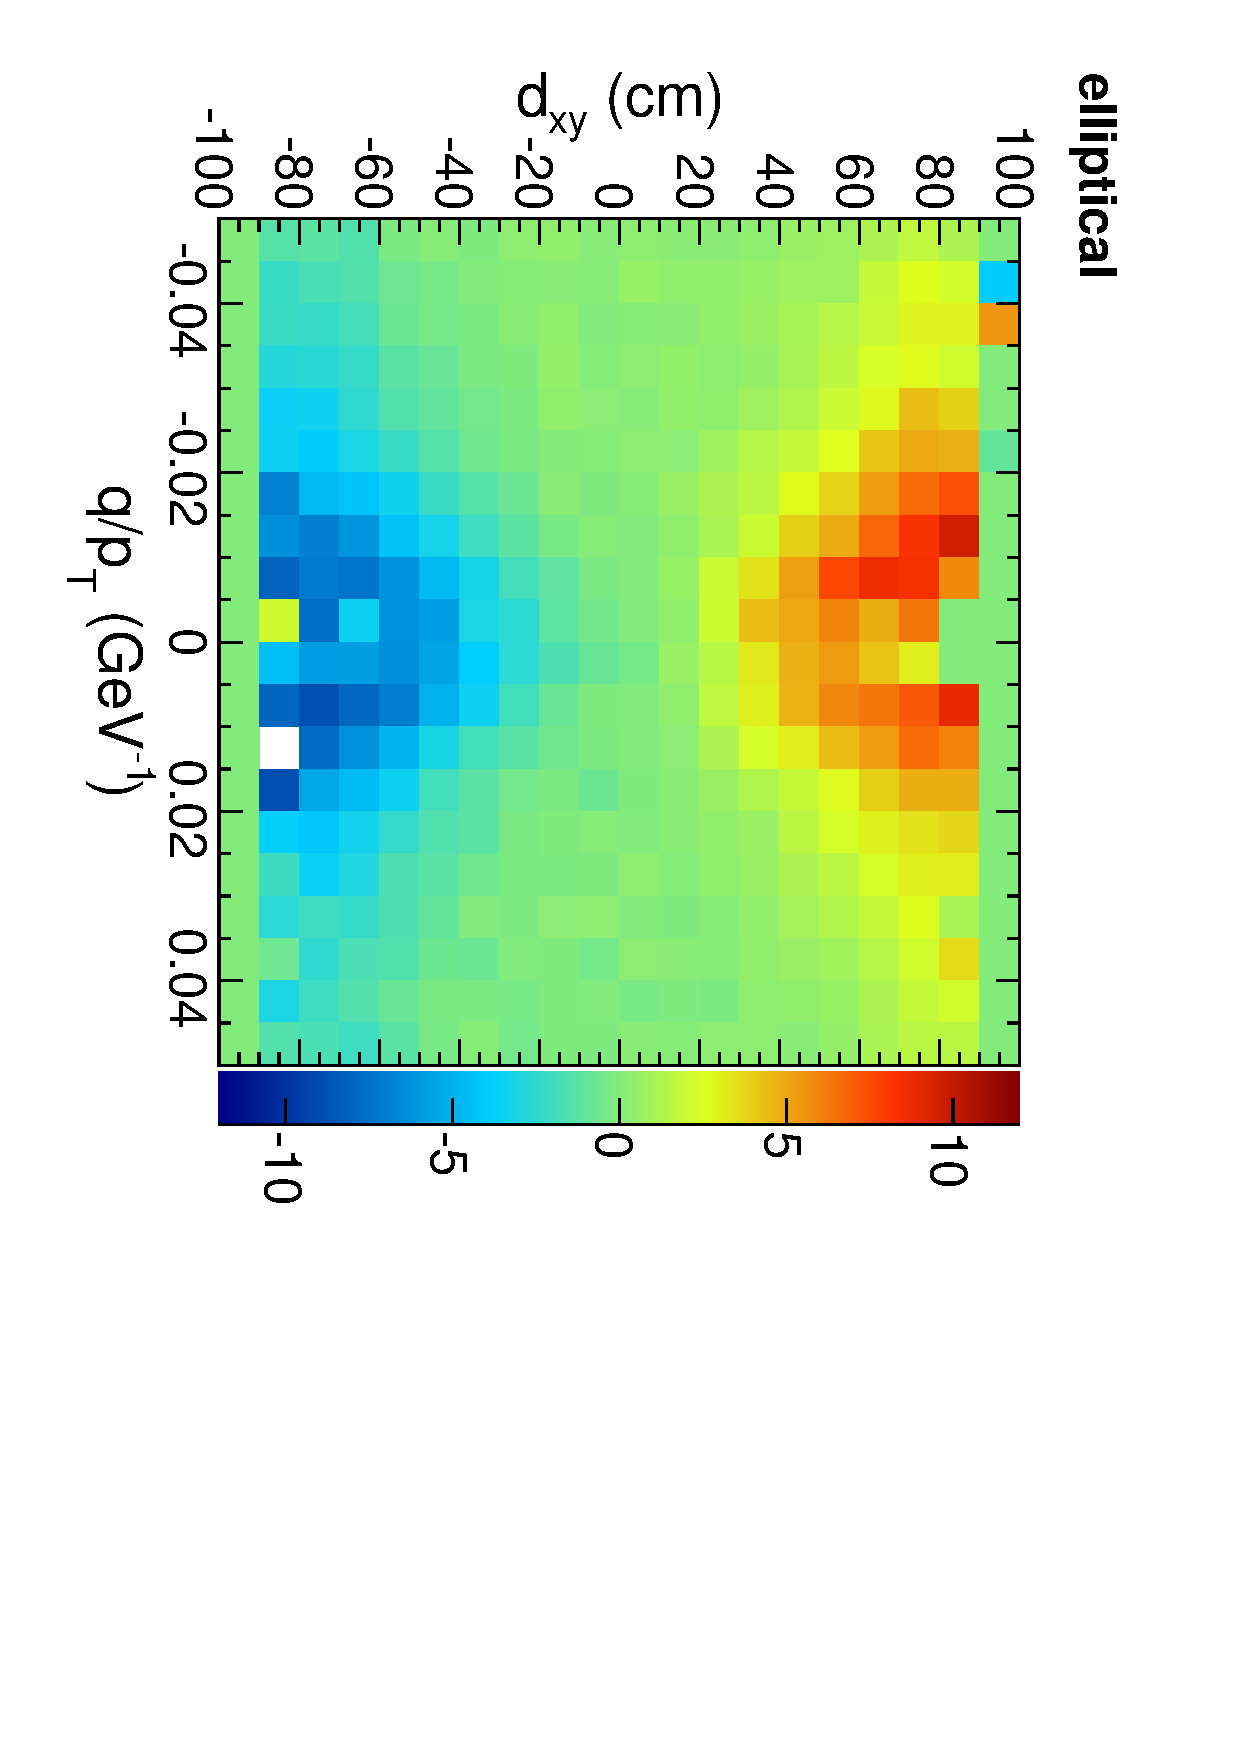
\includegraphics[height=0.32\linewidth, angle=90]{residx-dxy-qoverpt_elliptical.pdf}
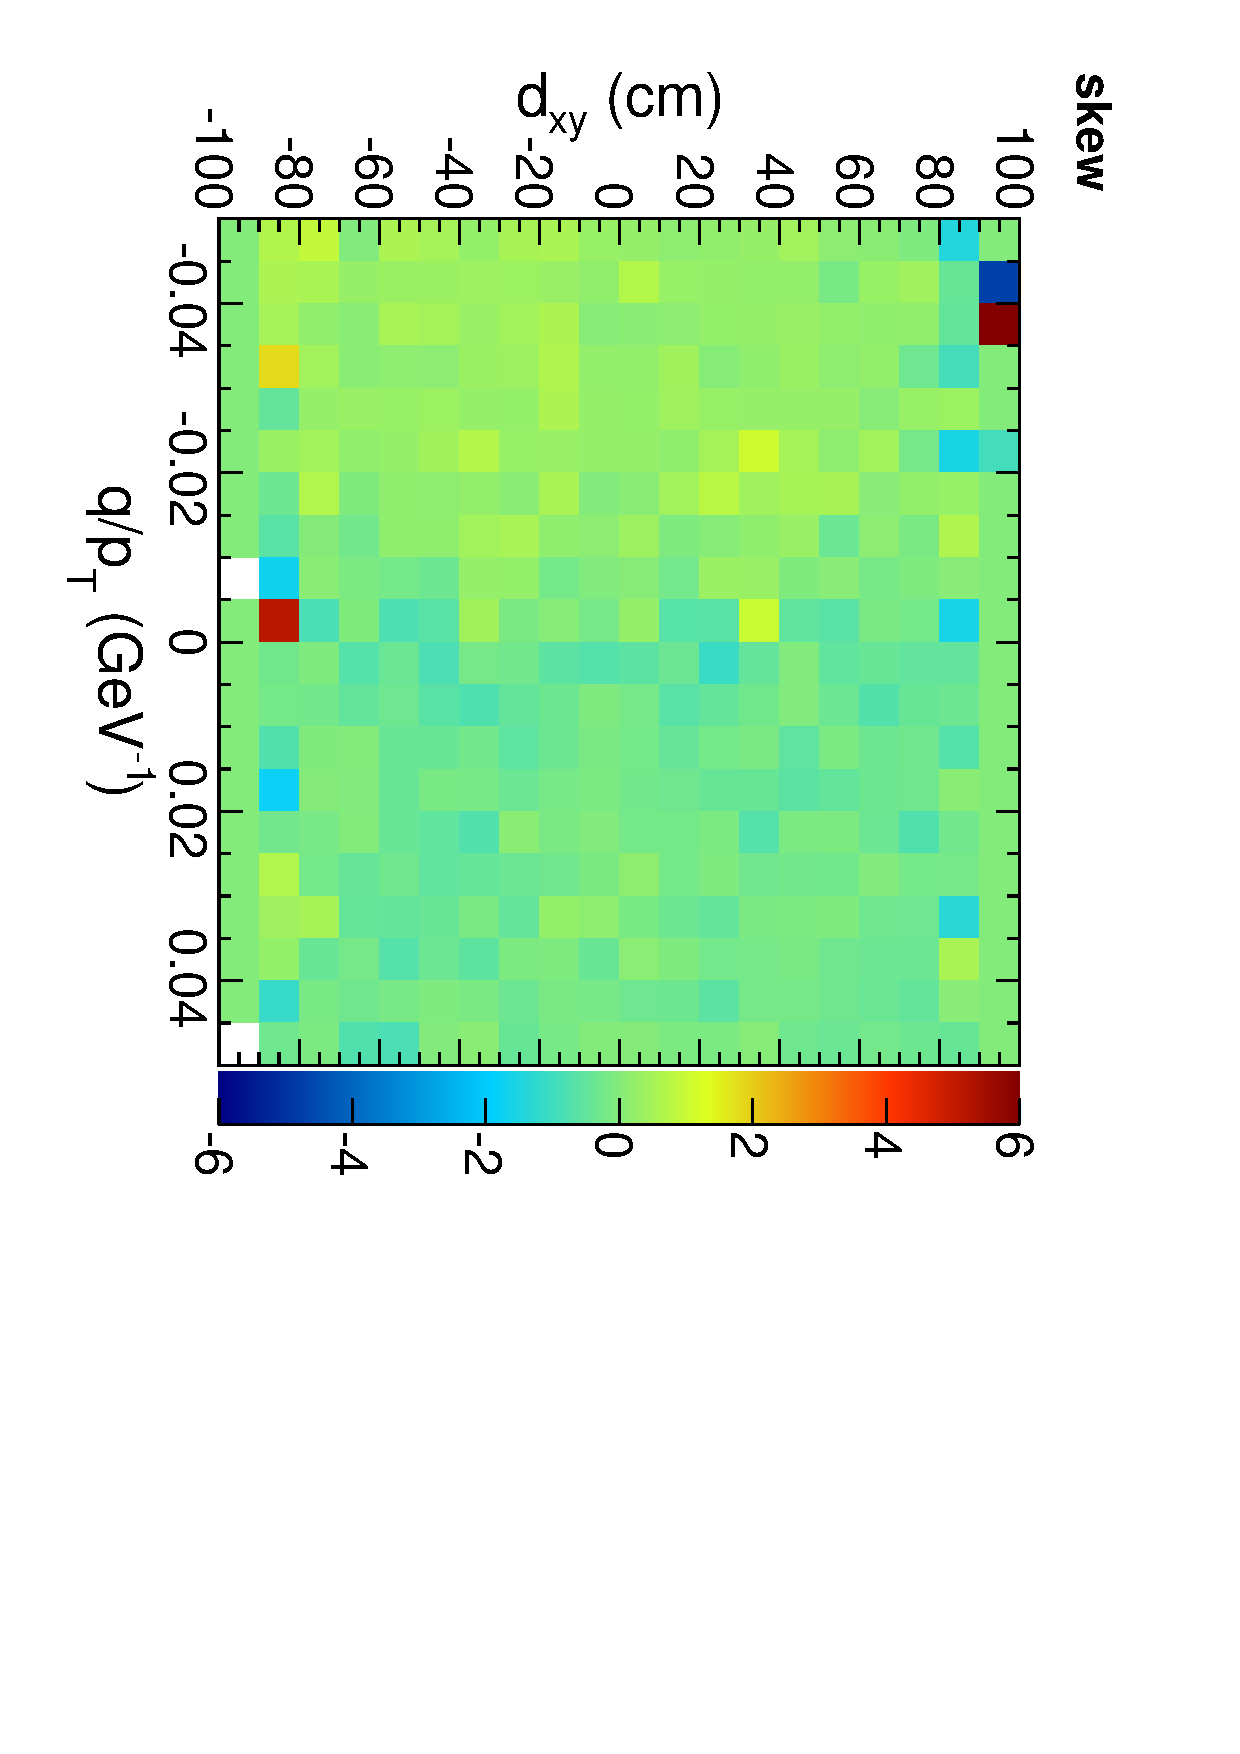
\includegraphics[height=0.32\linewidth, angle=90]{residx-dxy-qoverpt_skew.pdf}
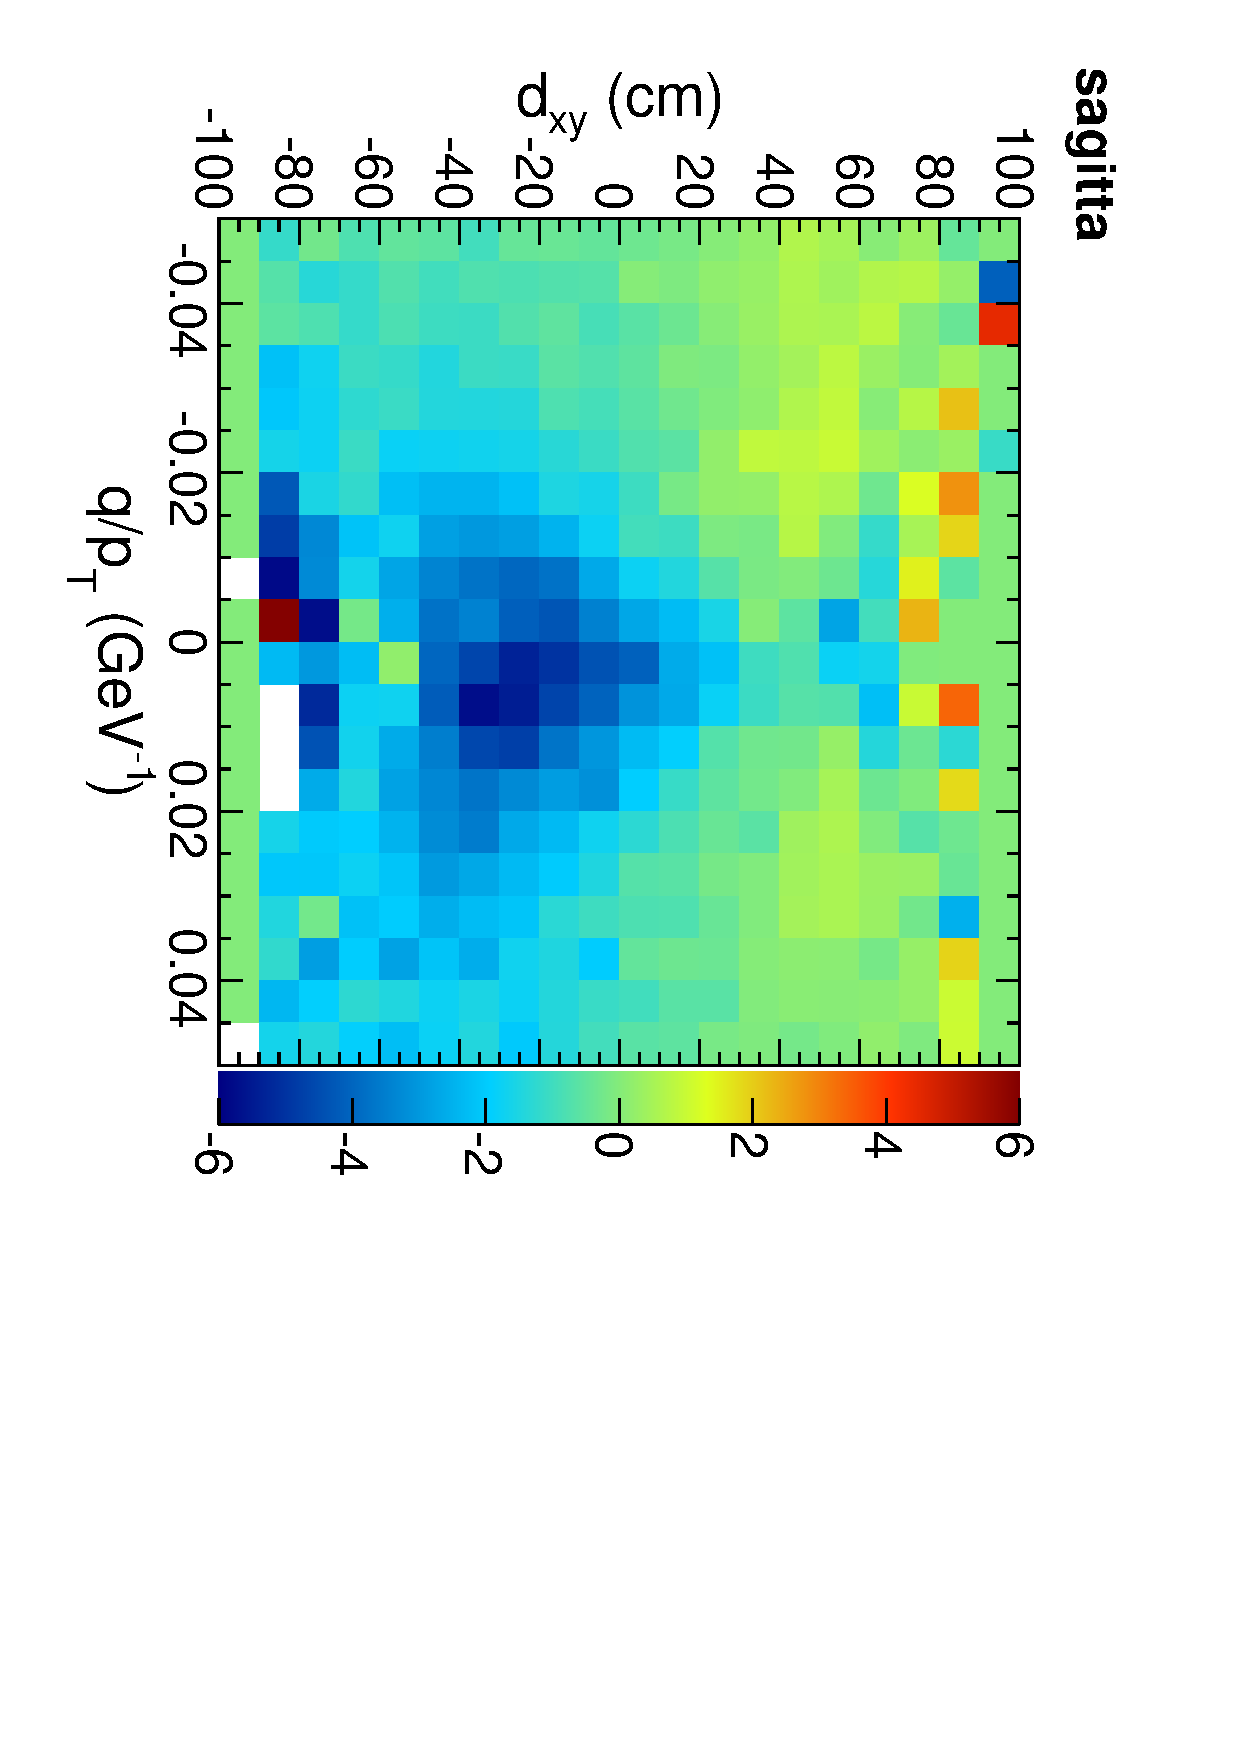
\includegraphics[height=0.32\linewidth, angle=90]{residx-dxy-qoverpt_sagitta.pdf}
\end{columns}
\end{frame}

\begin{frame}
\frametitle{Residual vs.~$\phi$ and $q/p_T$}

\begin{itemize}
\item Try to get a global picture with 2-D profiles
\item Color scale is mean $x$ residual (mm) in each 2-D bin
\item Not one of the 9 sample modes has exactly the same shape as data
\end{itemize}

\begin{columns}
\column{0.4\linewidth}
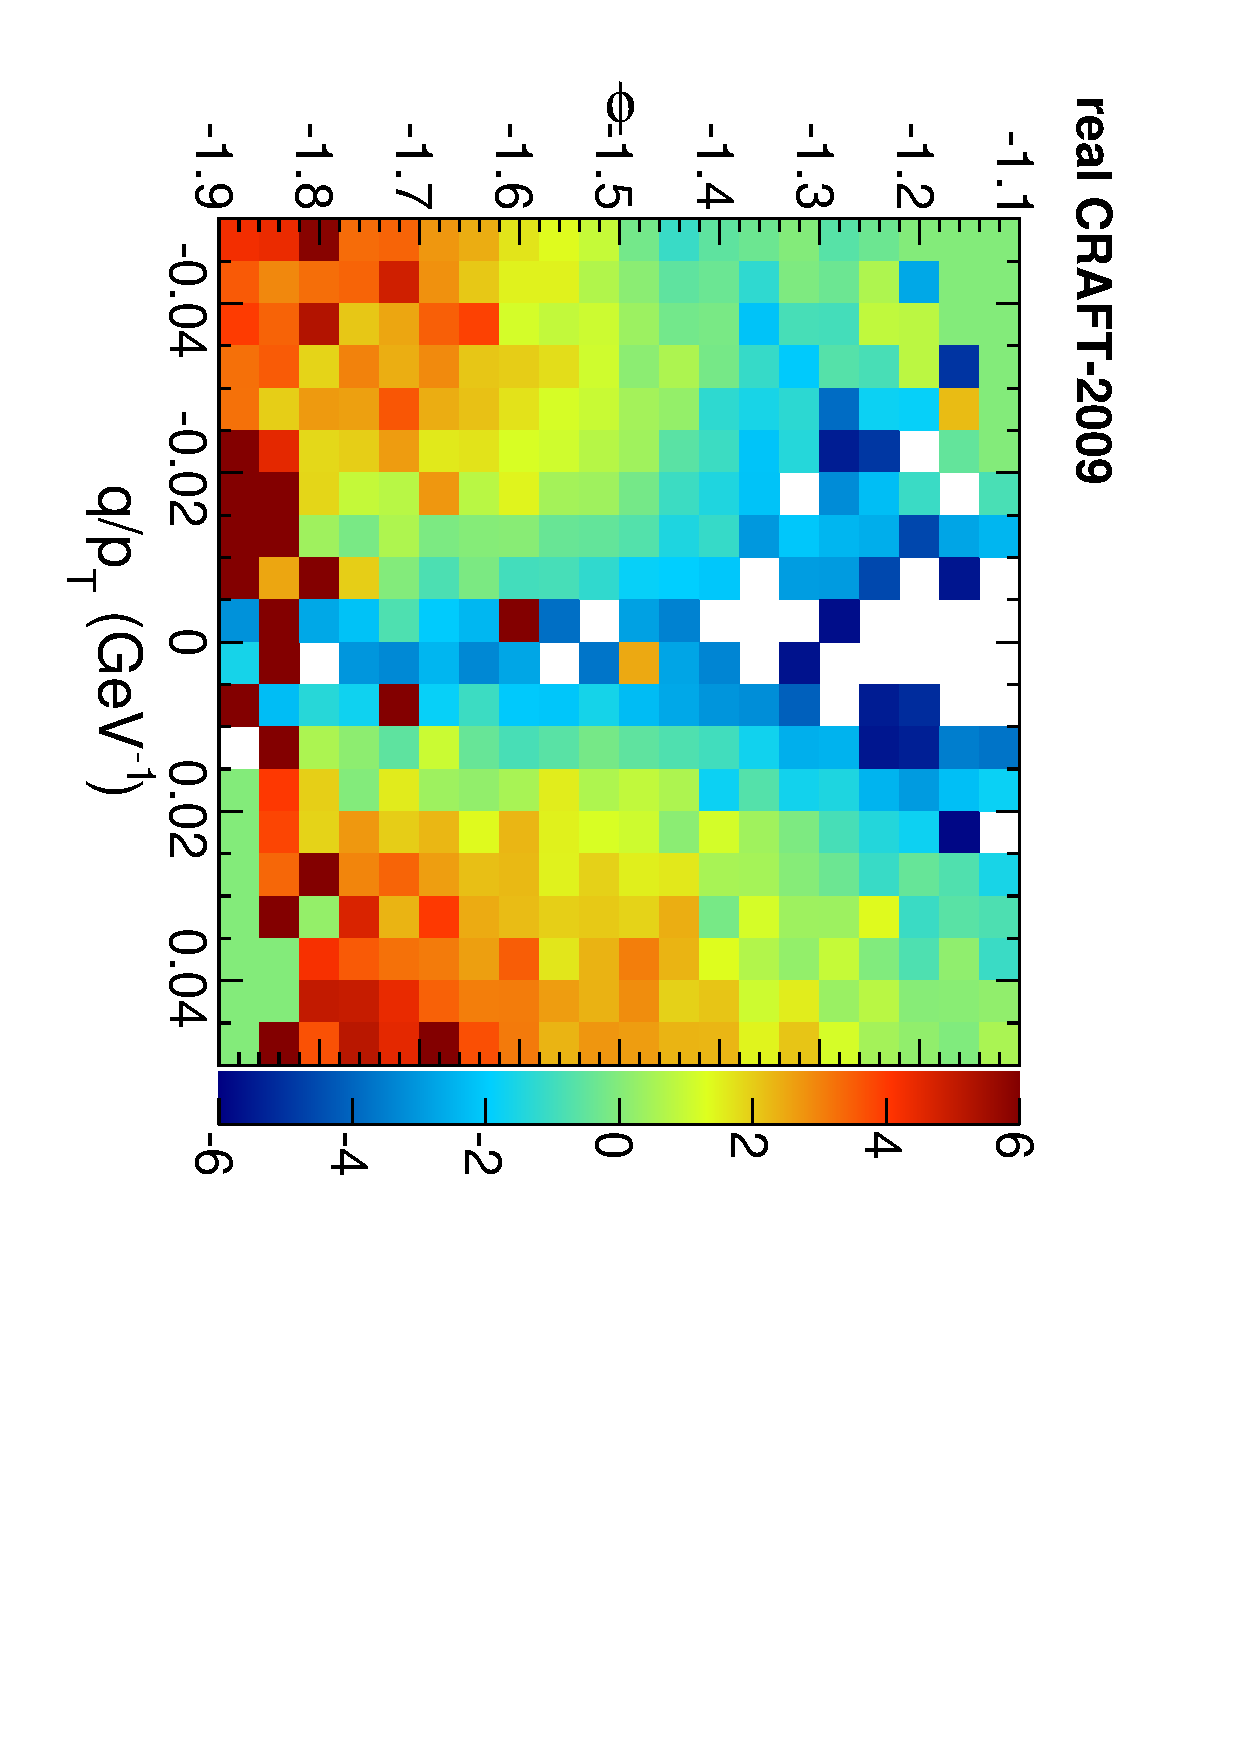
\includegraphics[height=\linewidth, angle=90]{residx-phi-qoverpt_real.pdf}

\column{0.6\linewidth}
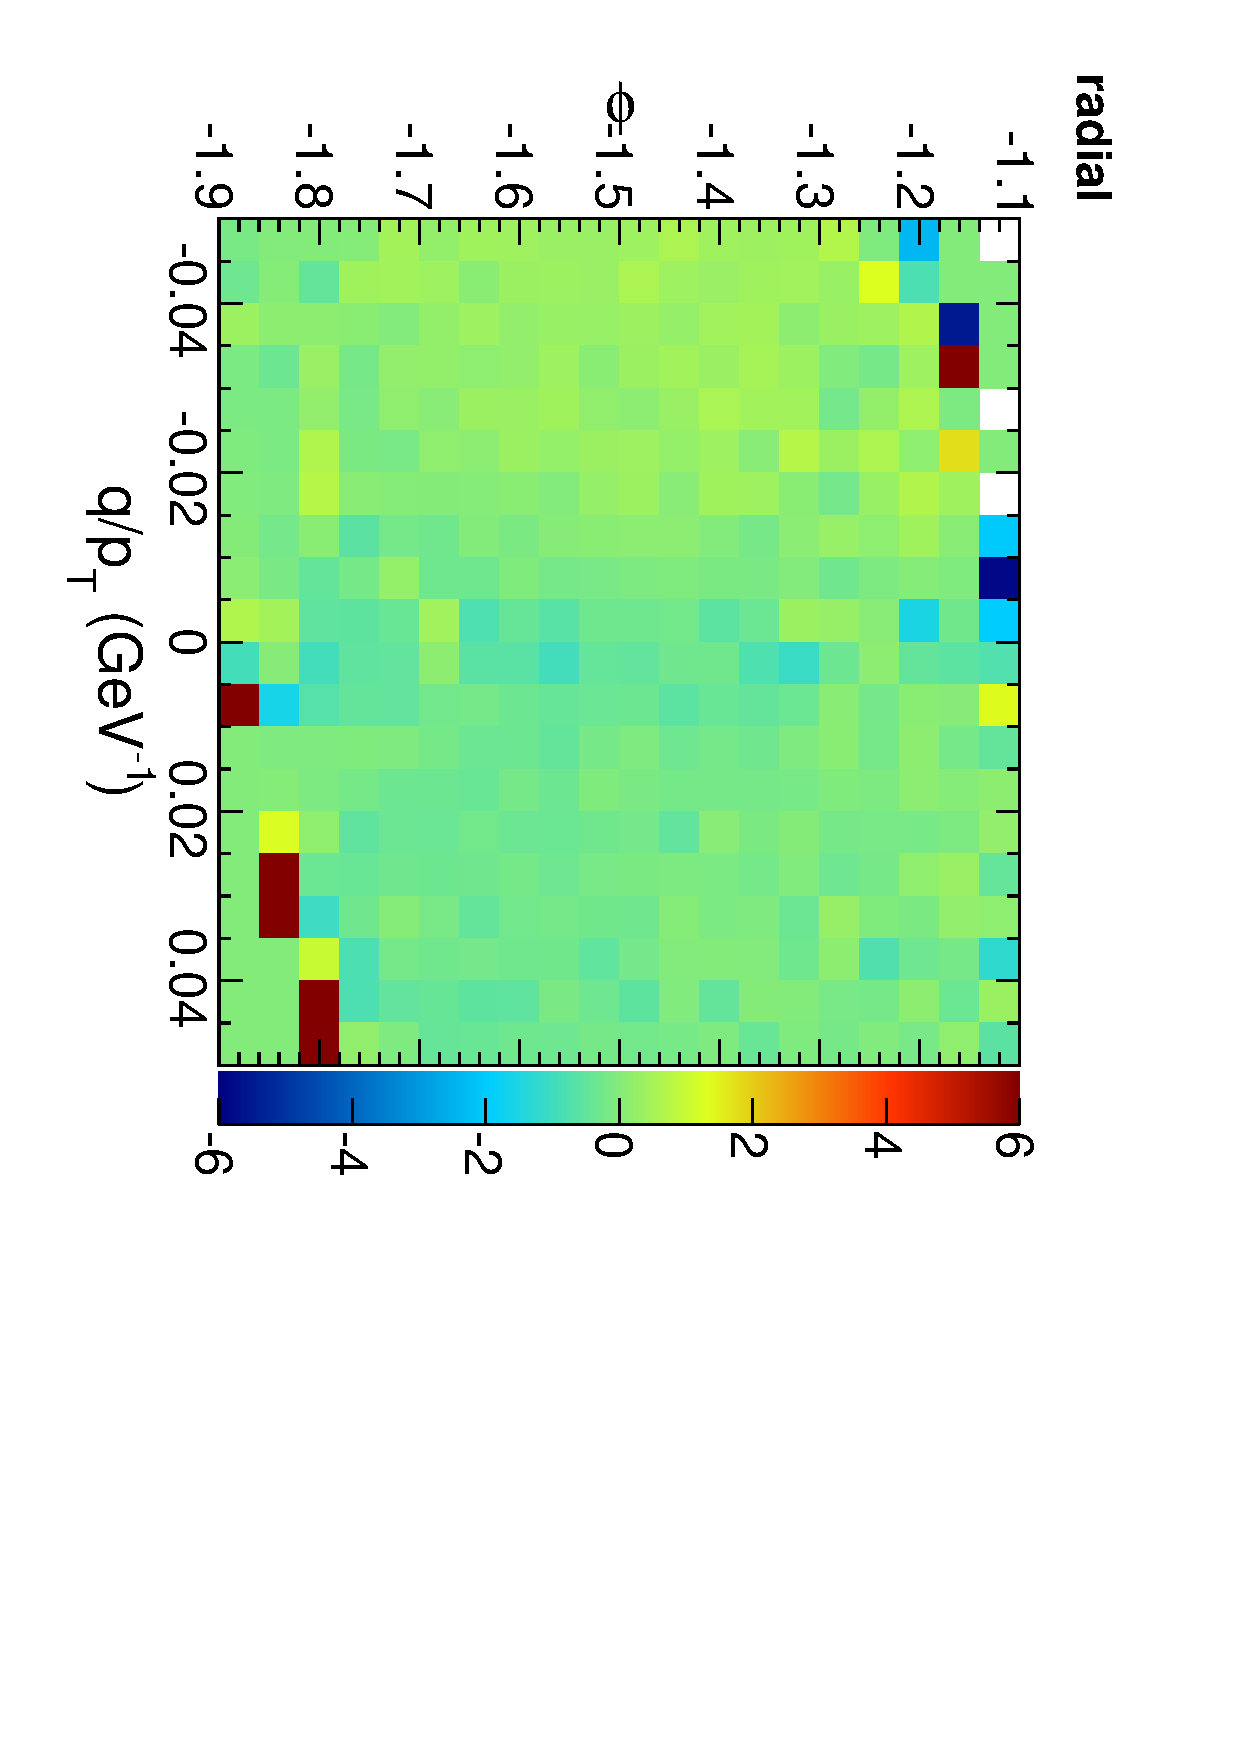
\includegraphics[height=0.32\linewidth, angle=90]{residx-phi-qoverpt_radial.pdf}
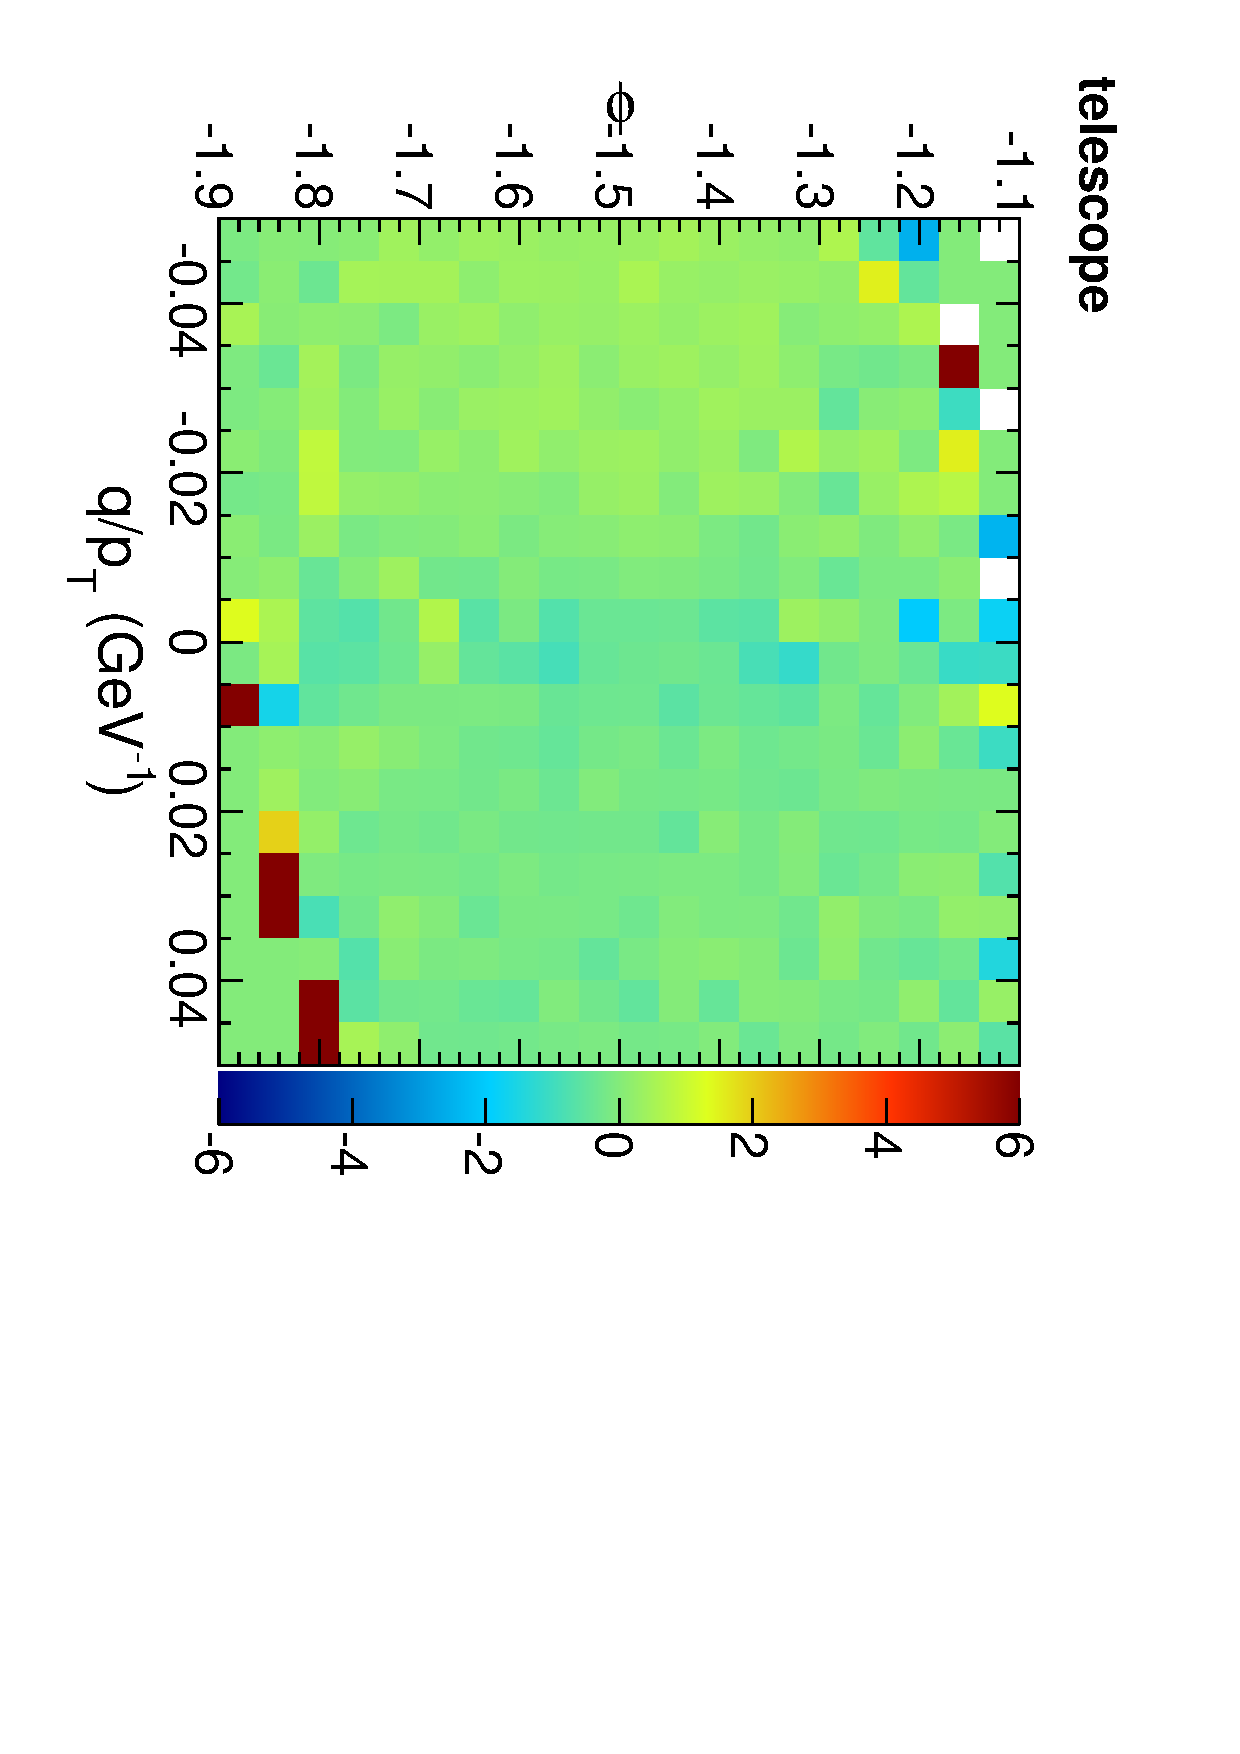
\includegraphics[height=0.32\linewidth, angle=90]{residx-phi-qoverpt_telescope.pdf}
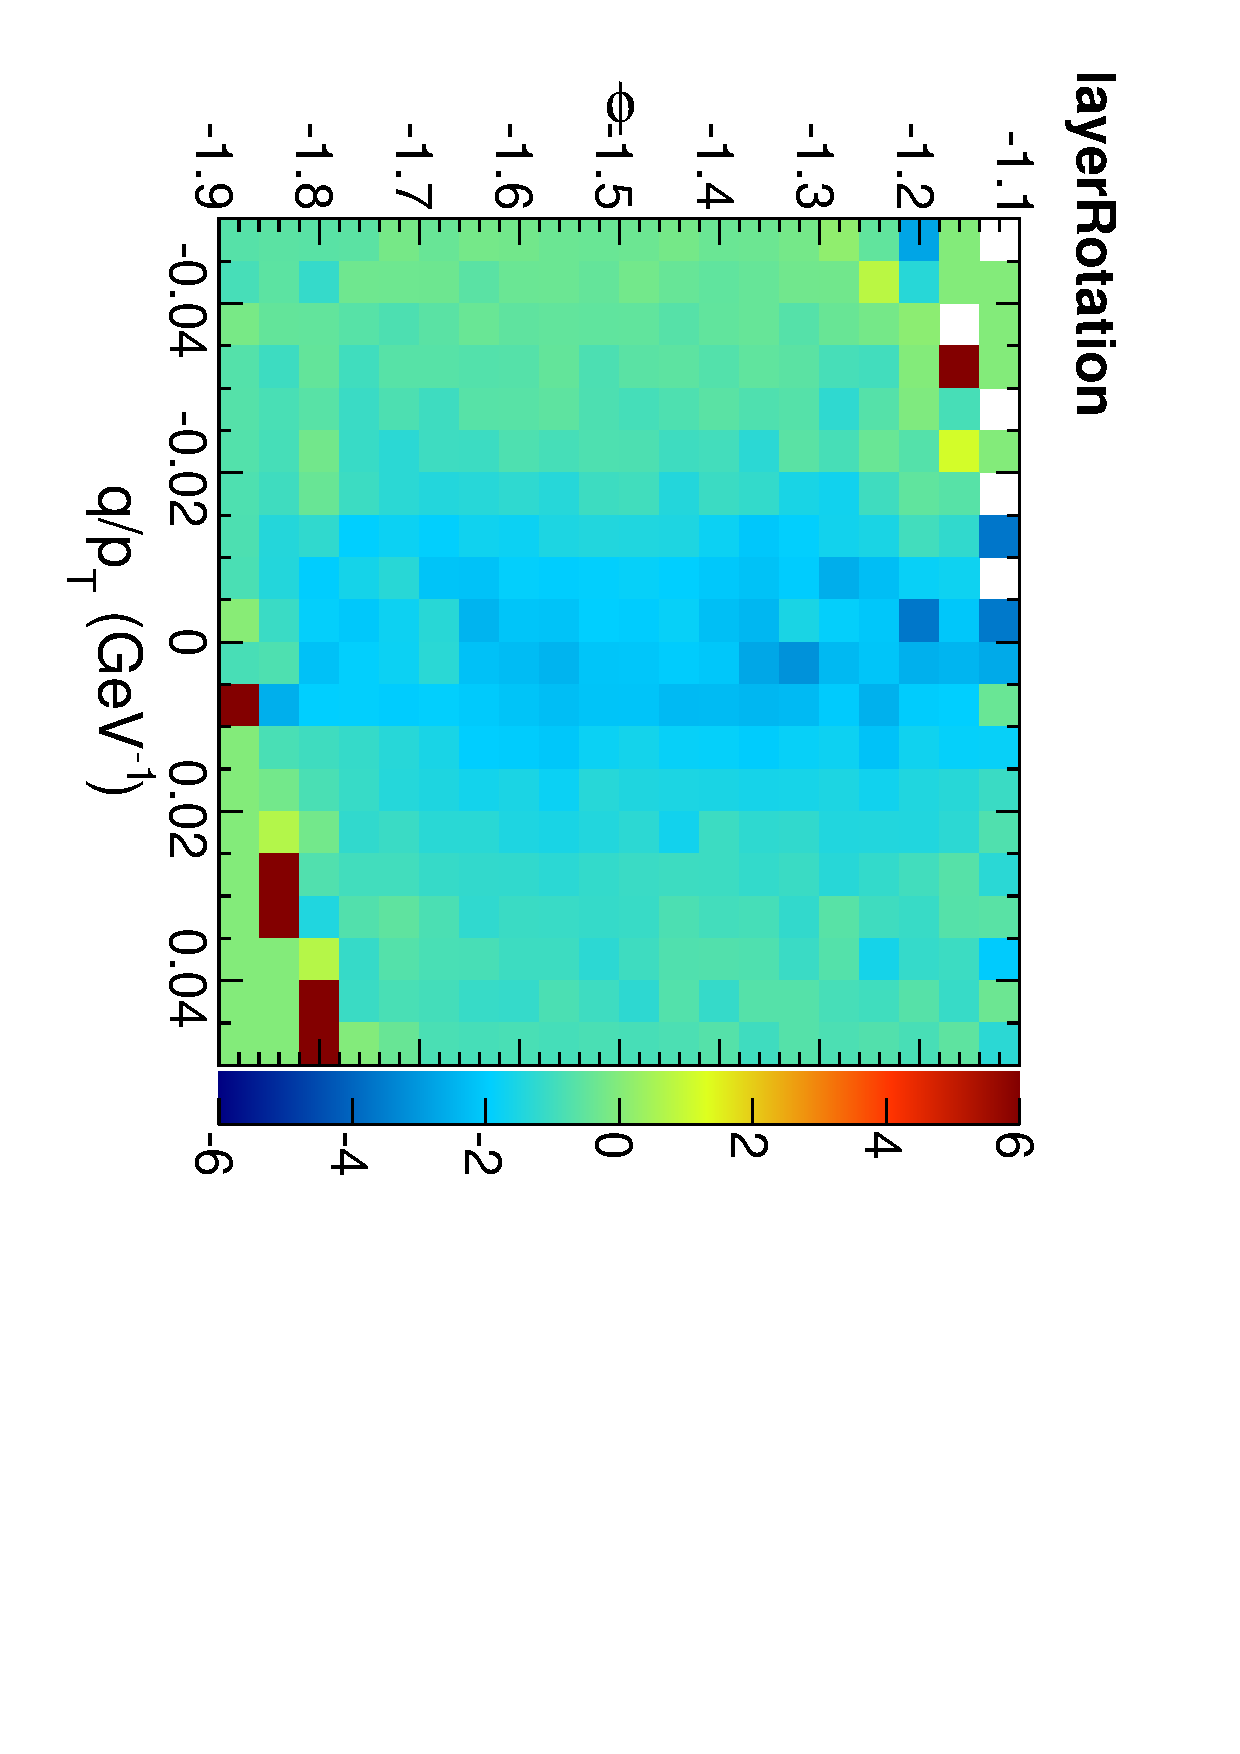
\includegraphics[height=0.32\linewidth, angle=90]{residx-phi-qoverpt_layerRotation.pdf}

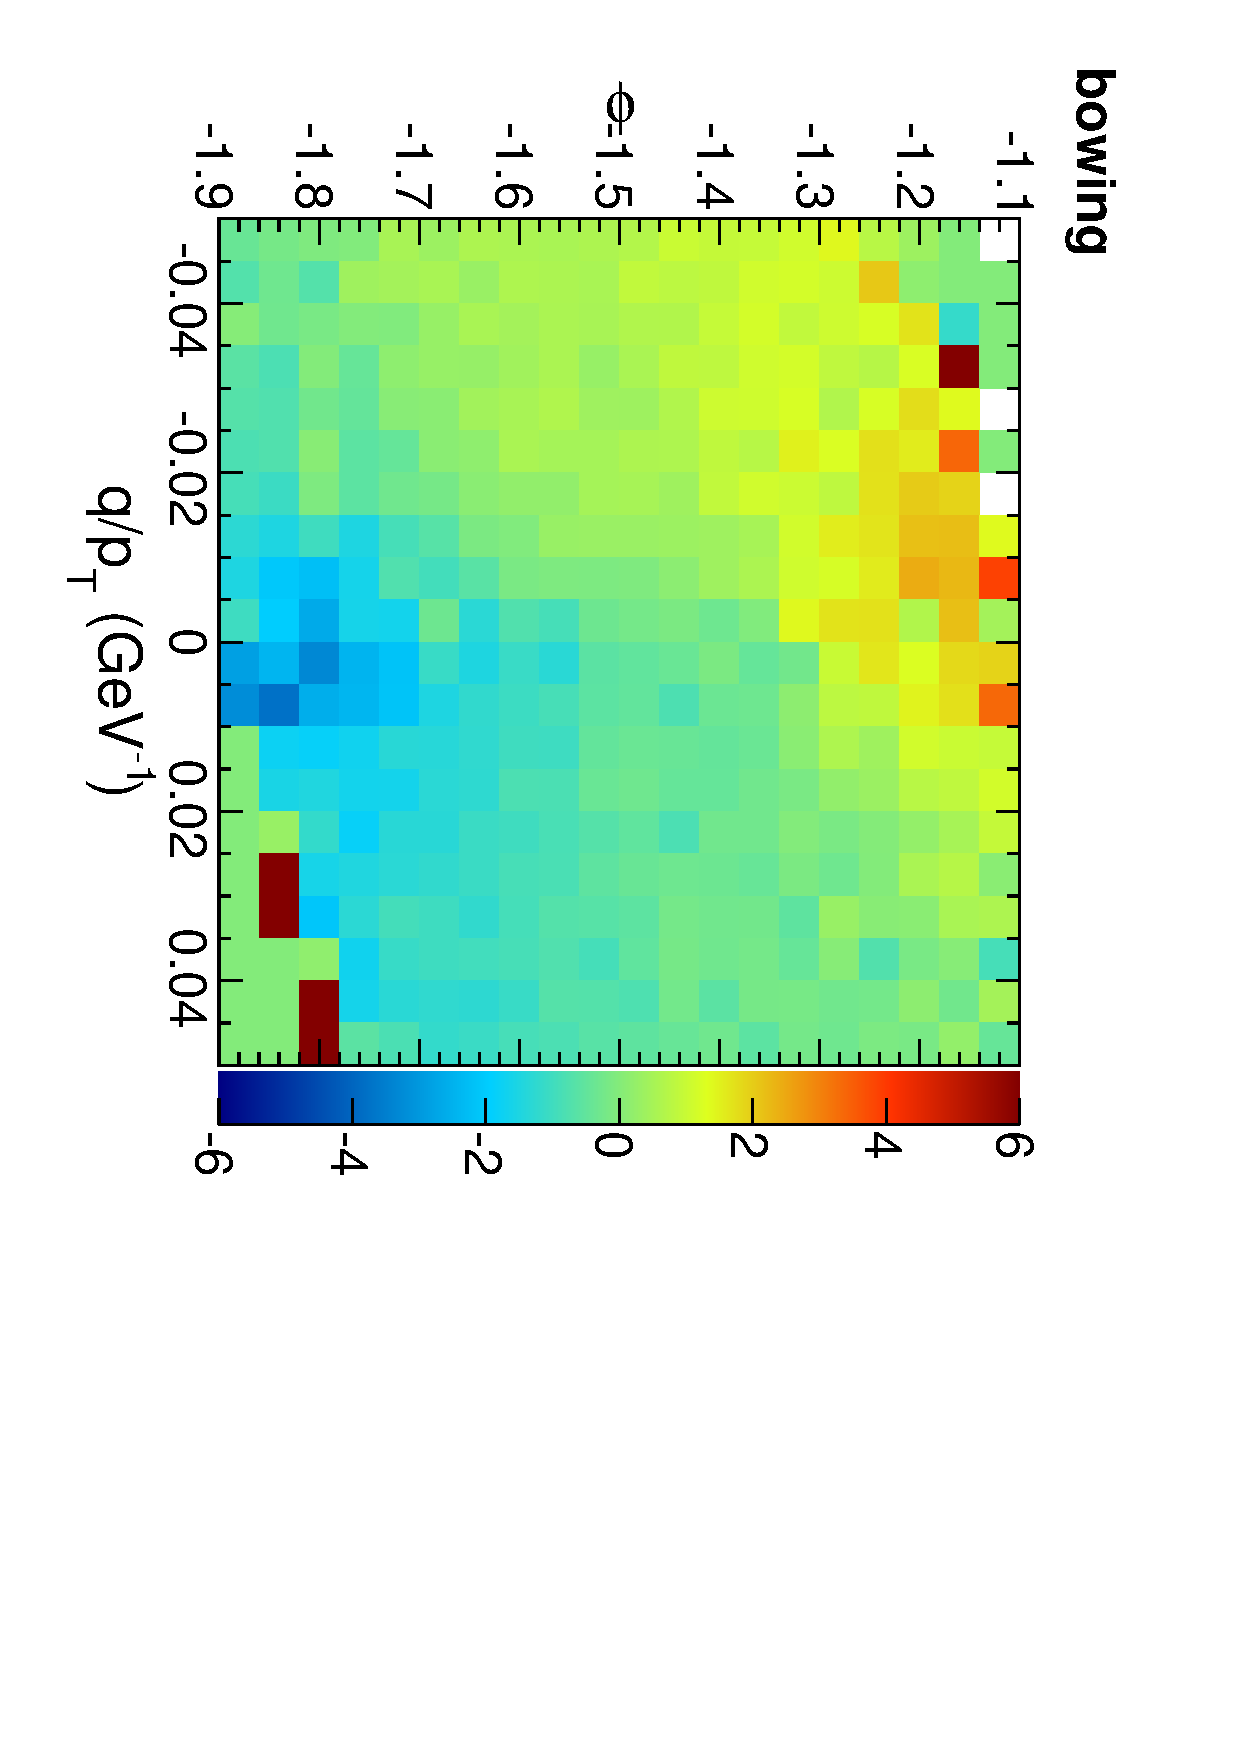
\includegraphics[height=0.32\linewidth, angle=90]{residx-phi-qoverpt_bowing.pdf}
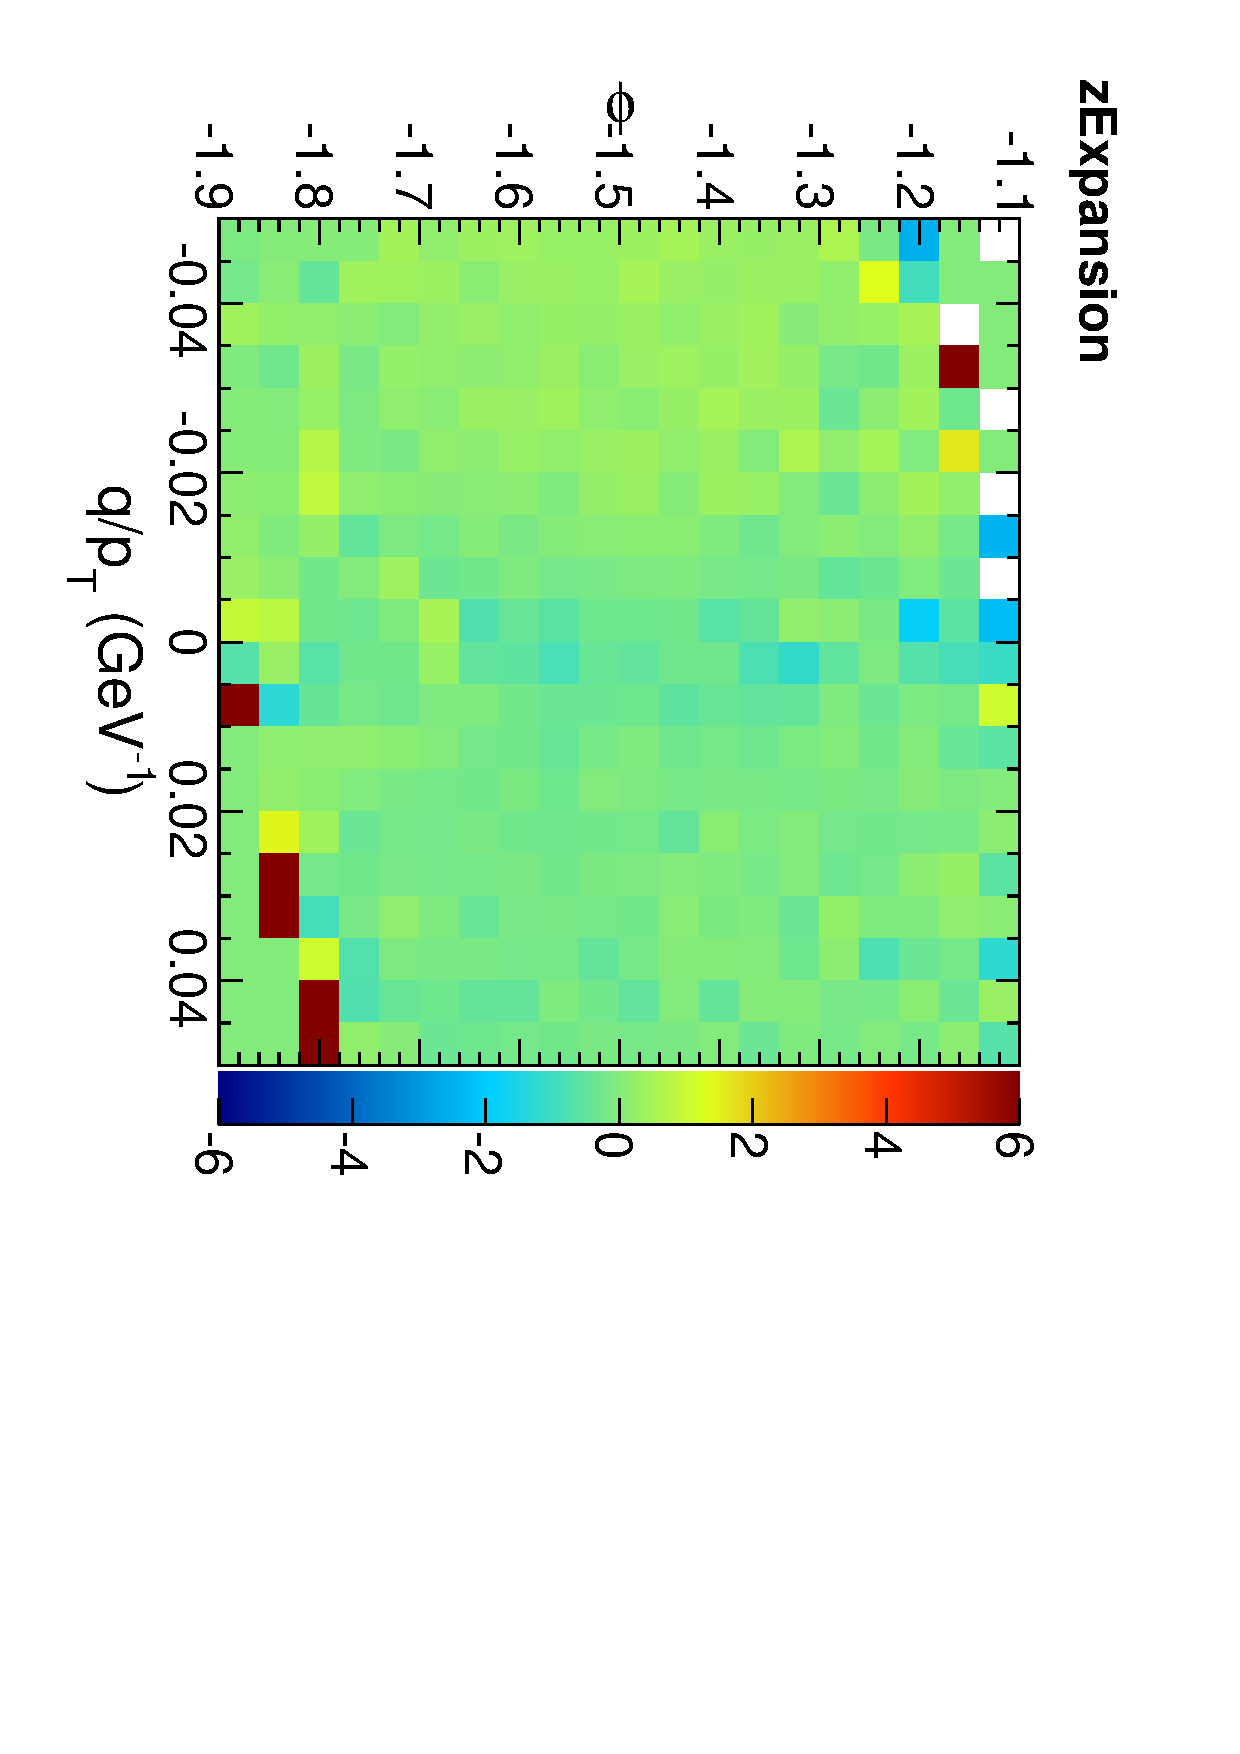
\includegraphics[height=0.32\linewidth, angle=90]{residx-phi-qoverpt_zExpansion.pdf}
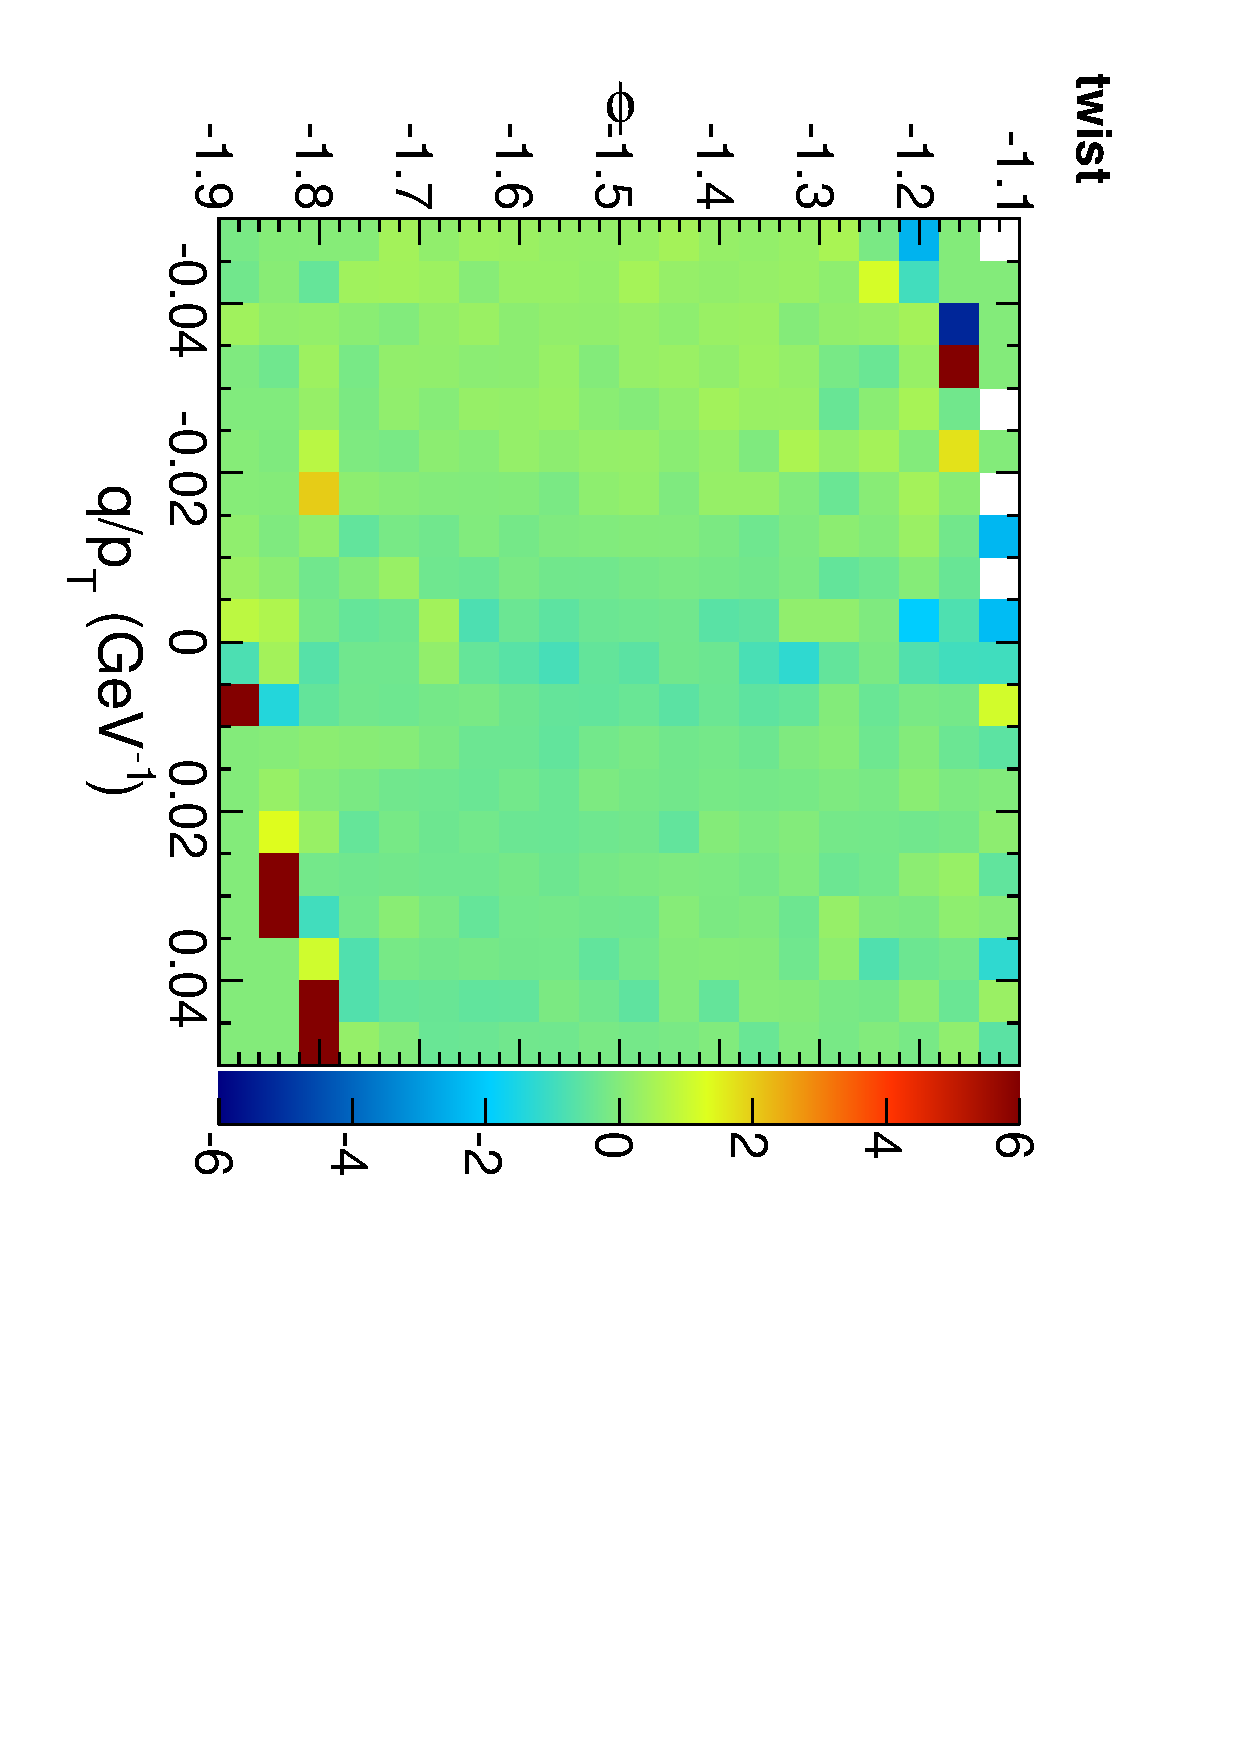
\includegraphics[height=0.32\linewidth, angle=90]{residx-phi-qoverpt_twist.pdf}

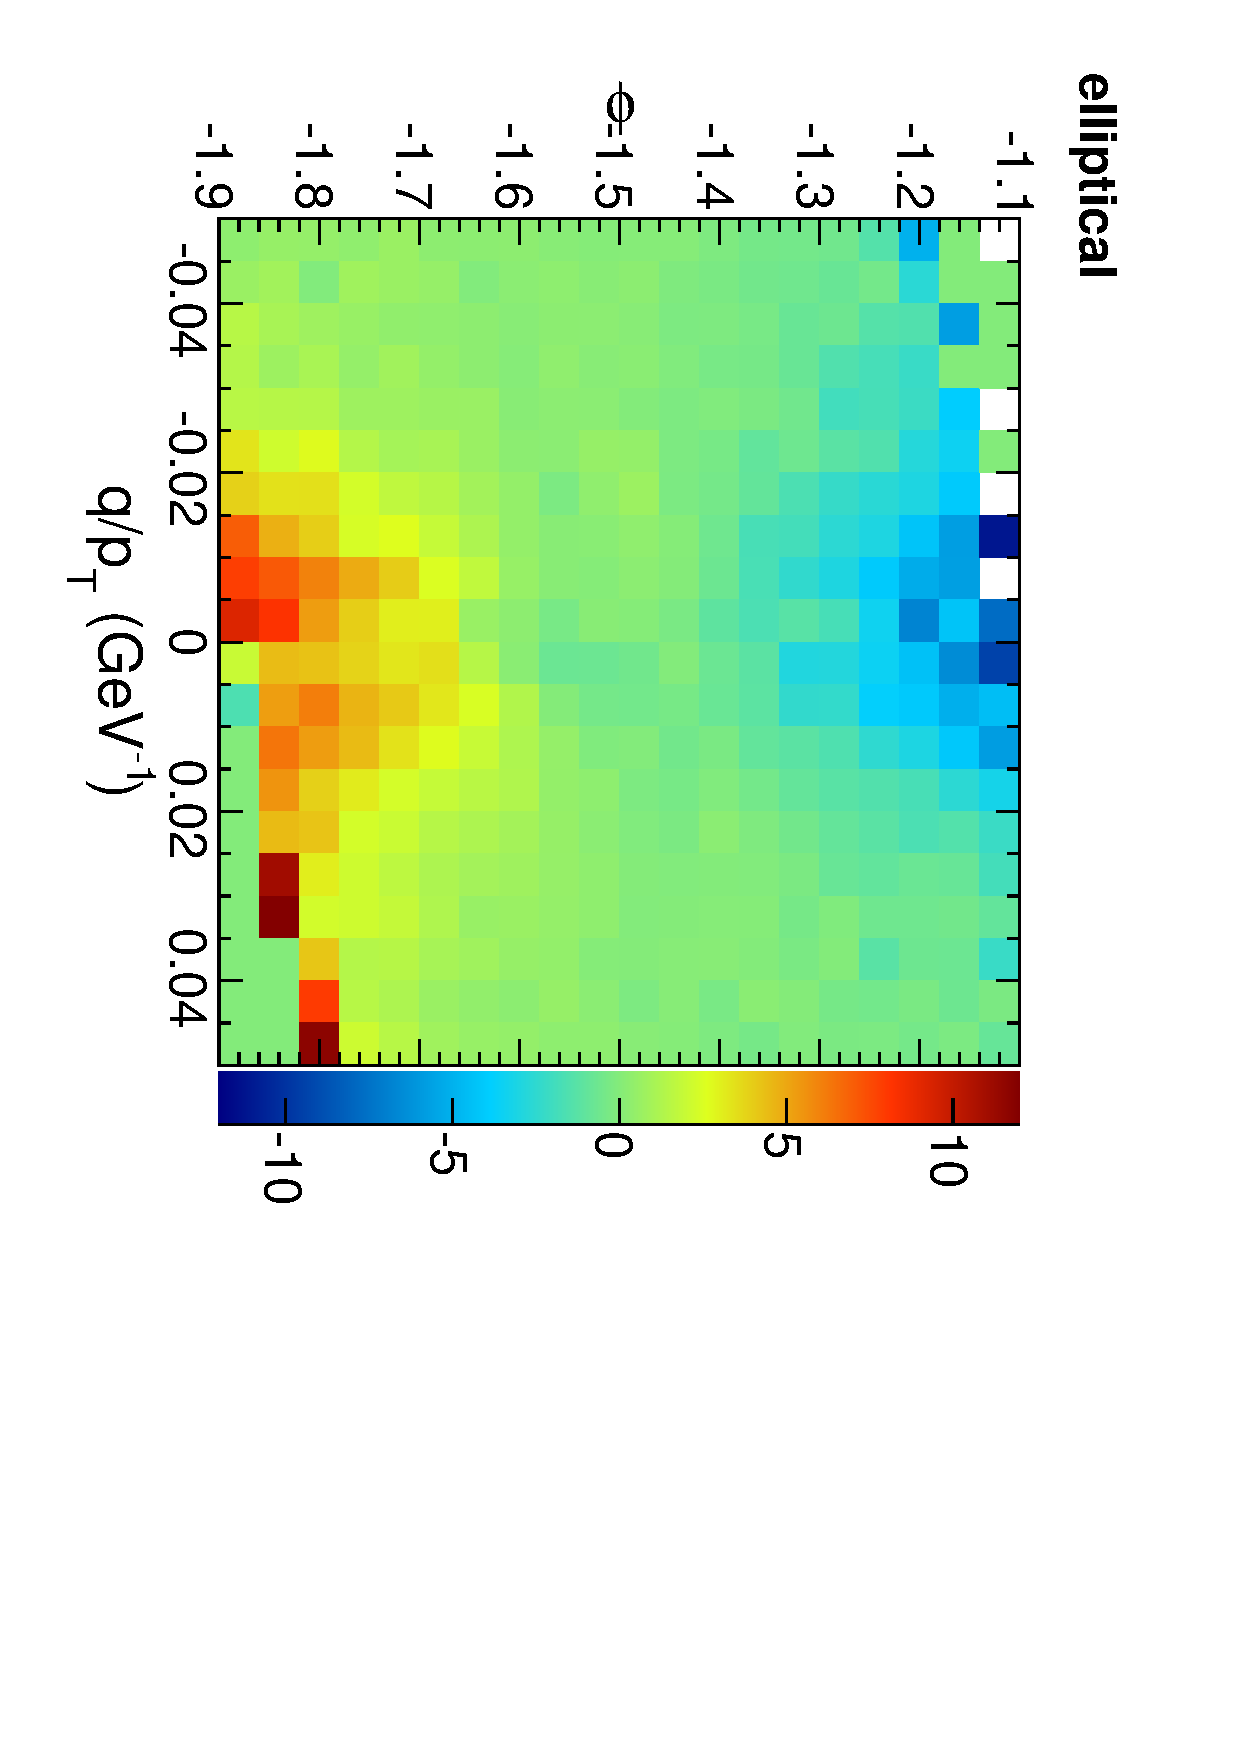
\includegraphics[height=0.32\linewidth, angle=90]{residx-phi-qoverpt_elliptical.pdf}
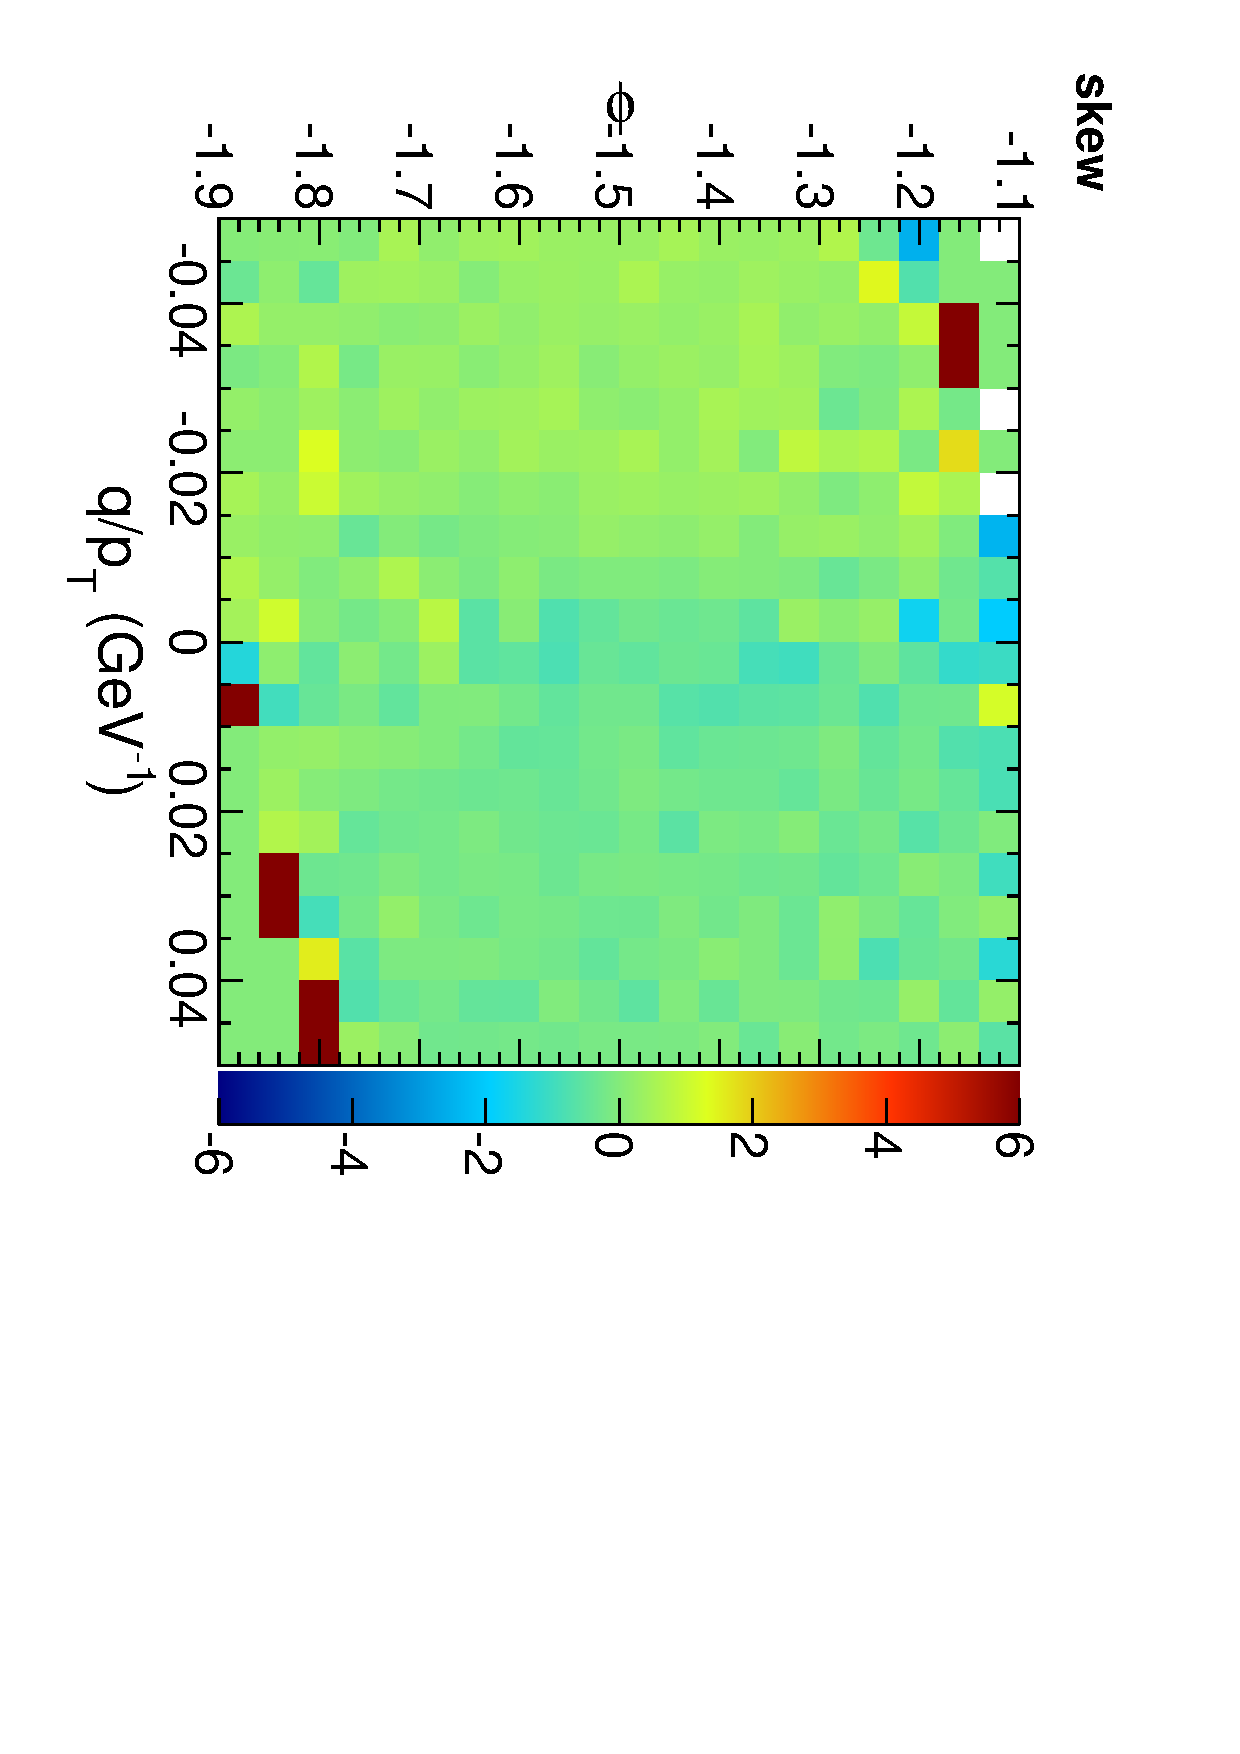
\includegraphics[height=0.32\linewidth, angle=90]{residx-phi-qoverpt_skew.pdf}
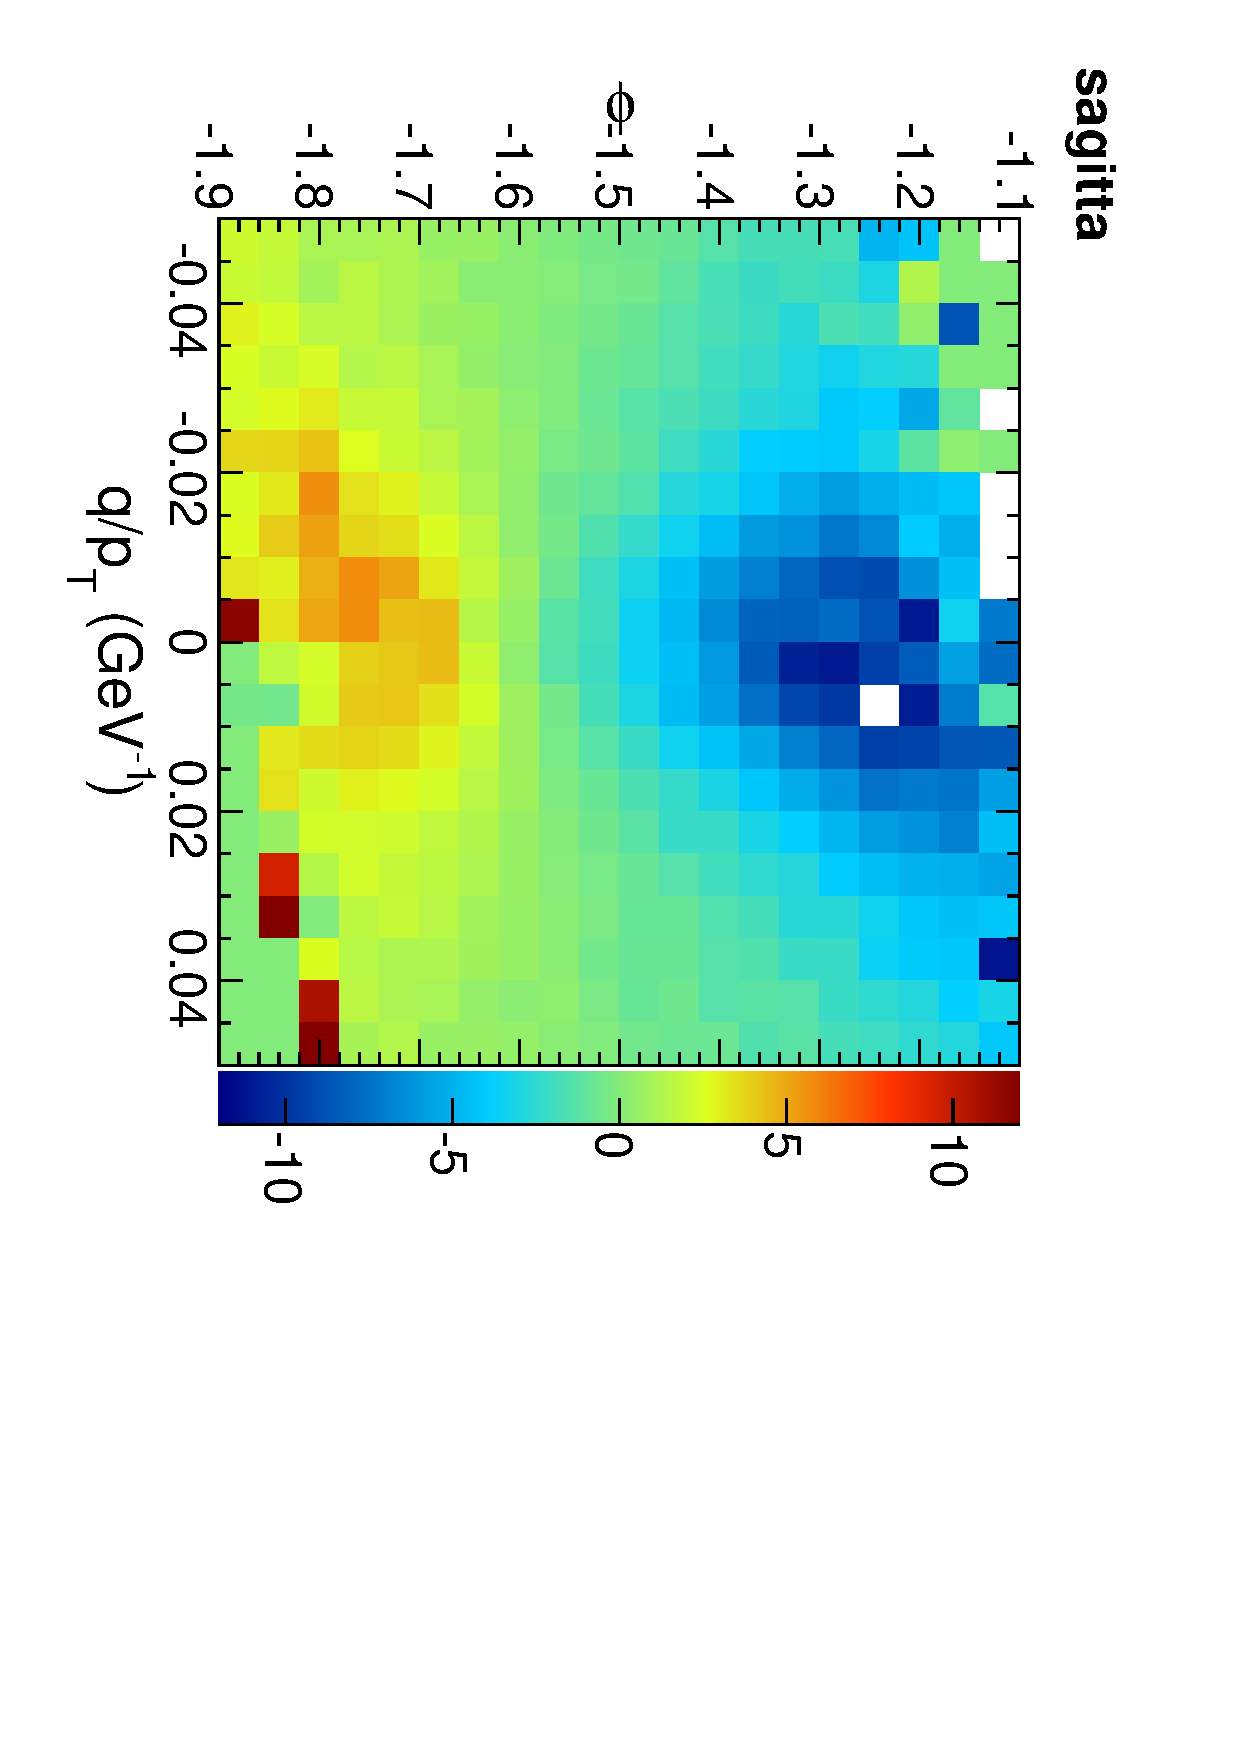
\includegraphics[height=0.32\linewidth, angle=90]{residx-phi-qoverpt_sagitta.pdf}
\end{columns}
\end{frame}

\begin{frame}
\frametitle{Residual vs.~$d_{xy}$ and $\phi$ (high $p_T$)}

\begin{itemize}
\item ``High $p_T$'' means $p_T > 100$~GeV
\item Looks similar to sagitta in this projection, but from the previous two pages, we know that the real distribution is not exactly sagitta
\end{itemize}

\begin{columns}
\column{0.4\linewidth}
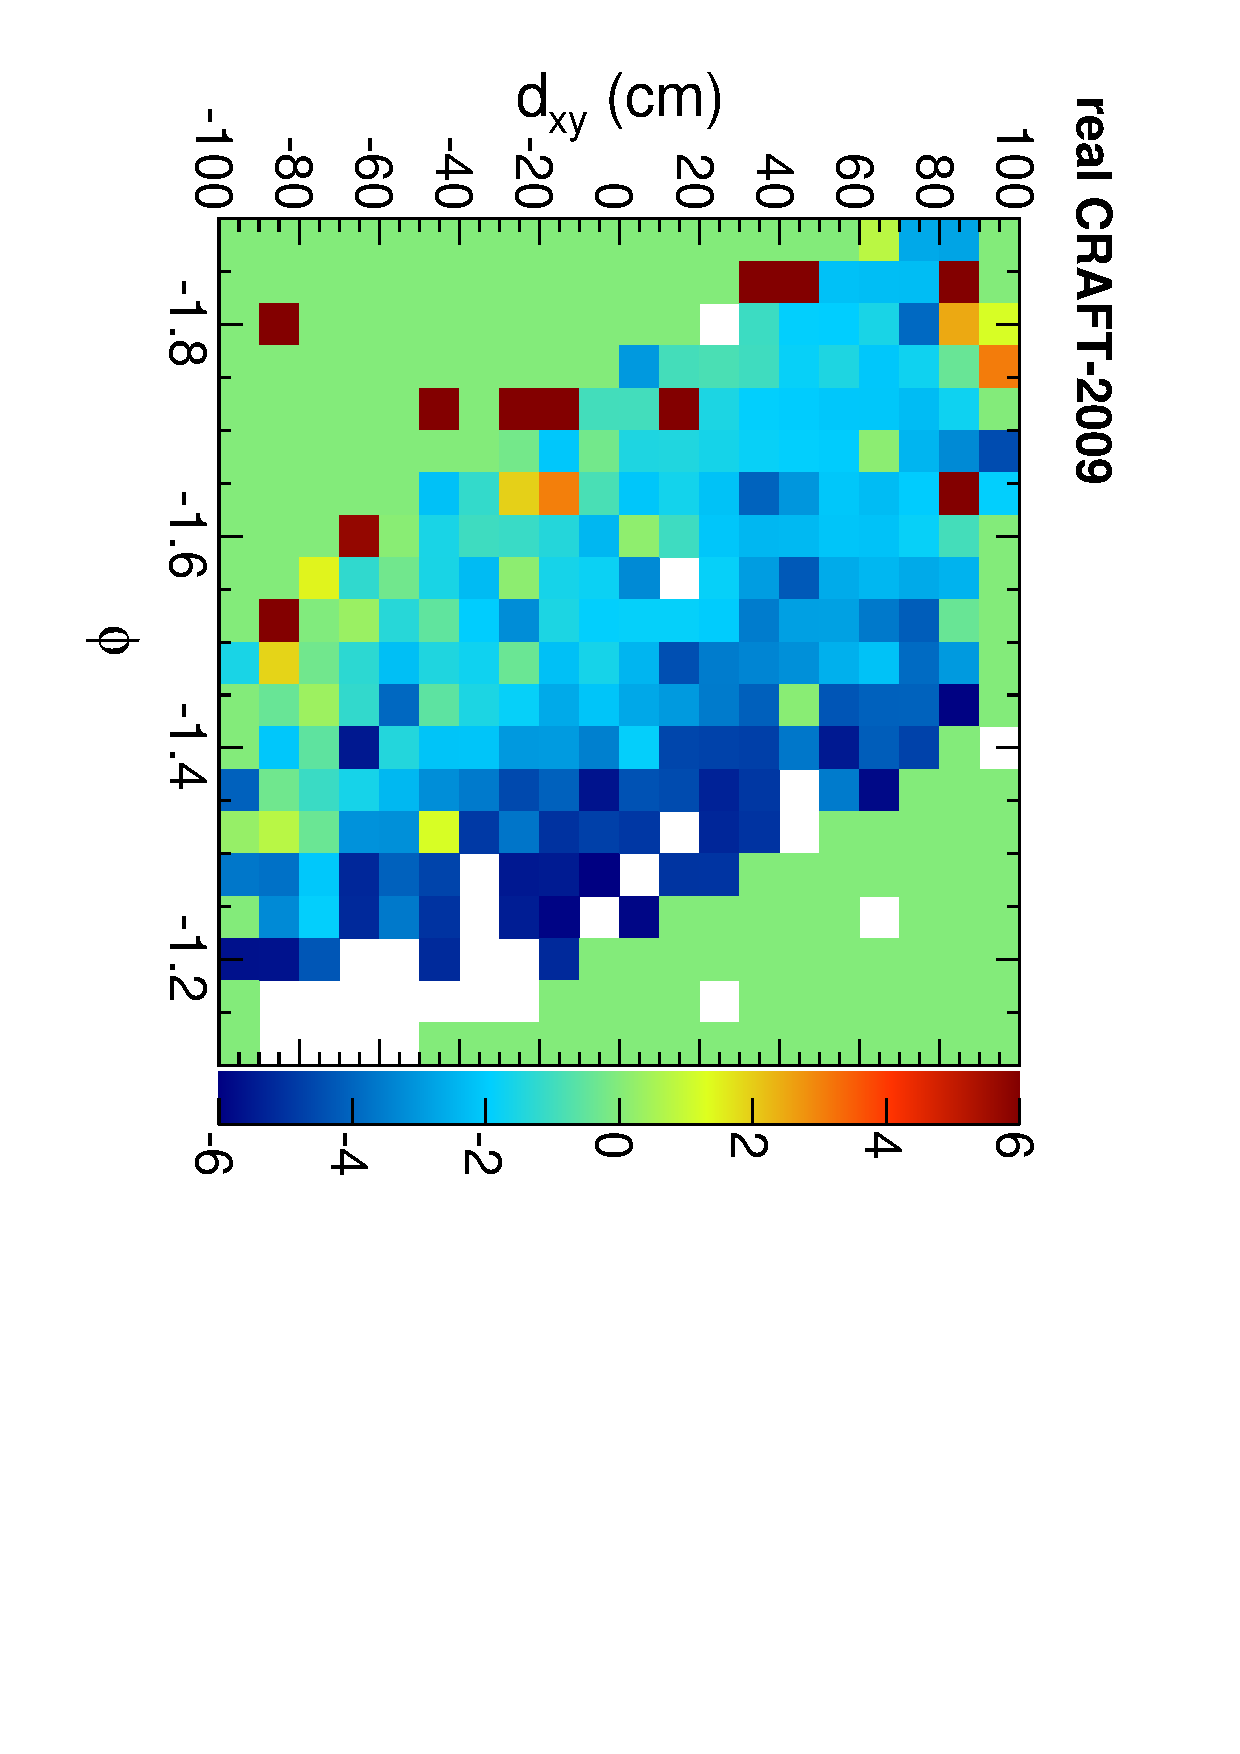
\includegraphics[height=\linewidth, angle=90]{residx-dxy-phi-high_real.pdf}

\column{0.6\linewidth}
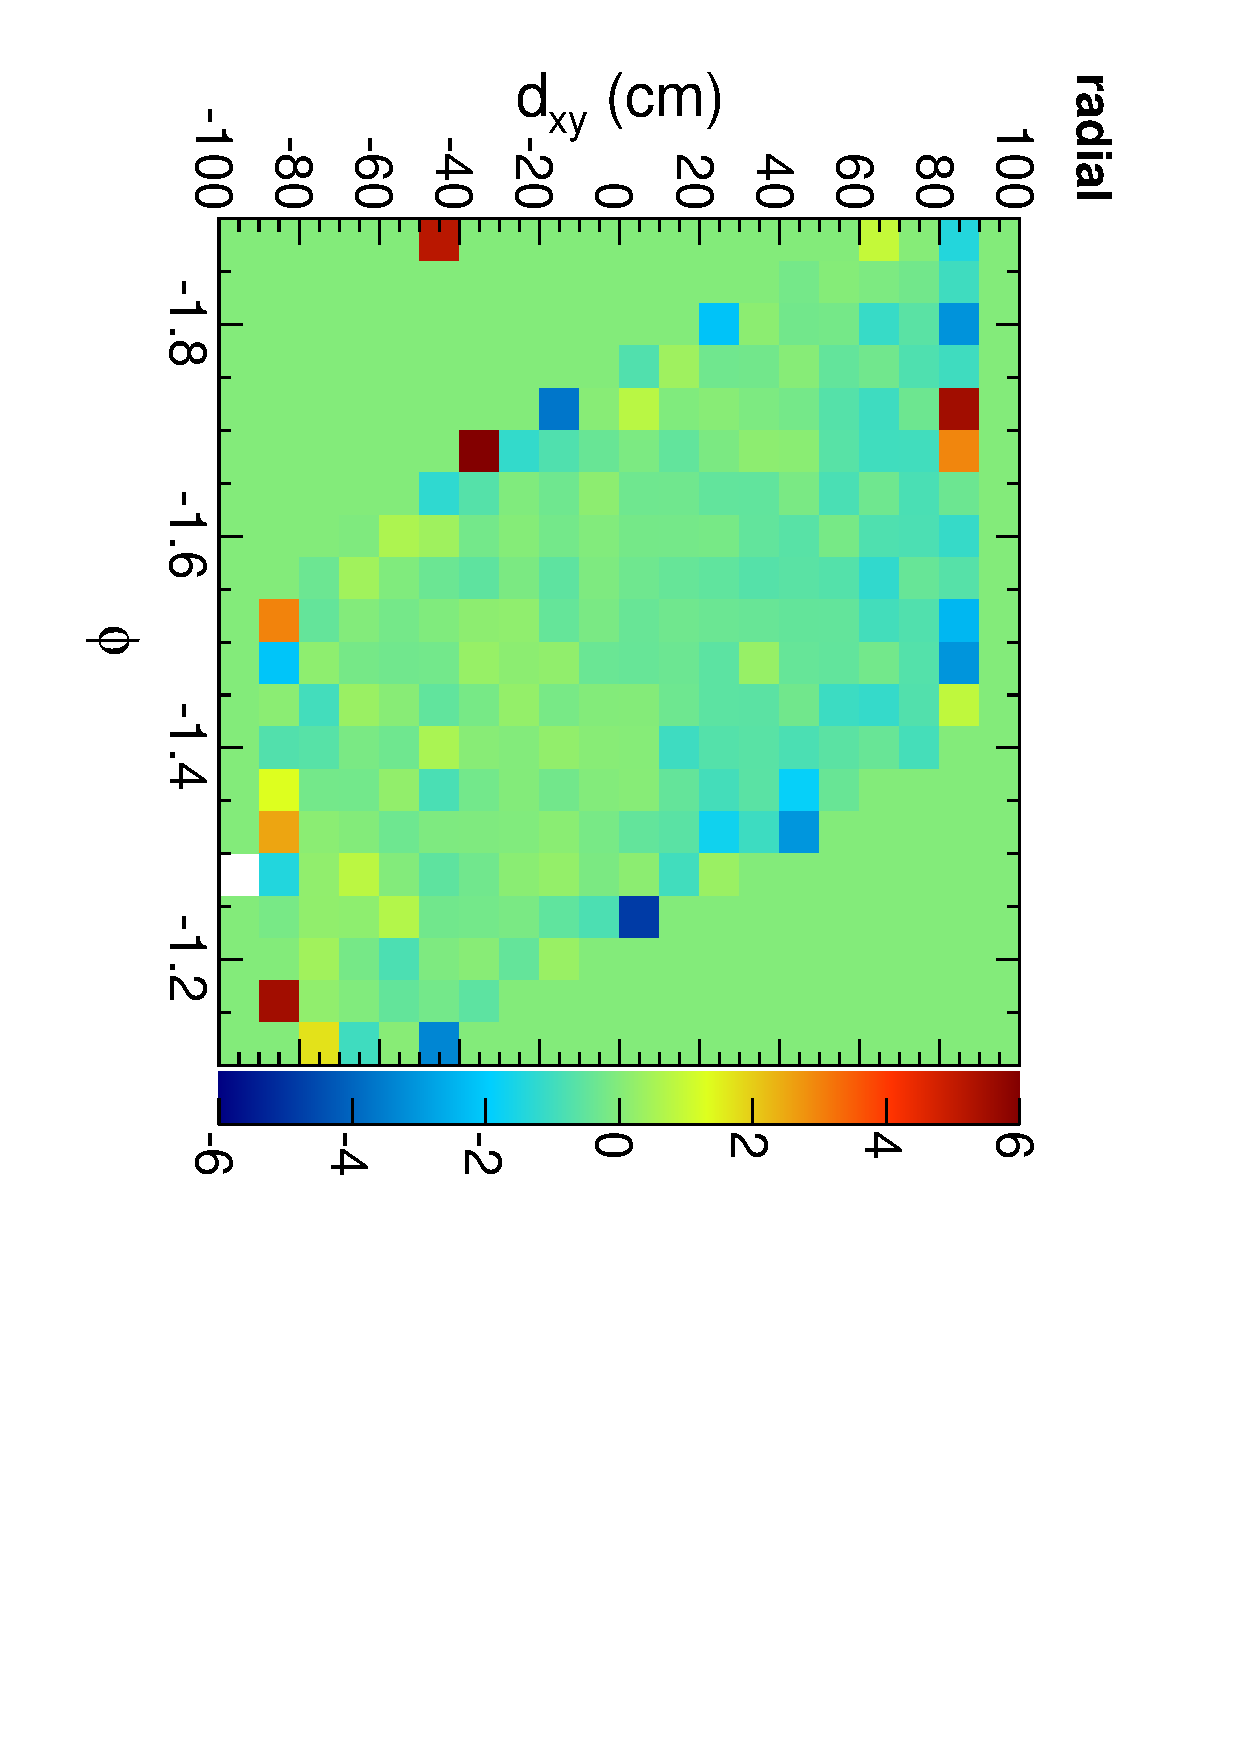
\includegraphics[height=0.32\linewidth, angle=90]{residx-dxy-phi-high_radial.pdf}
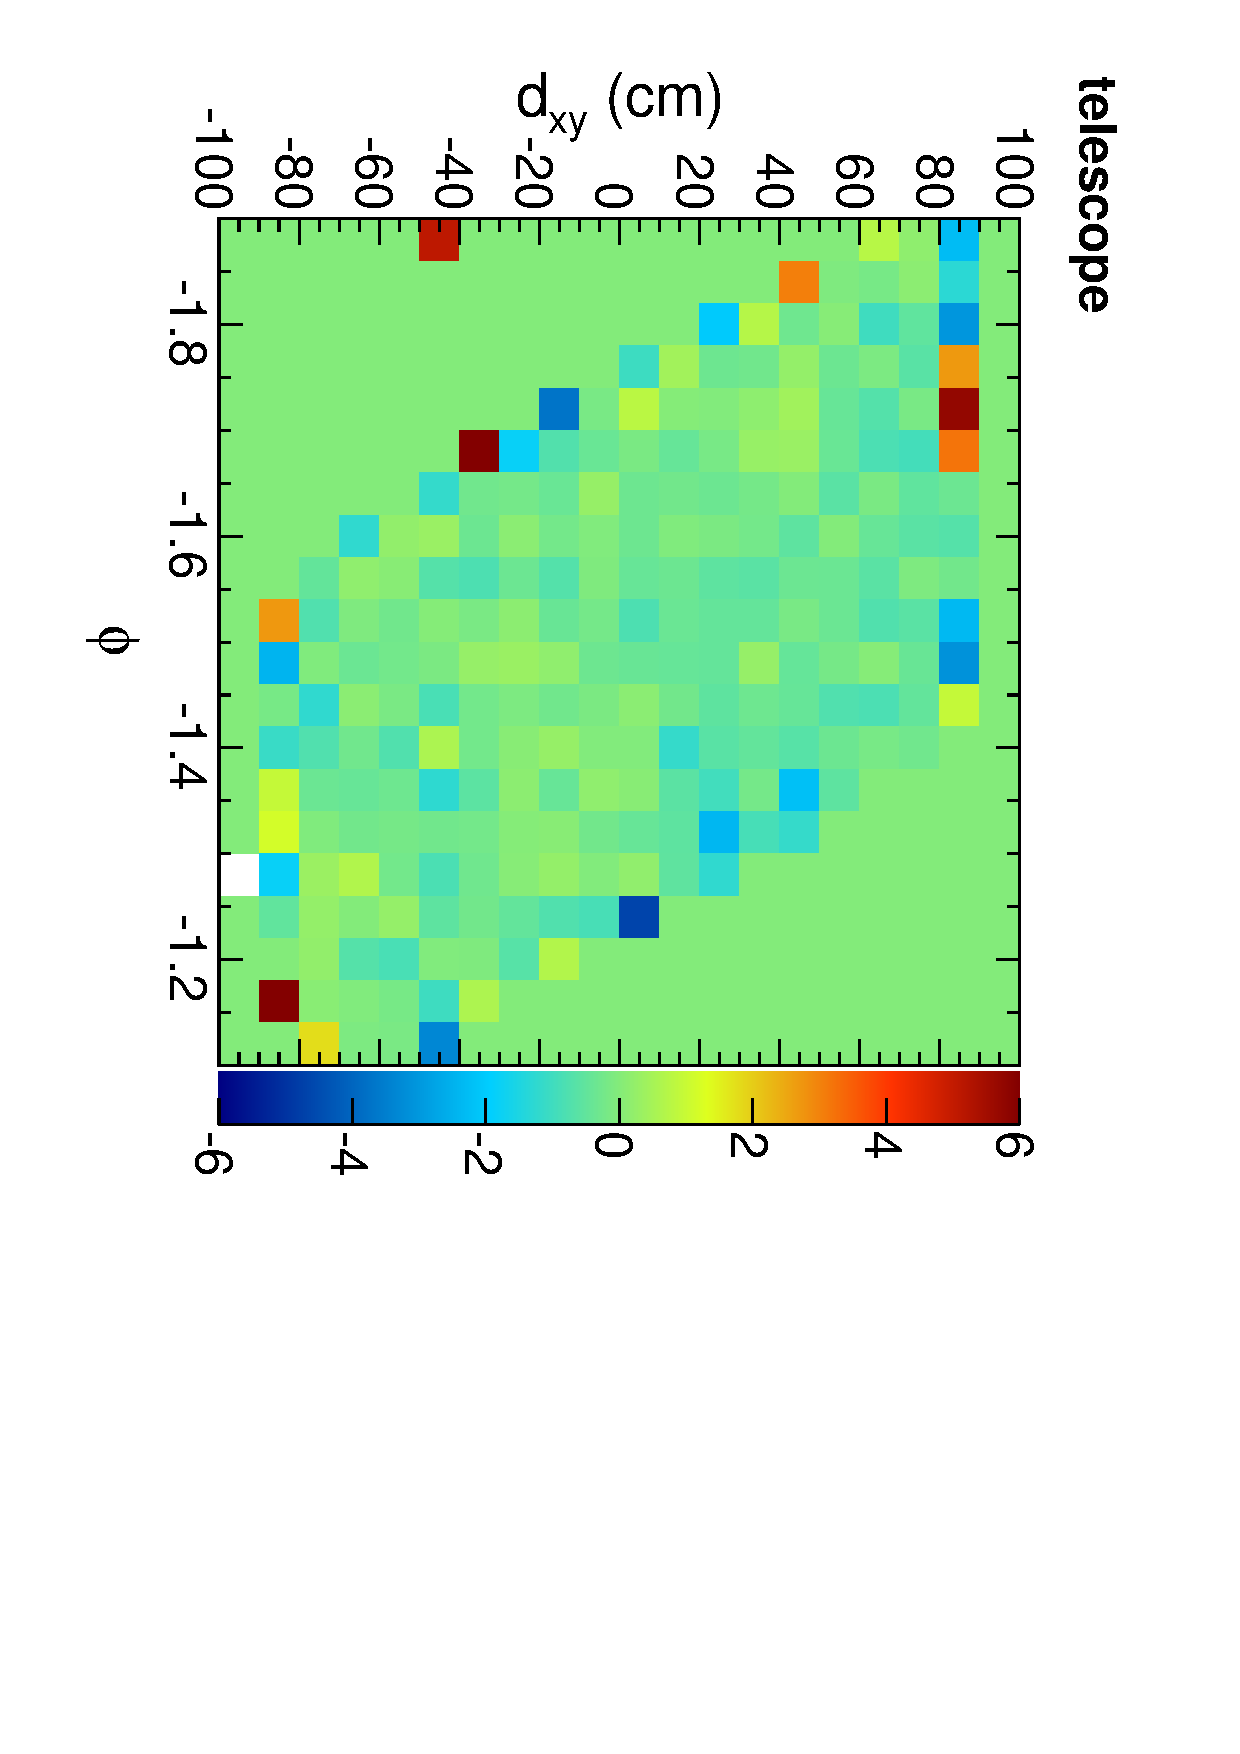
\includegraphics[height=0.32\linewidth, angle=90]{residx-dxy-phi-high_telescope.pdf}
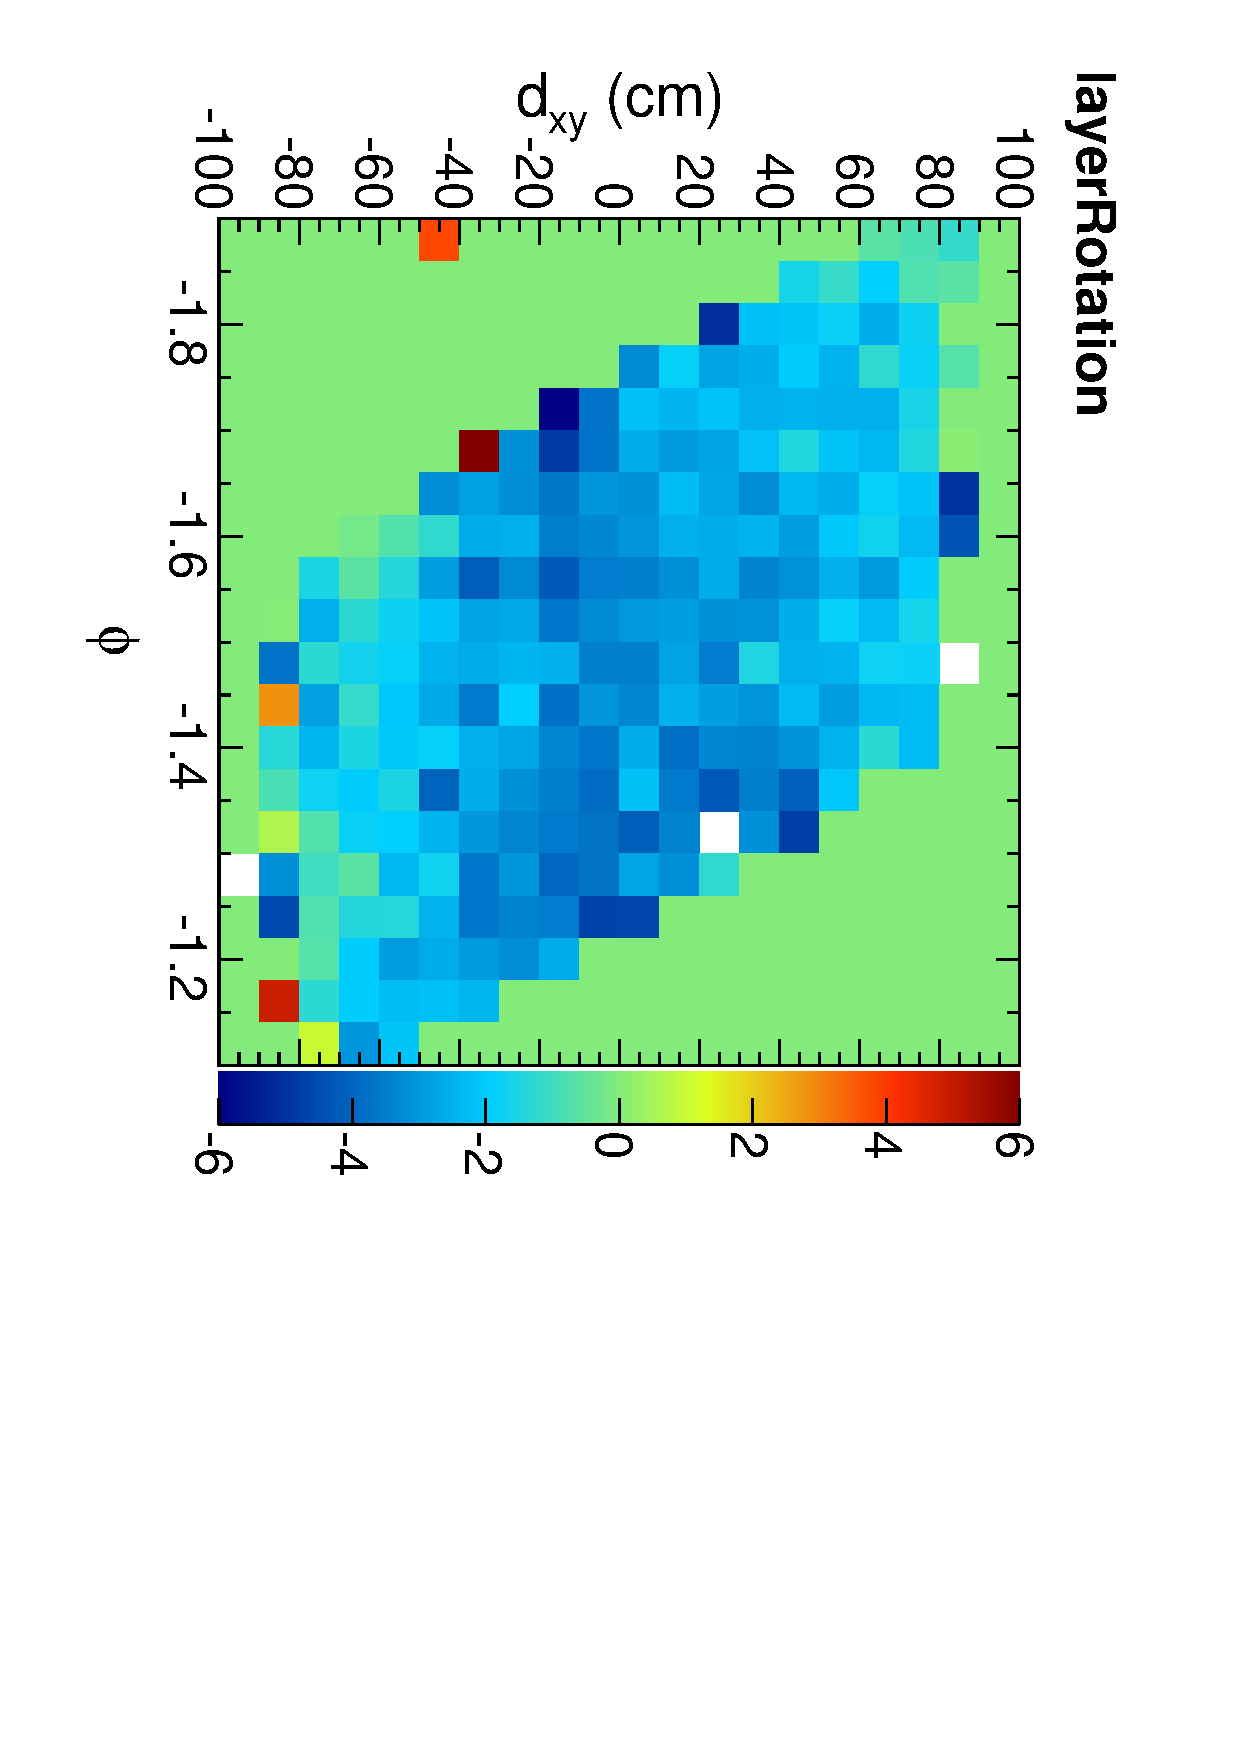
\includegraphics[height=0.32\linewidth, angle=90]{residx-dxy-phi-high_layerRotation.pdf}

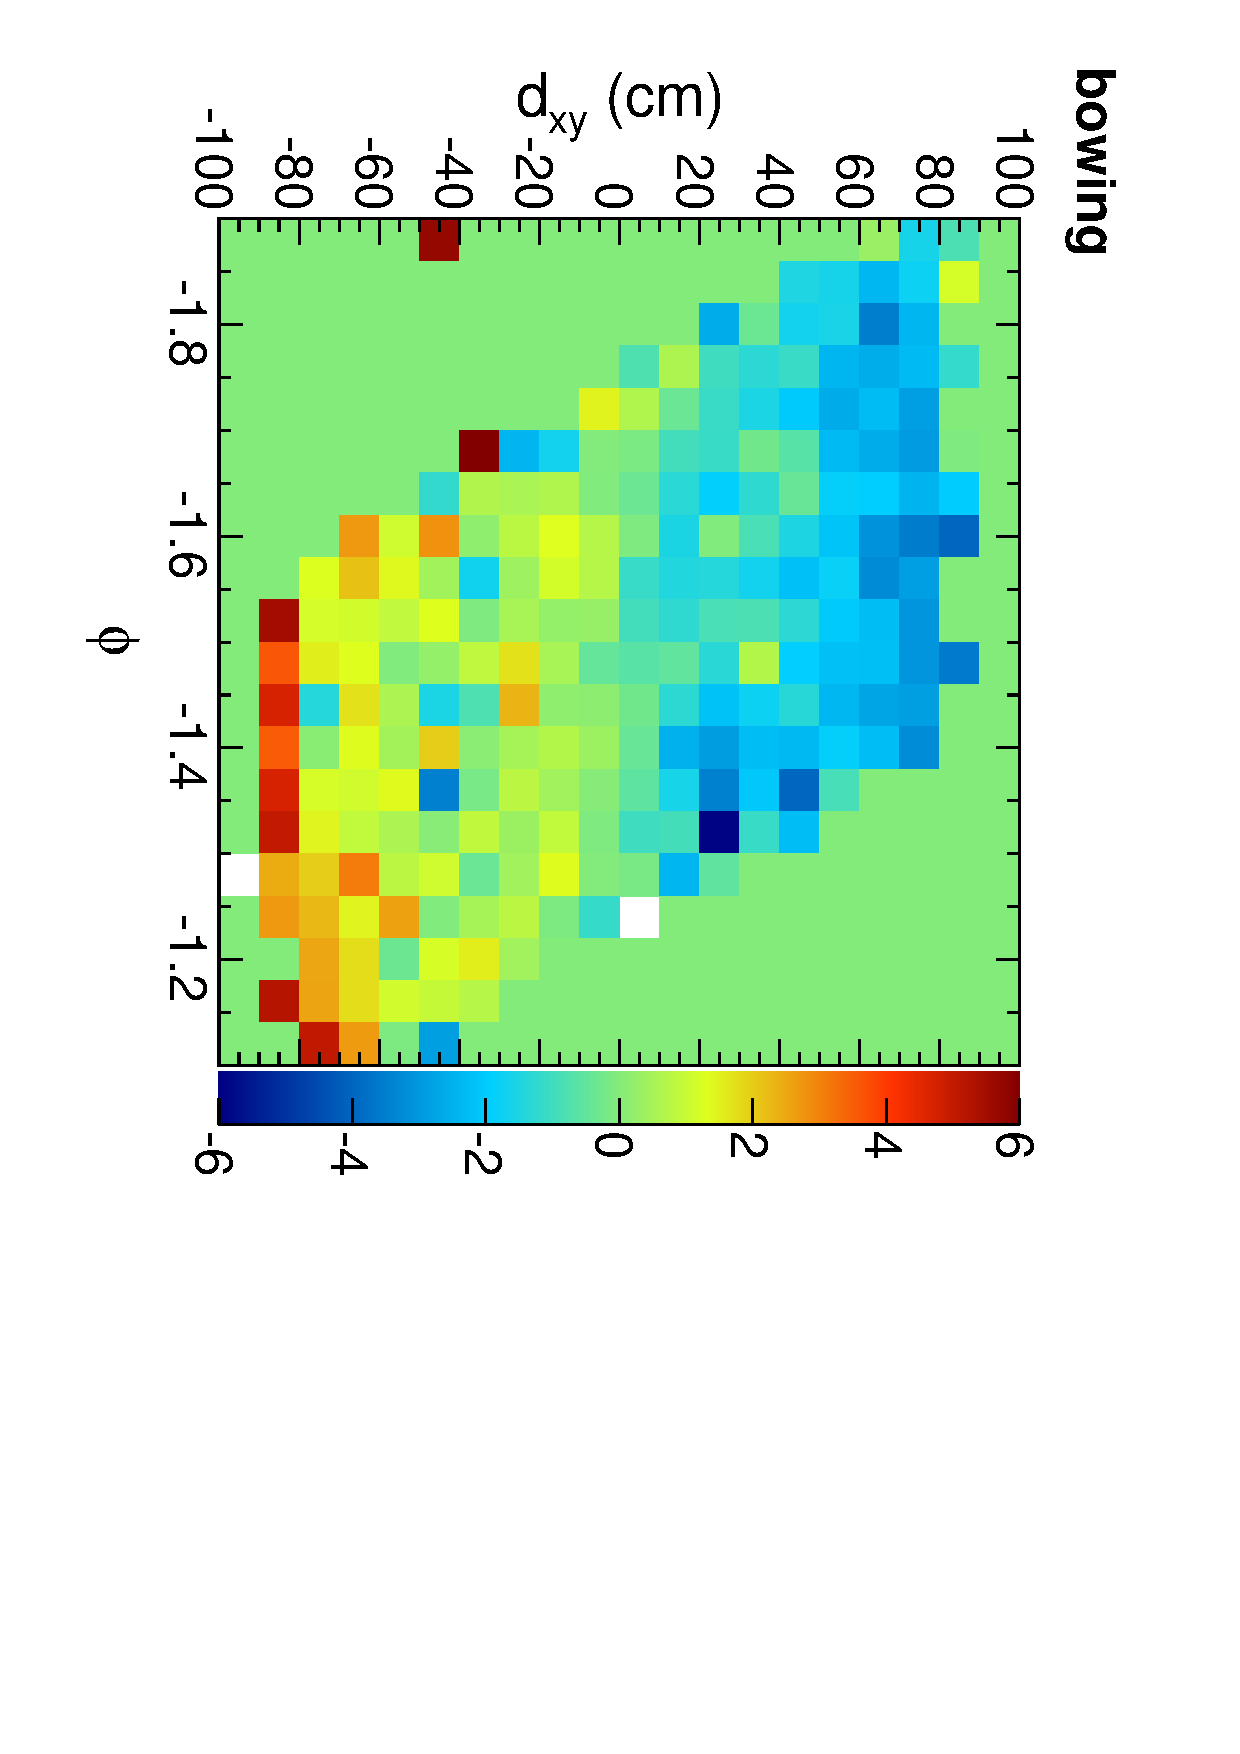
\includegraphics[height=0.32\linewidth, angle=90]{residx-dxy-phi-high_bowing.pdf}
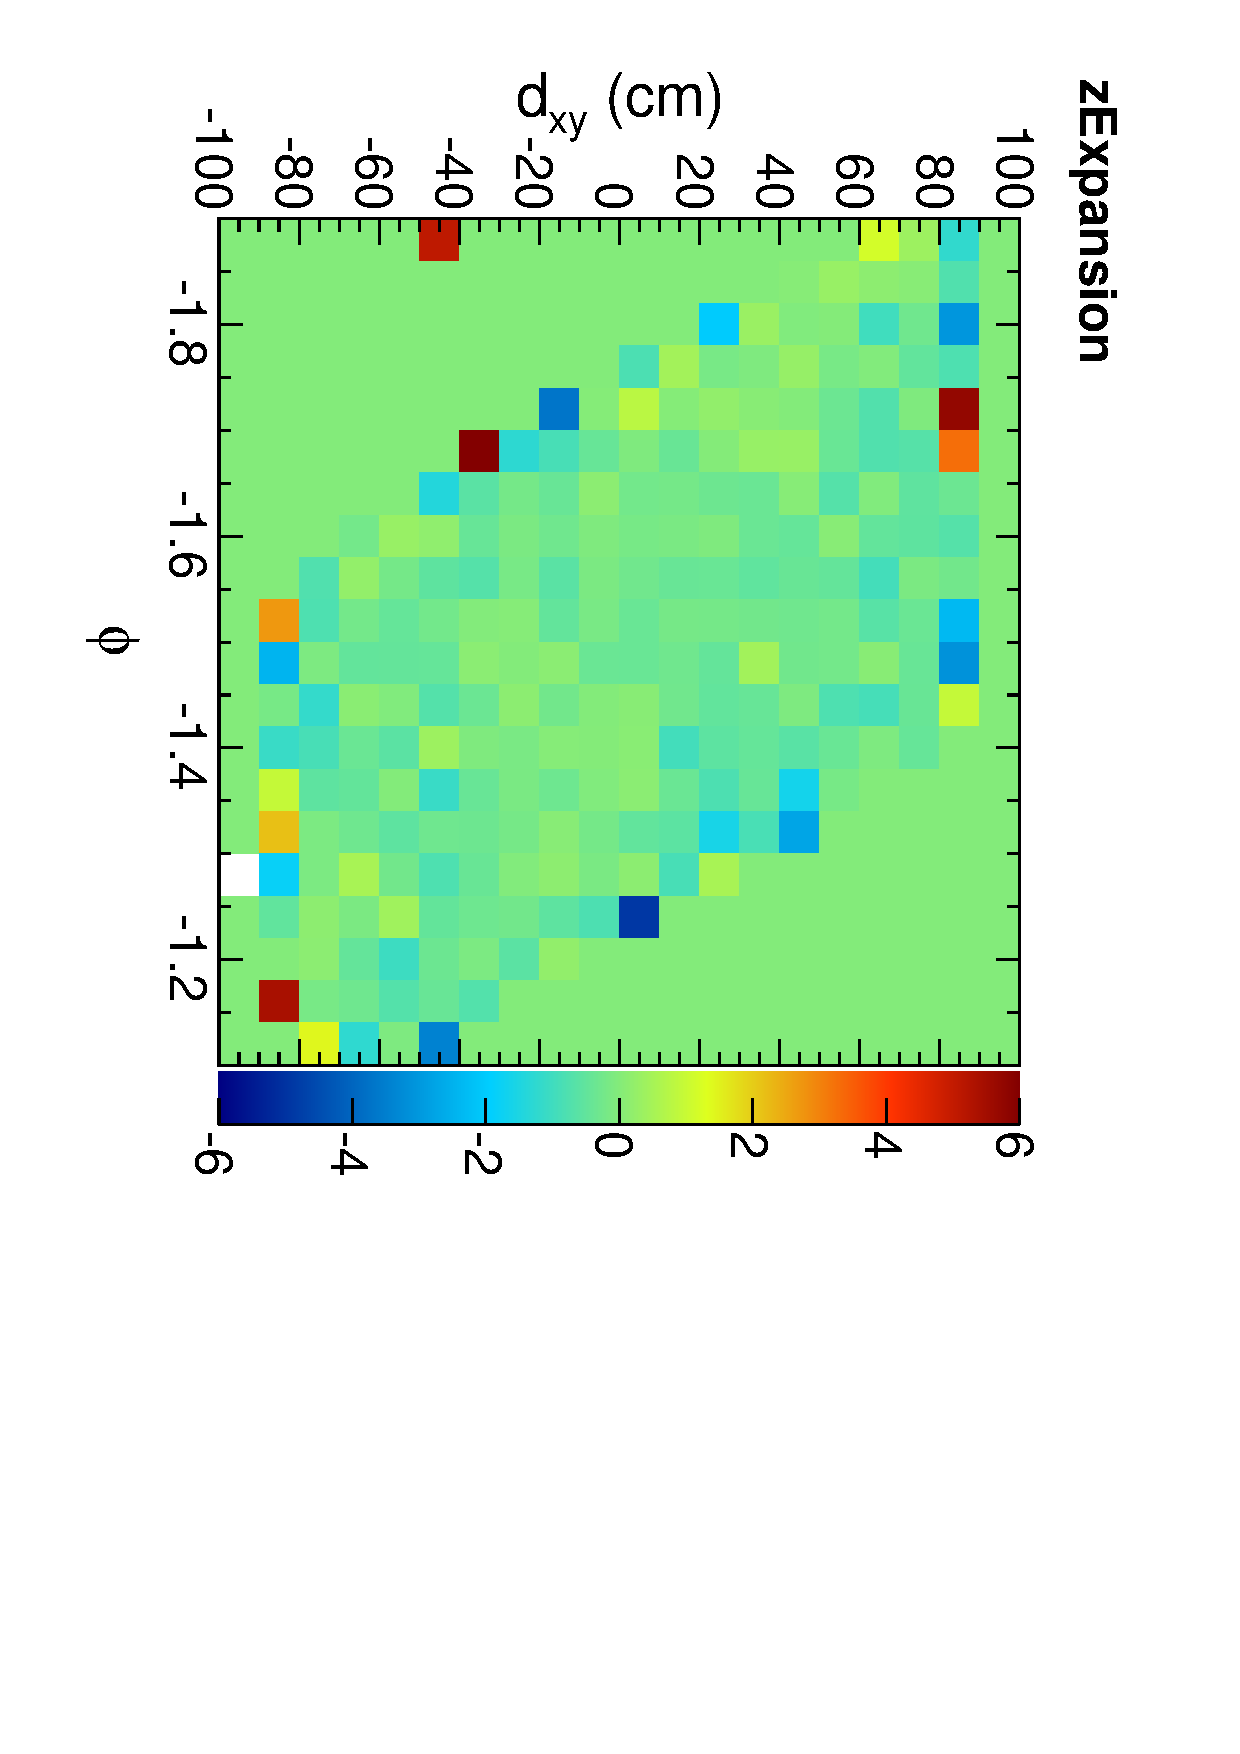
\includegraphics[height=0.32\linewidth, angle=90]{residx-dxy-phi-high_zExpansion.pdf}
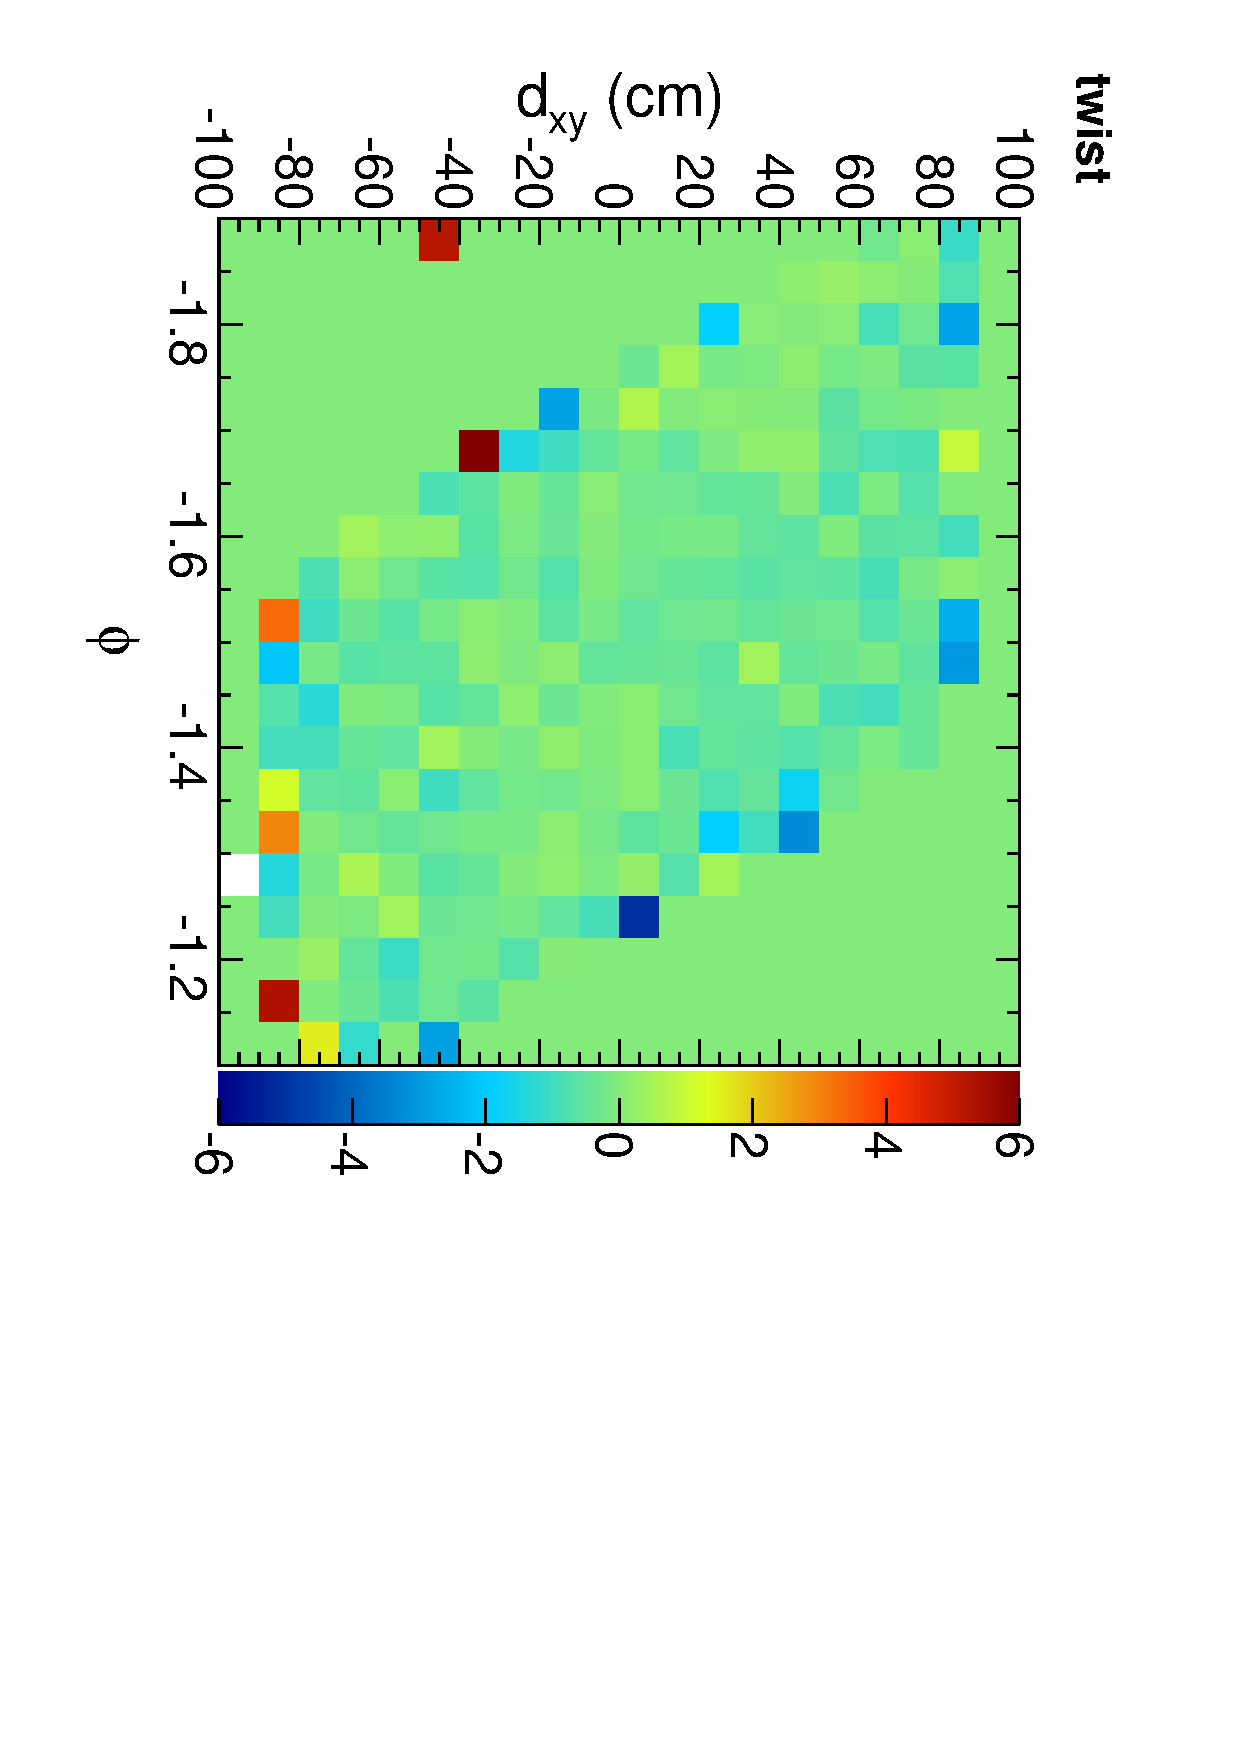
\includegraphics[height=0.32\linewidth, angle=90]{residx-dxy-phi-high_twist.pdf}

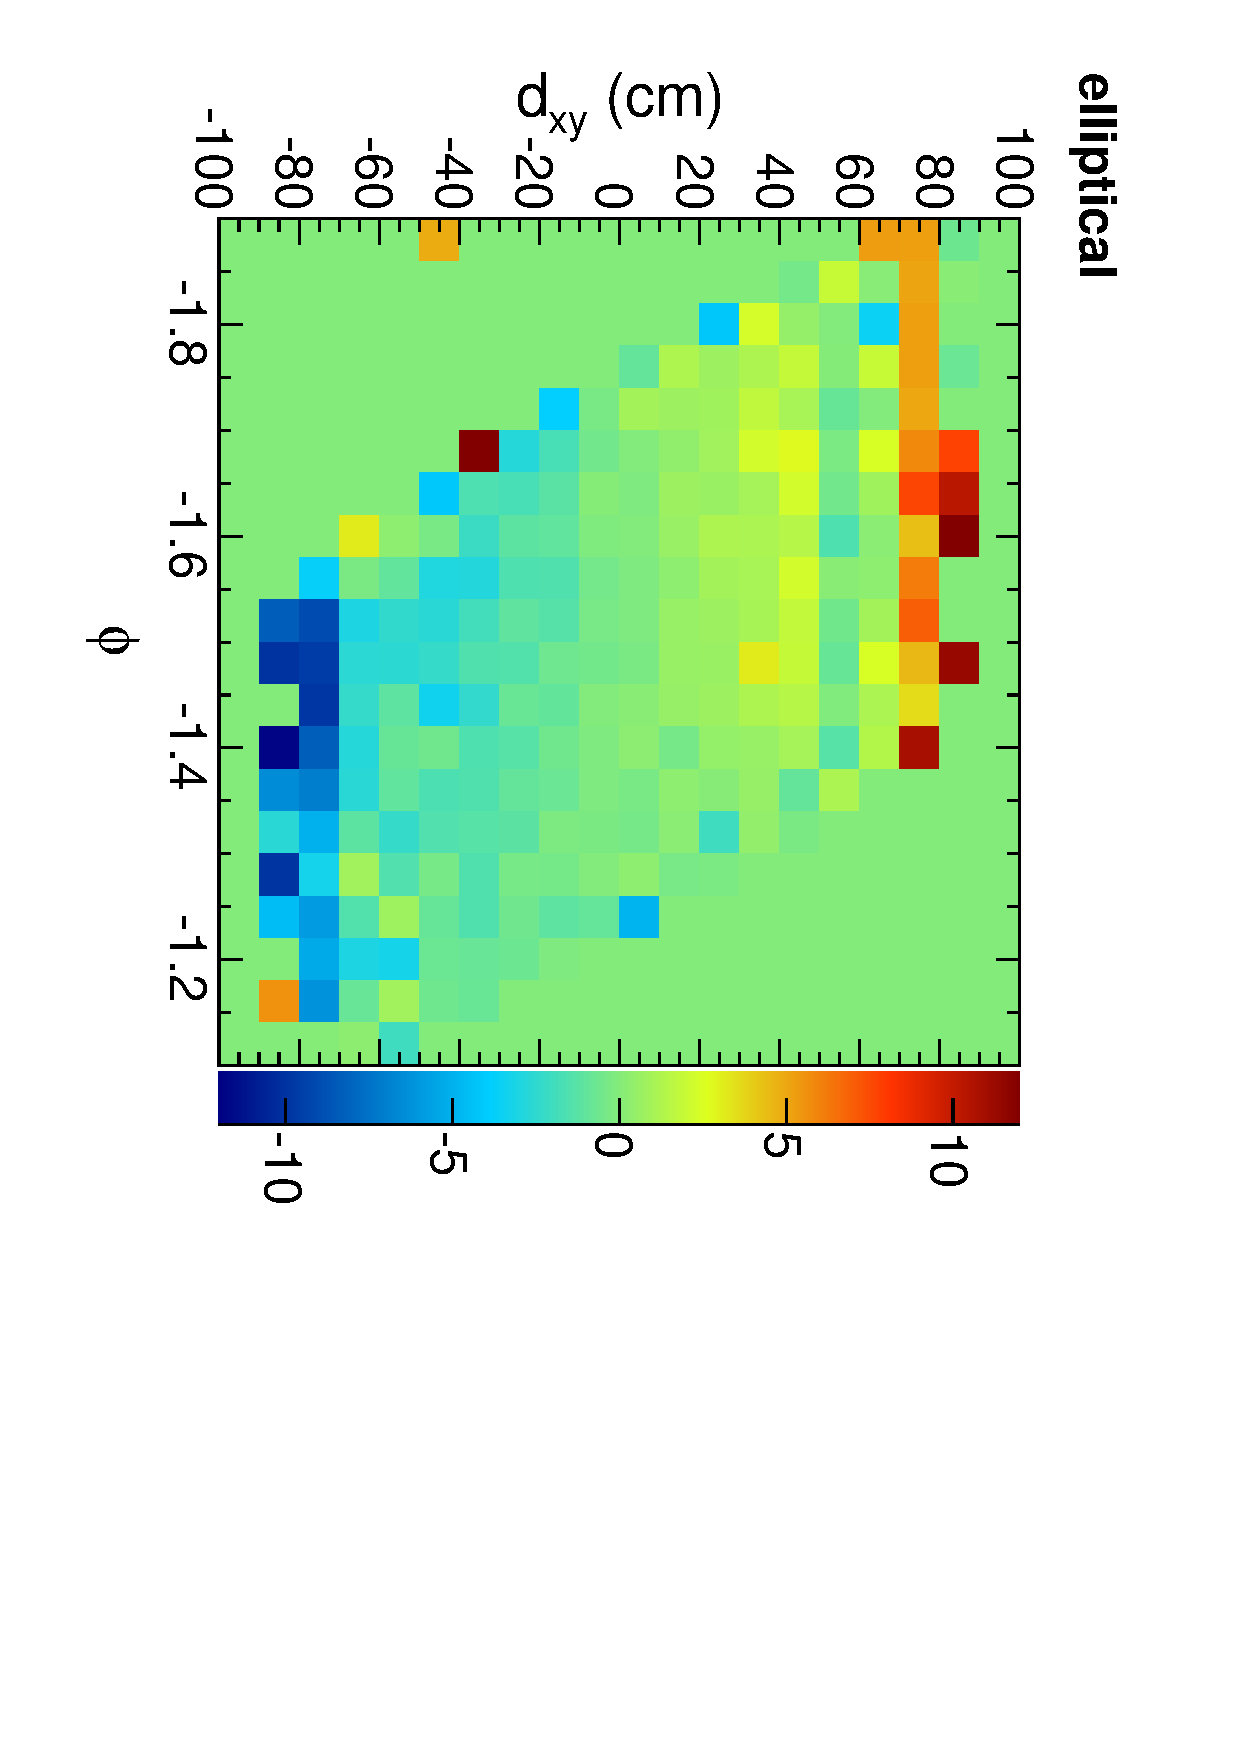
\includegraphics[height=0.32\linewidth, angle=90]{residx-dxy-phi-high_elliptical.pdf}
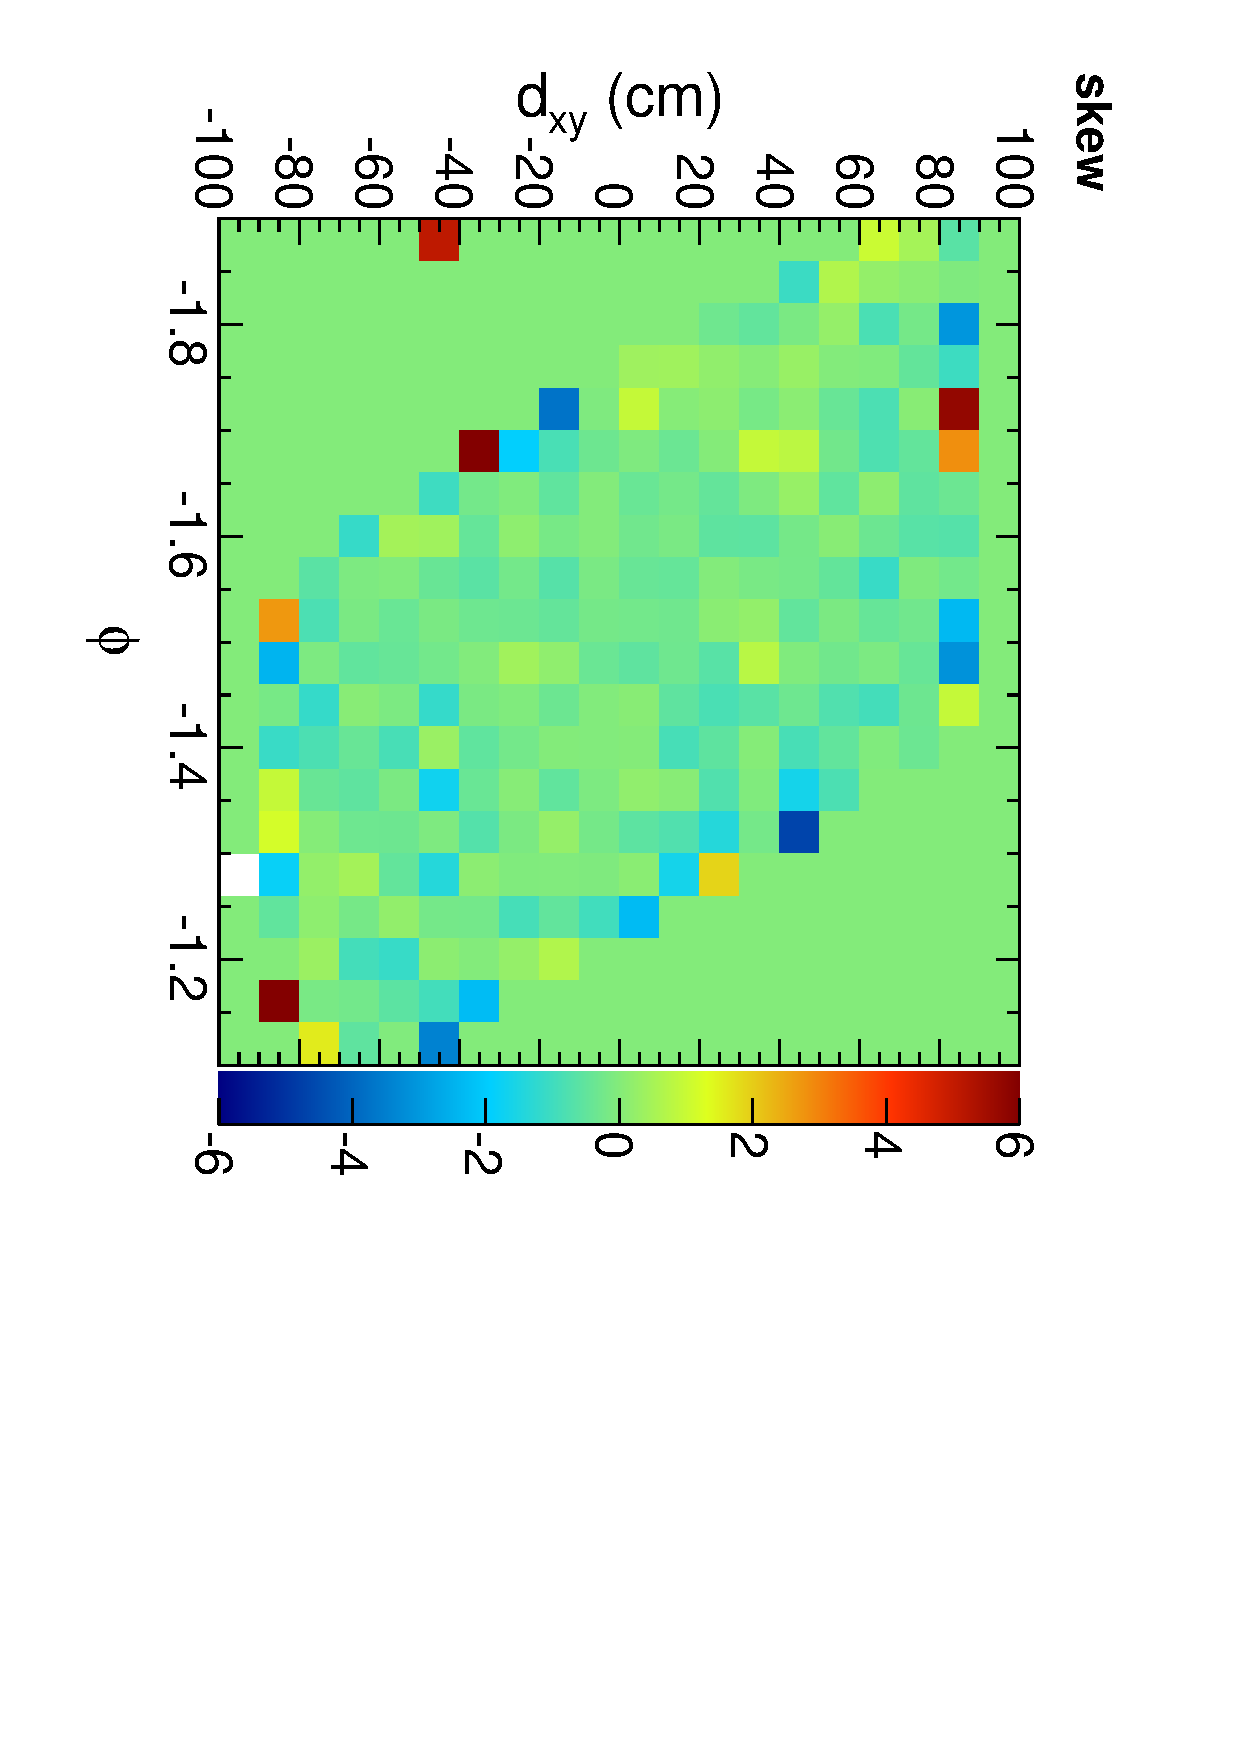
\includegraphics[height=0.32\linewidth, angle=90]{residx-dxy-phi-high_skew.pdf}
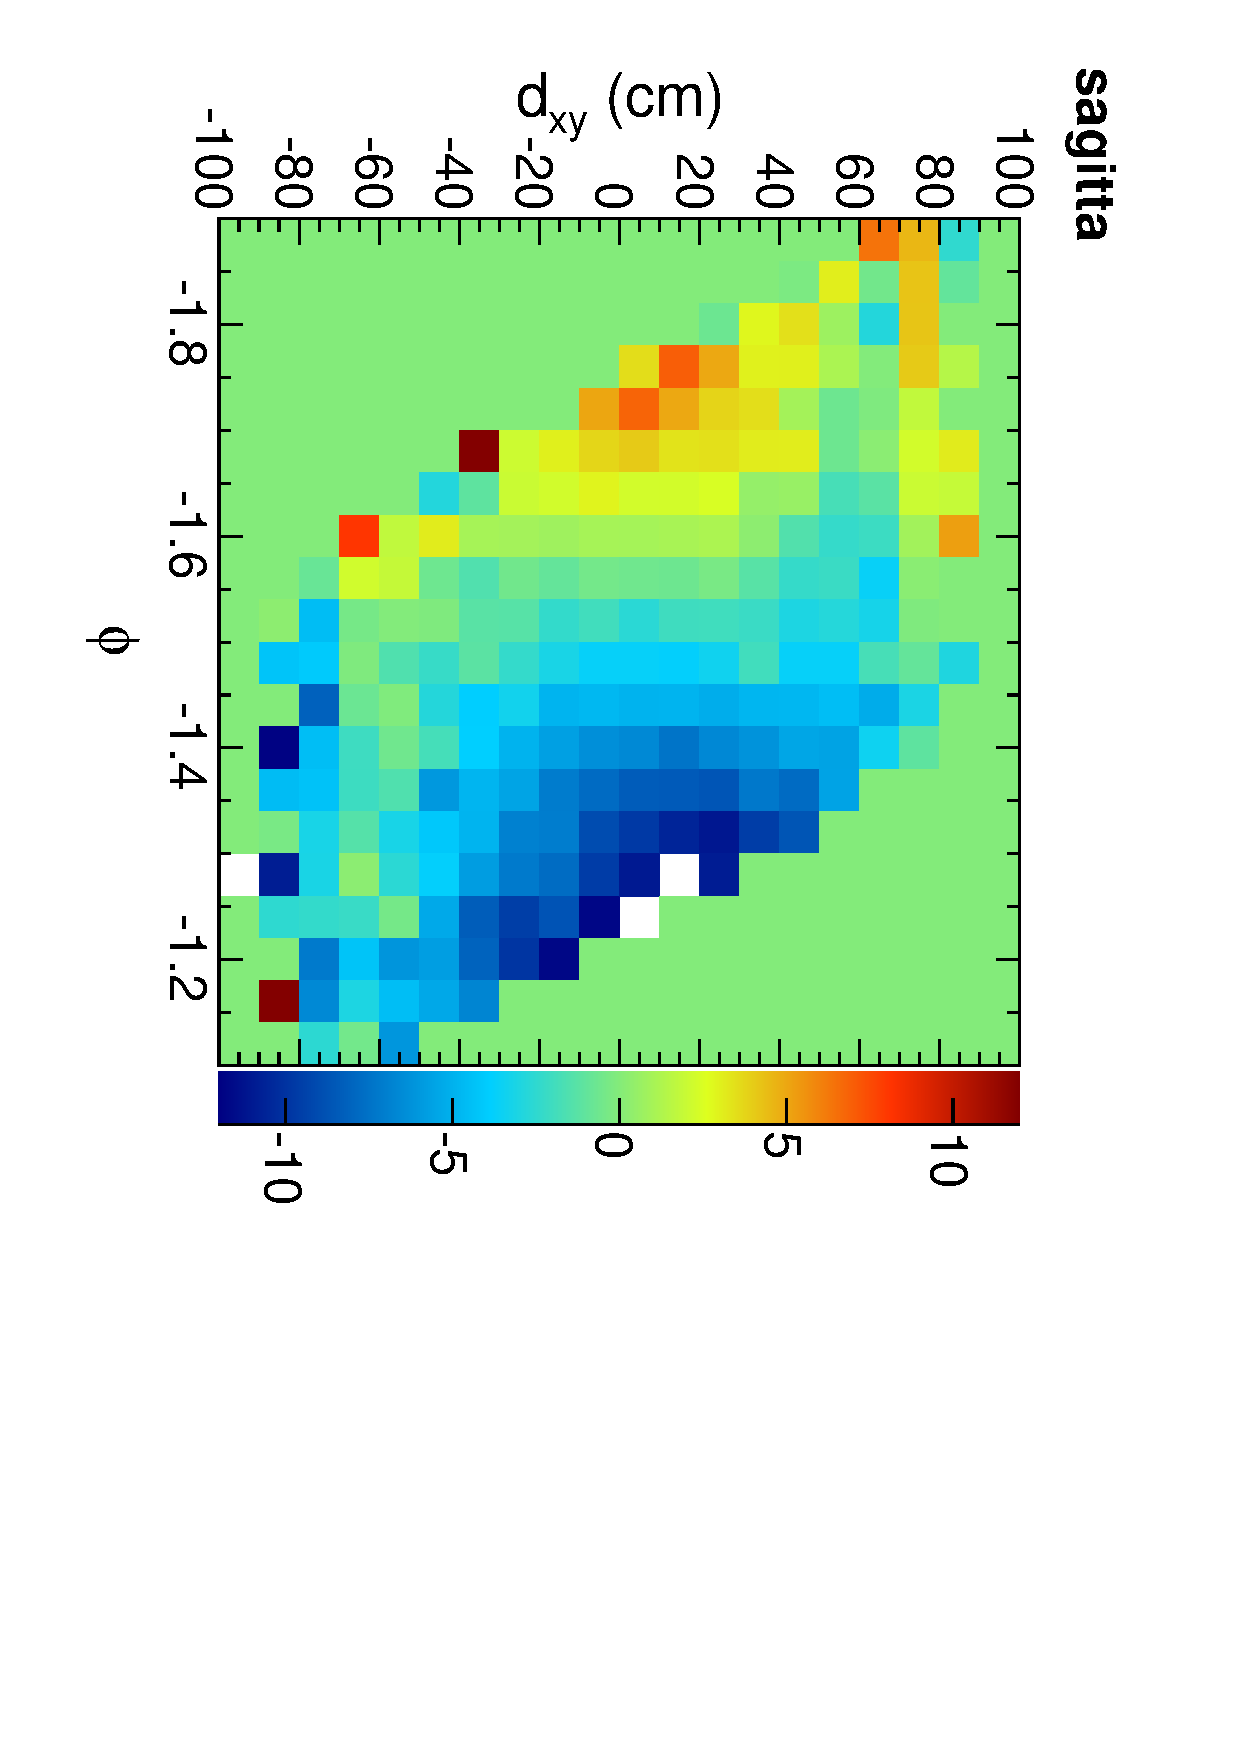
\includegraphics[height=0.32\linewidth, angle=90]{residx-dxy-phi-high_sagitta.pdf}
\end{columns}
\end{frame}

\begin{frame}
\frametitle{Residual vs.~$d_{xy}$ and $\phi$ (low $p_T$)}

\begin{itemize}
\item ``Low $p_T$'' means $p_T < 100$~GeV
\item This is a simple pattern: does it suggest a geometric interpretation?
\end{itemize}

\begin{columns}
\column{0.4\linewidth}
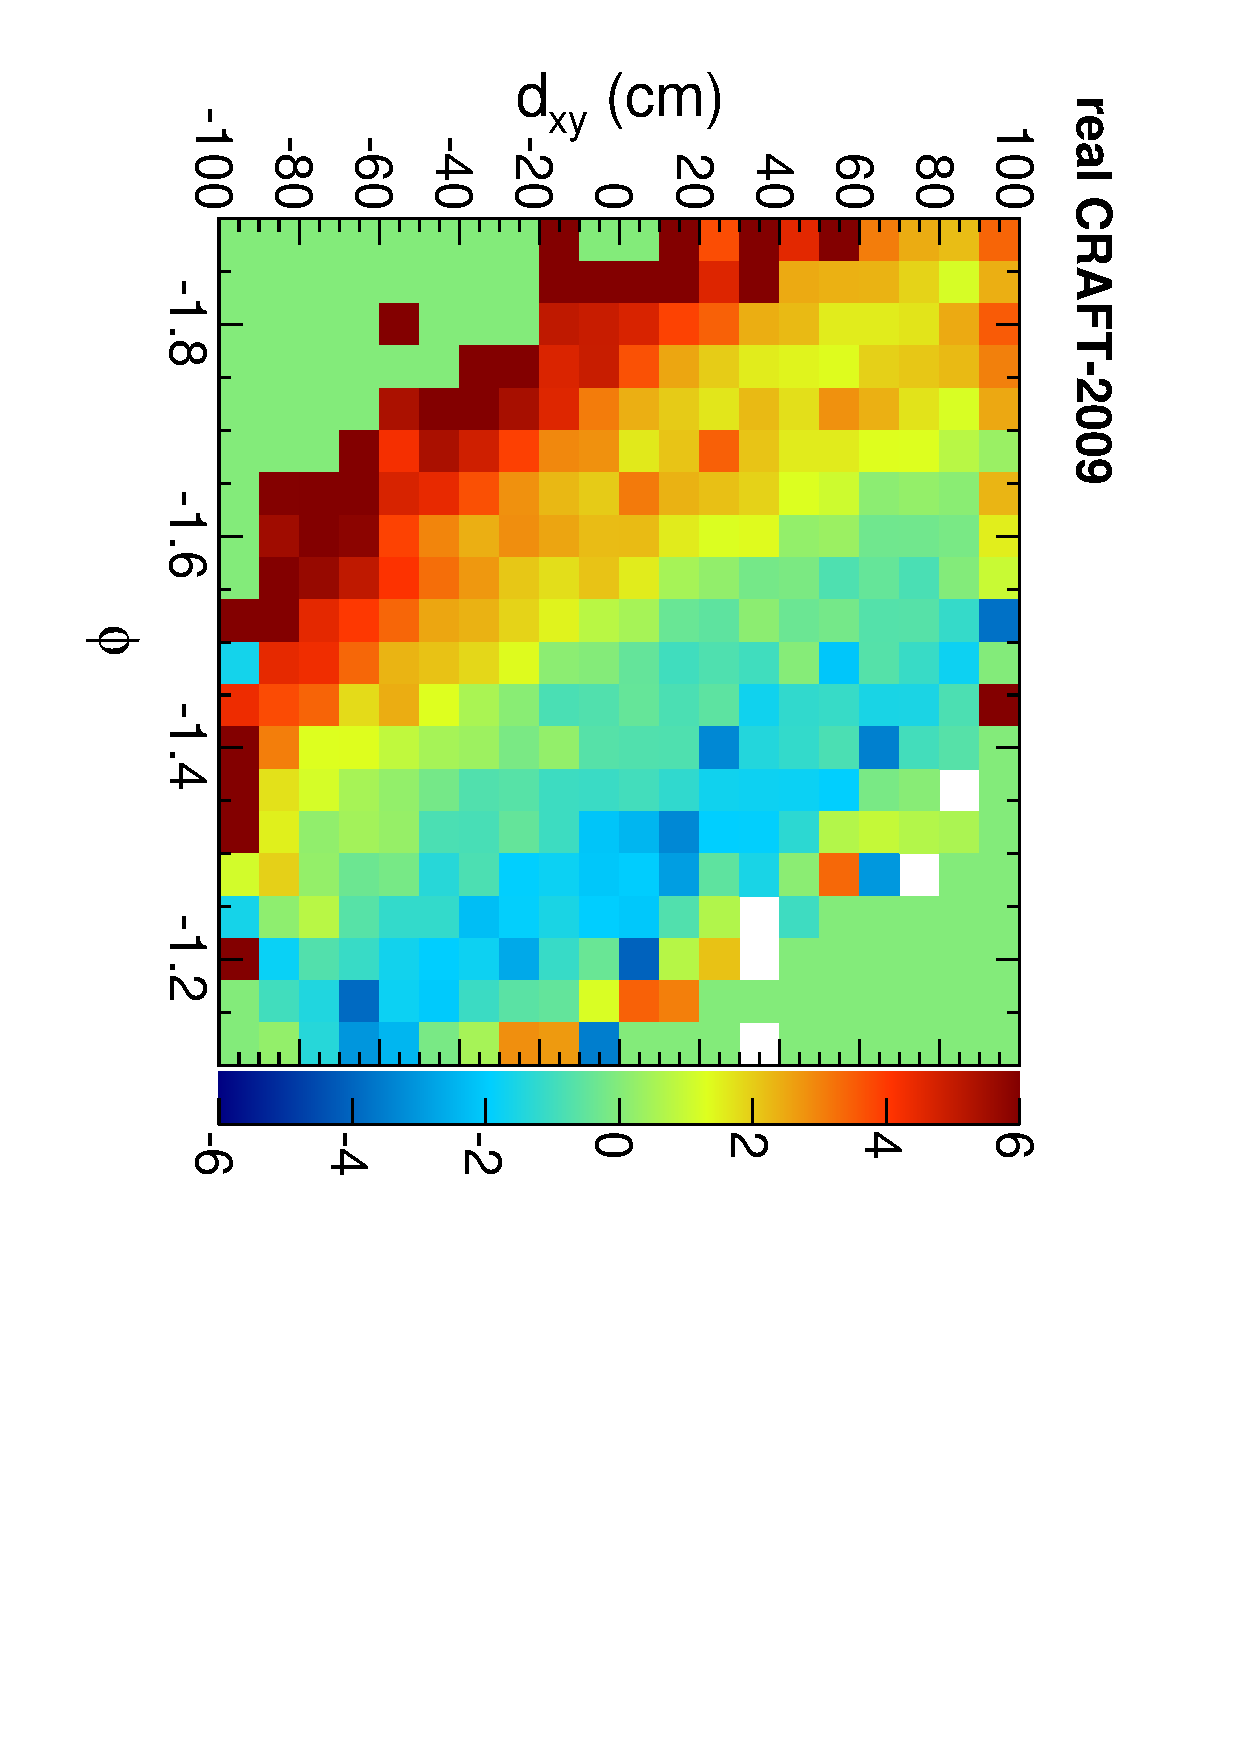
\includegraphics[height=\linewidth, angle=90]{residx-dxy-phi-low_real.pdf}

\column{0.6\linewidth}
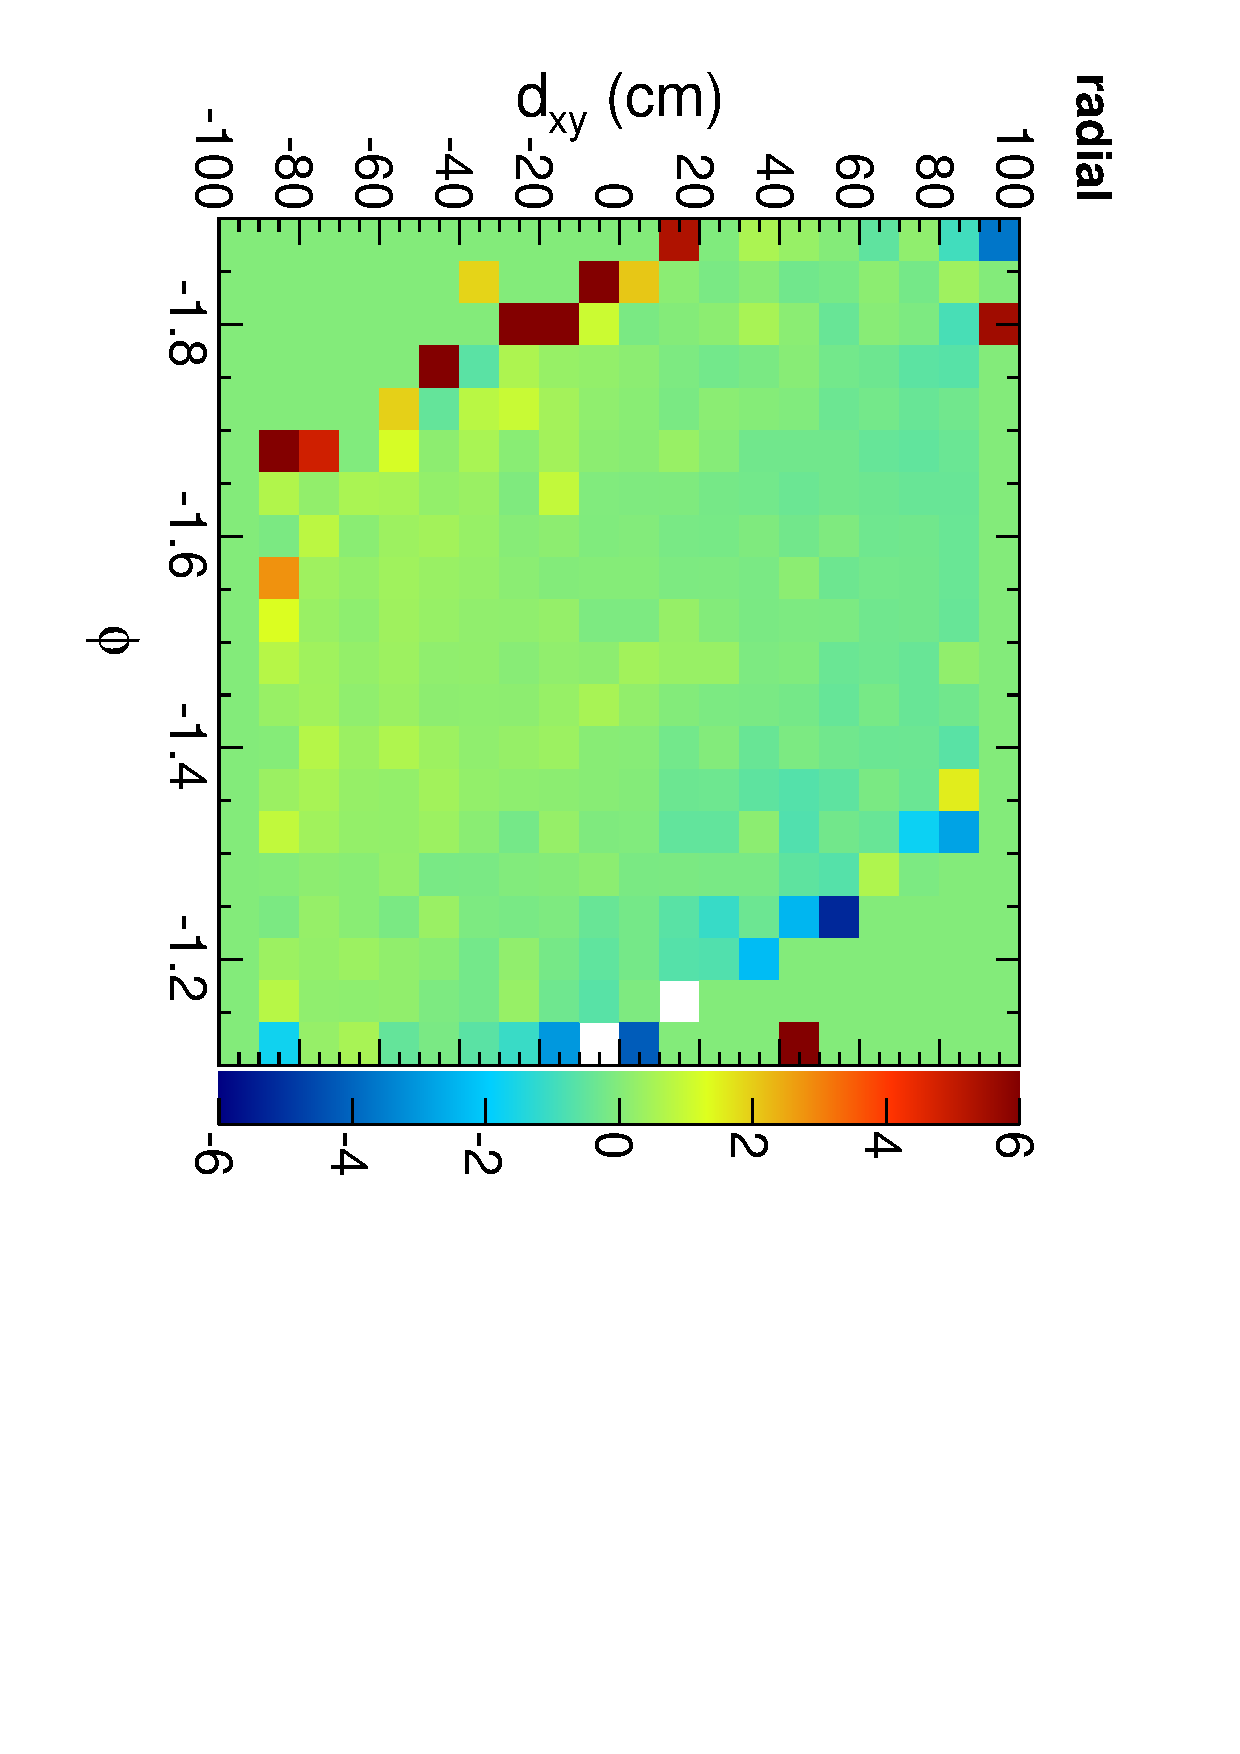
\includegraphics[height=0.32\linewidth, angle=90]{residx-dxy-phi-low_radial.pdf}
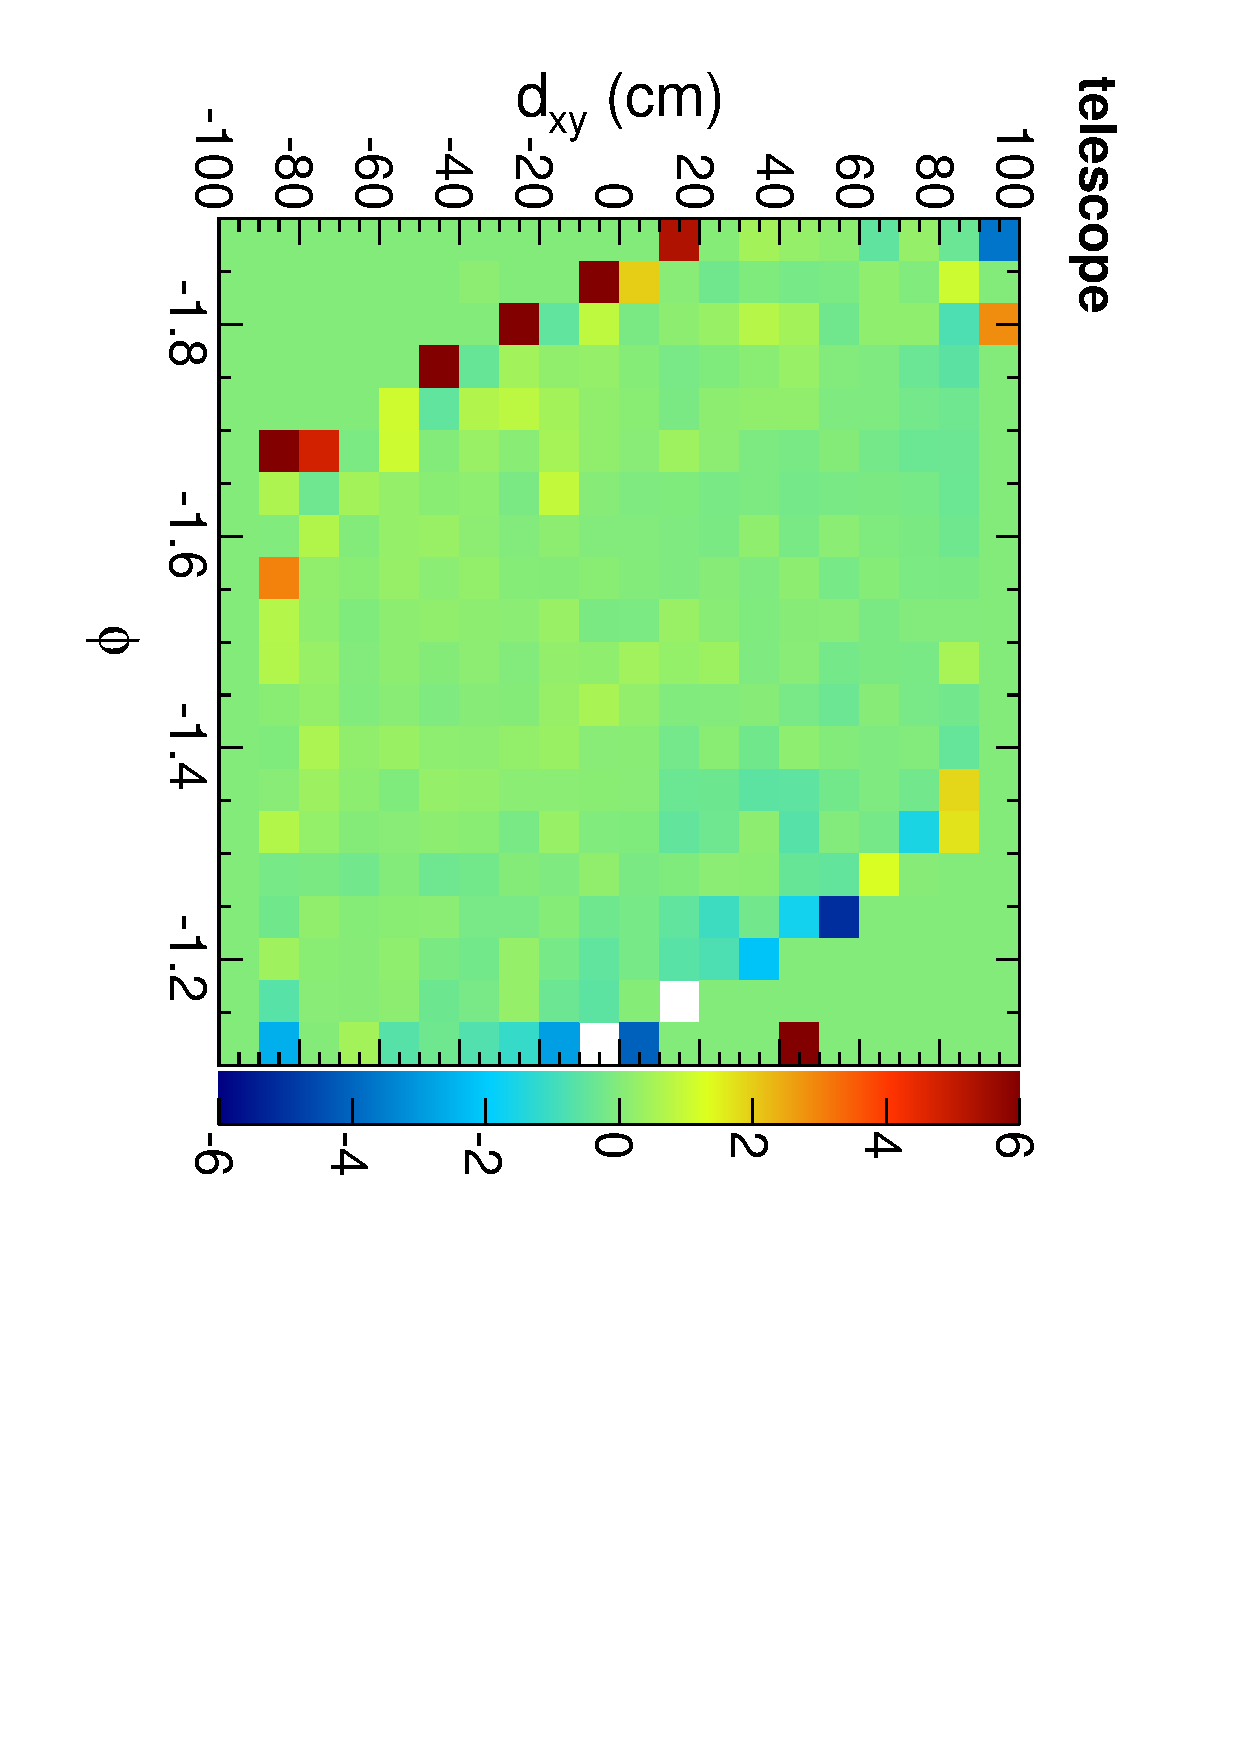
\includegraphics[height=0.32\linewidth, angle=90]{residx-dxy-phi-low_telescope.pdf}
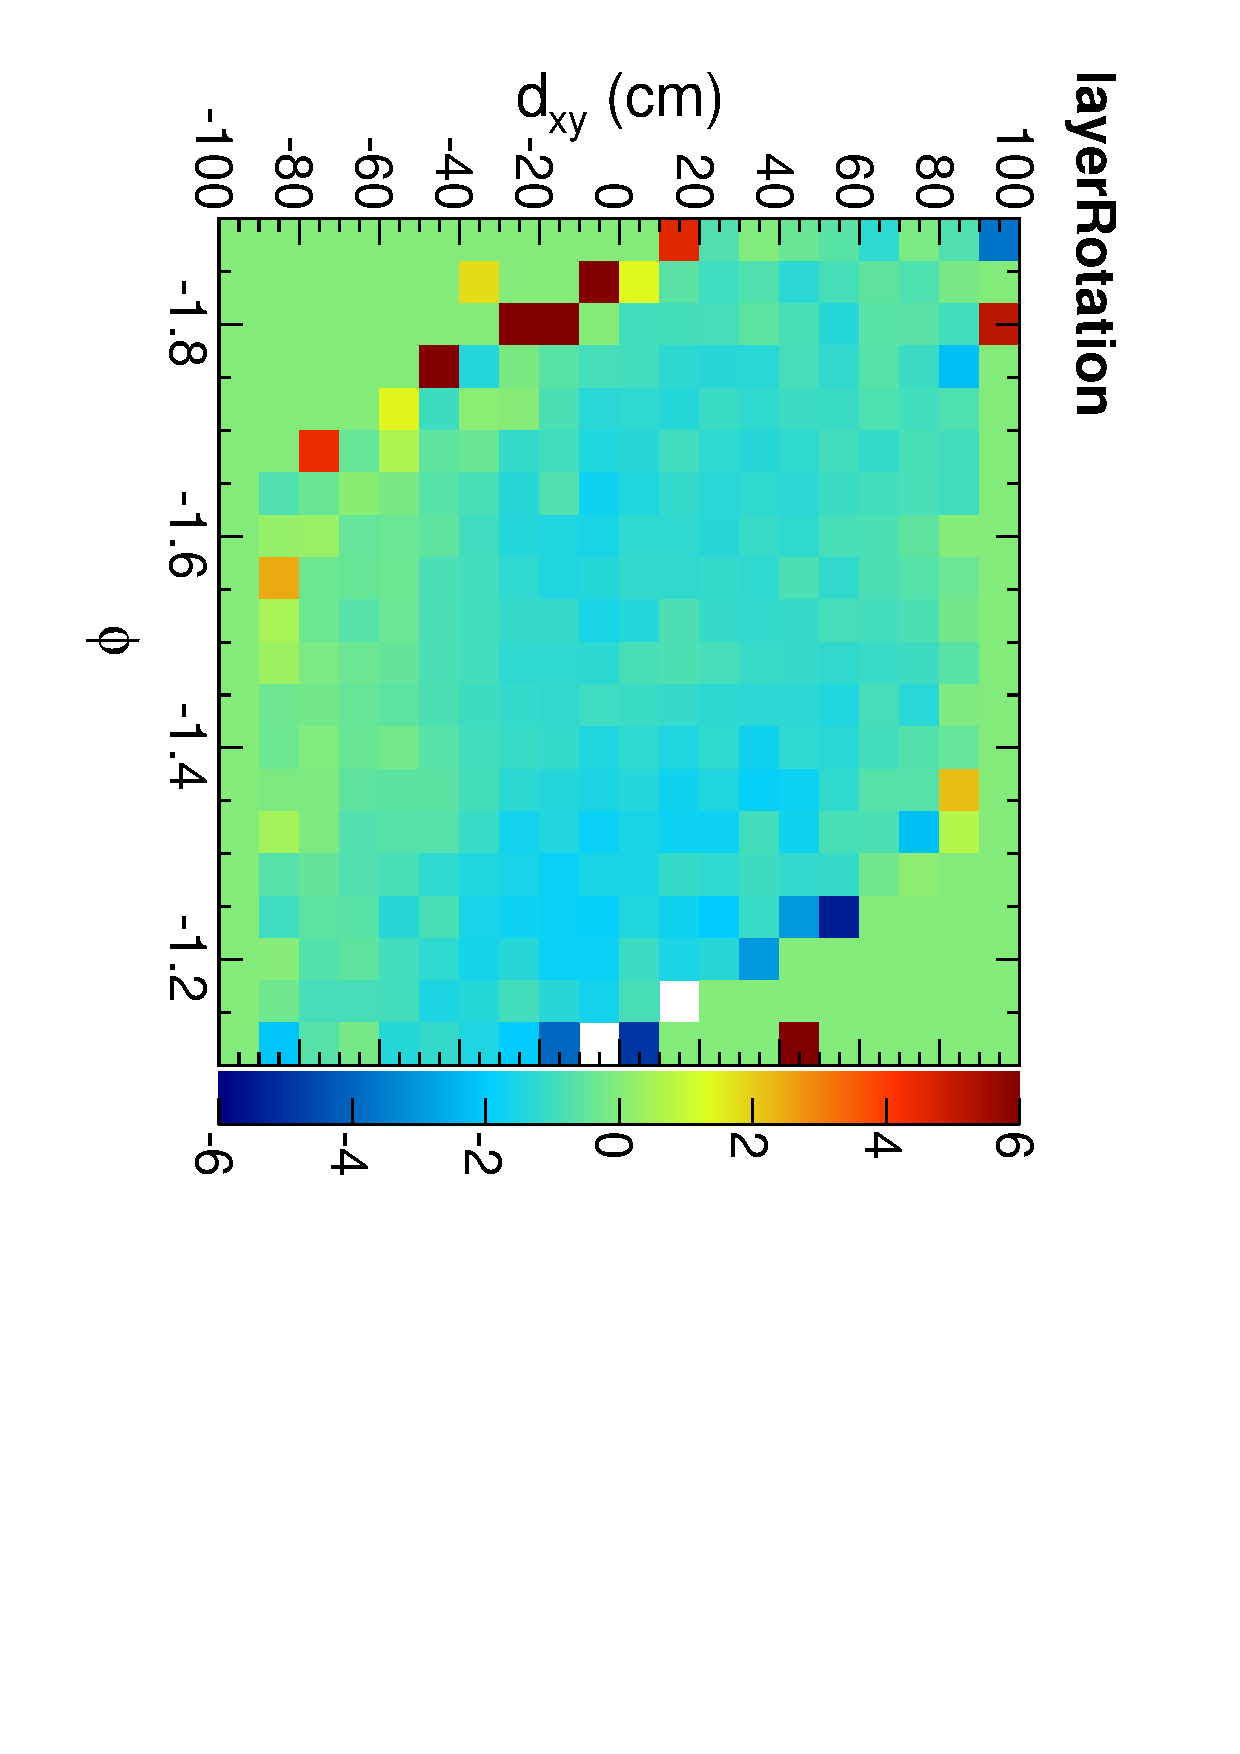
\includegraphics[height=0.32\linewidth, angle=90]{residx-dxy-phi-low_layerRotation.pdf}

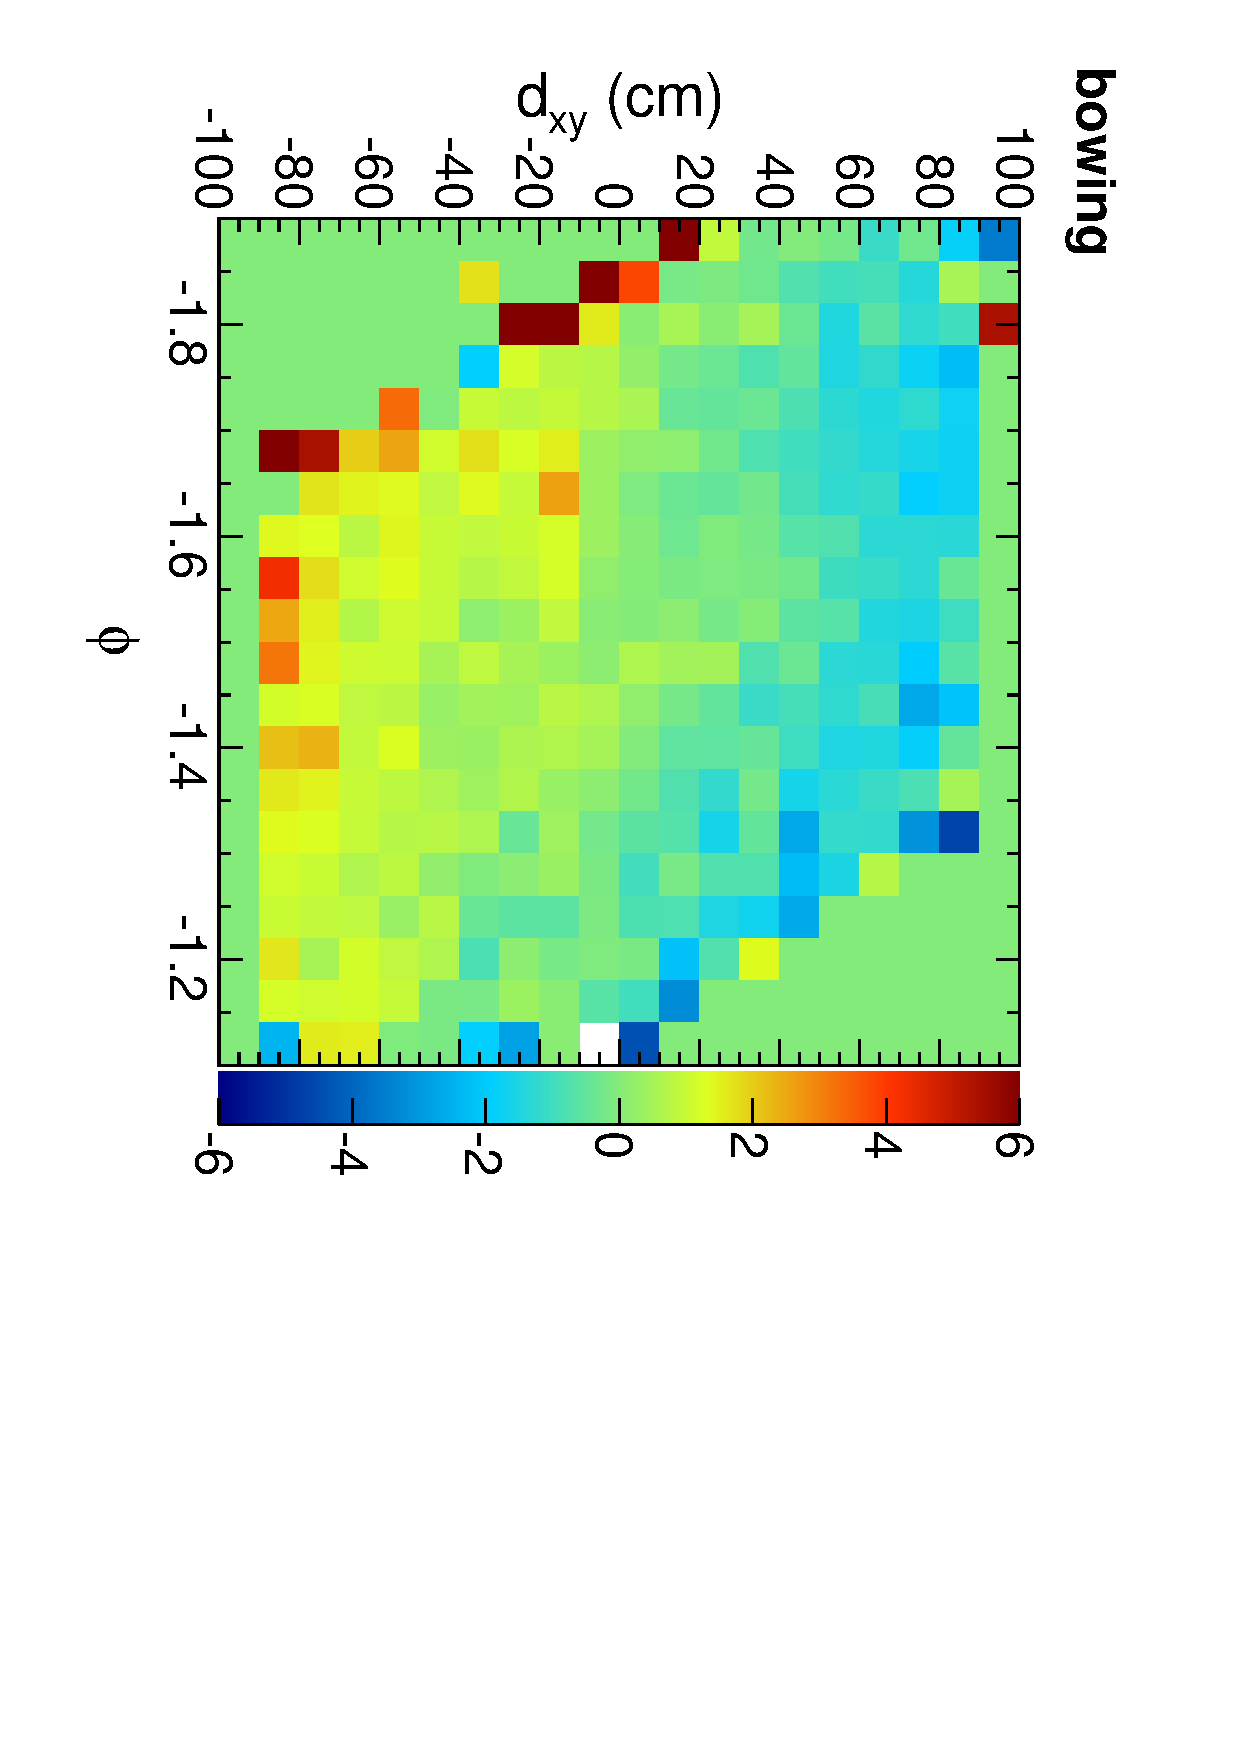
\includegraphics[height=0.32\linewidth, angle=90]{residx-dxy-phi-low_bowing.pdf}
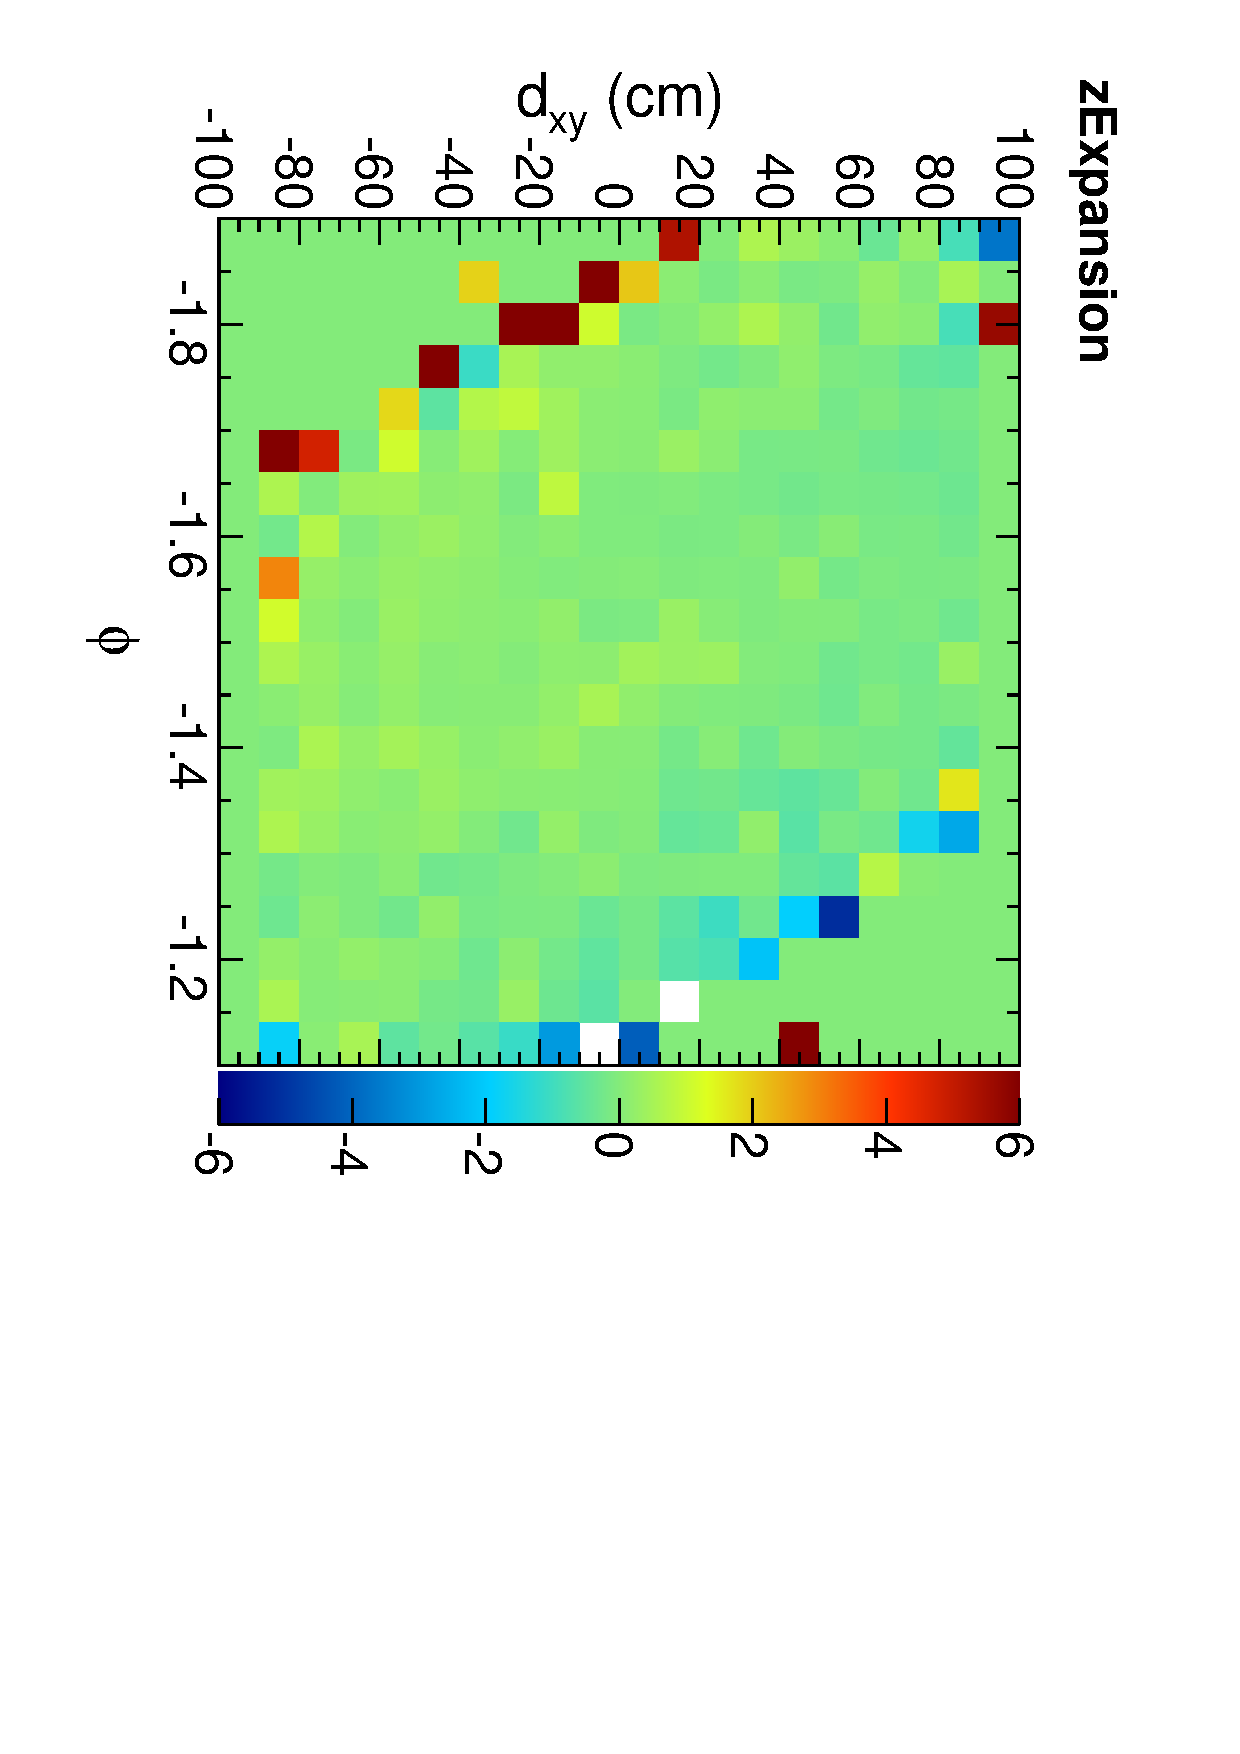
\includegraphics[height=0.32\linewidth, angle=90]{residx-dxy-phi-low_zExpansion.pdf}
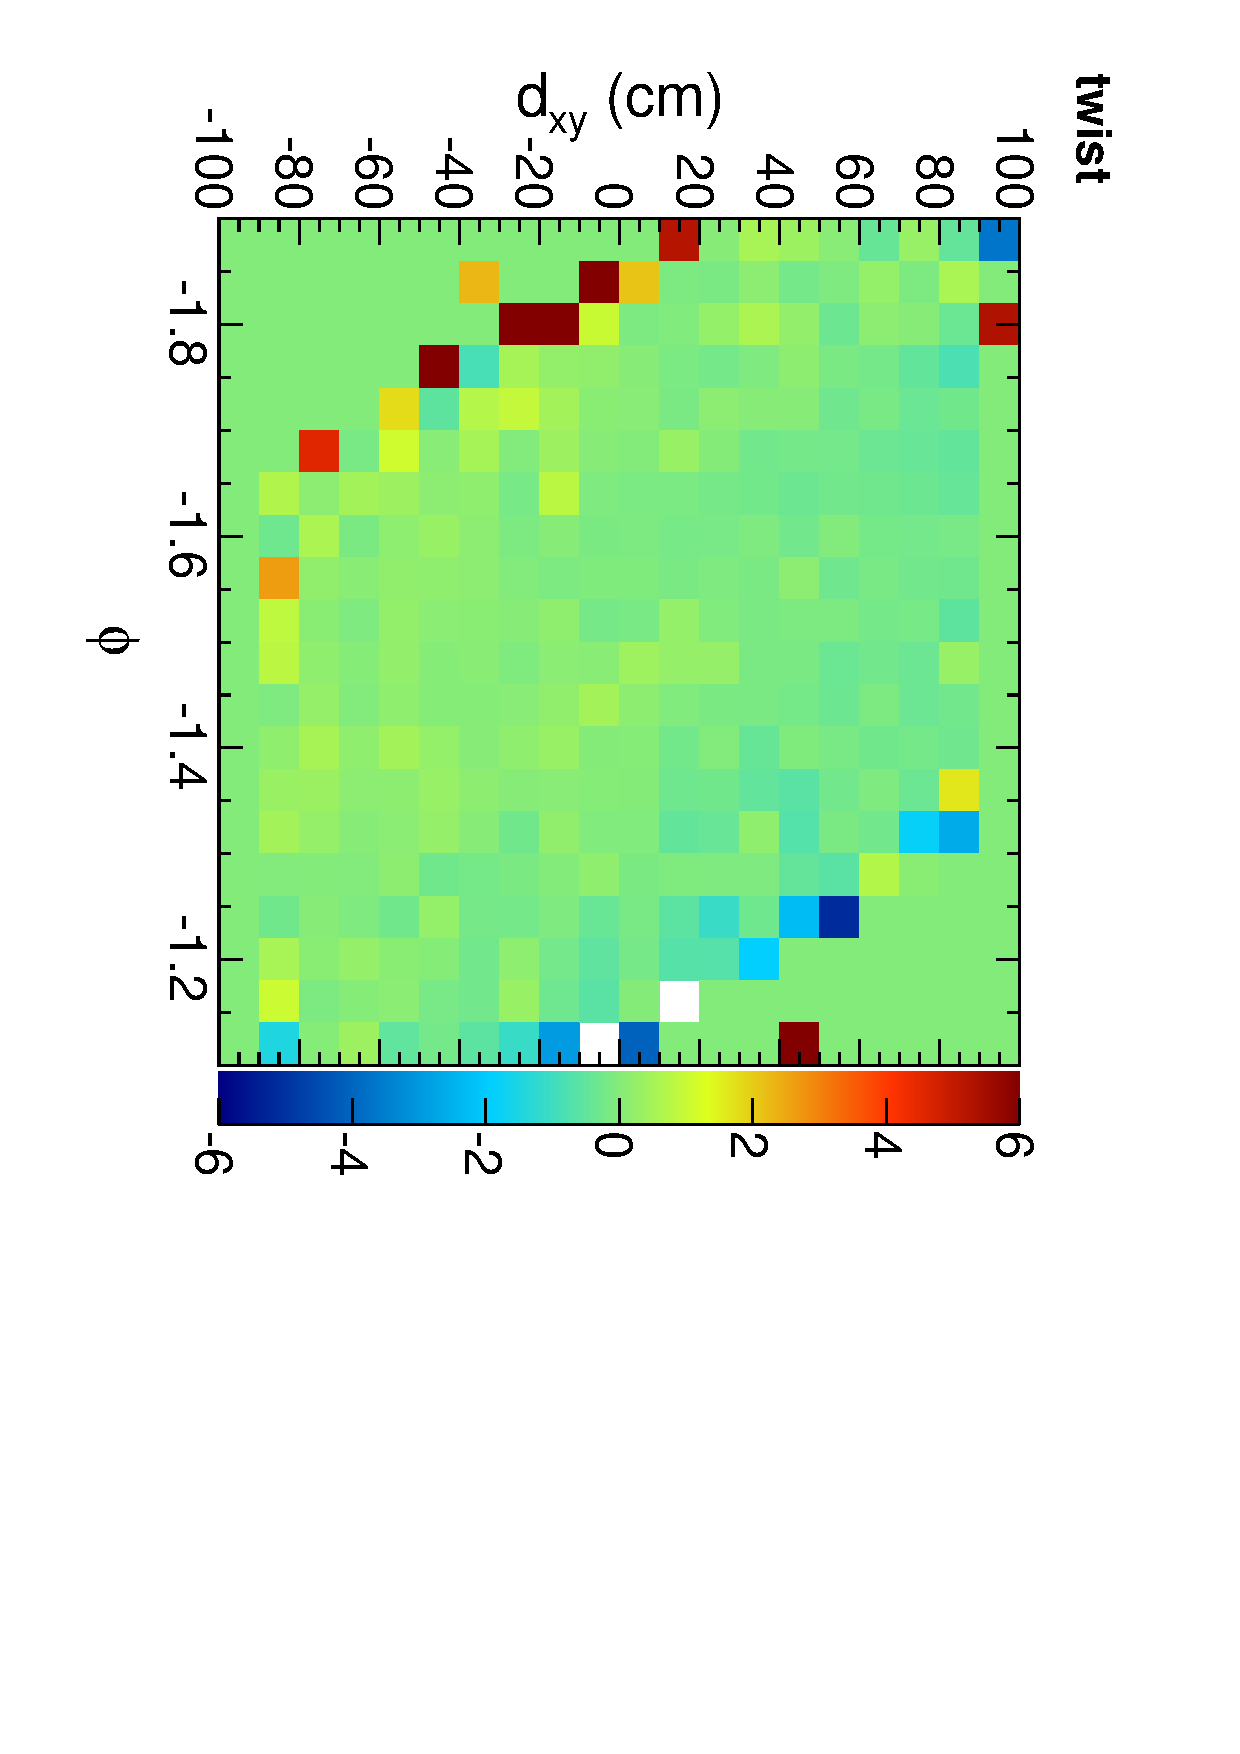
\includegraphics[height=0.32\linewidth, angle=90]{residx-dxy-phi-low_twist.pdf}

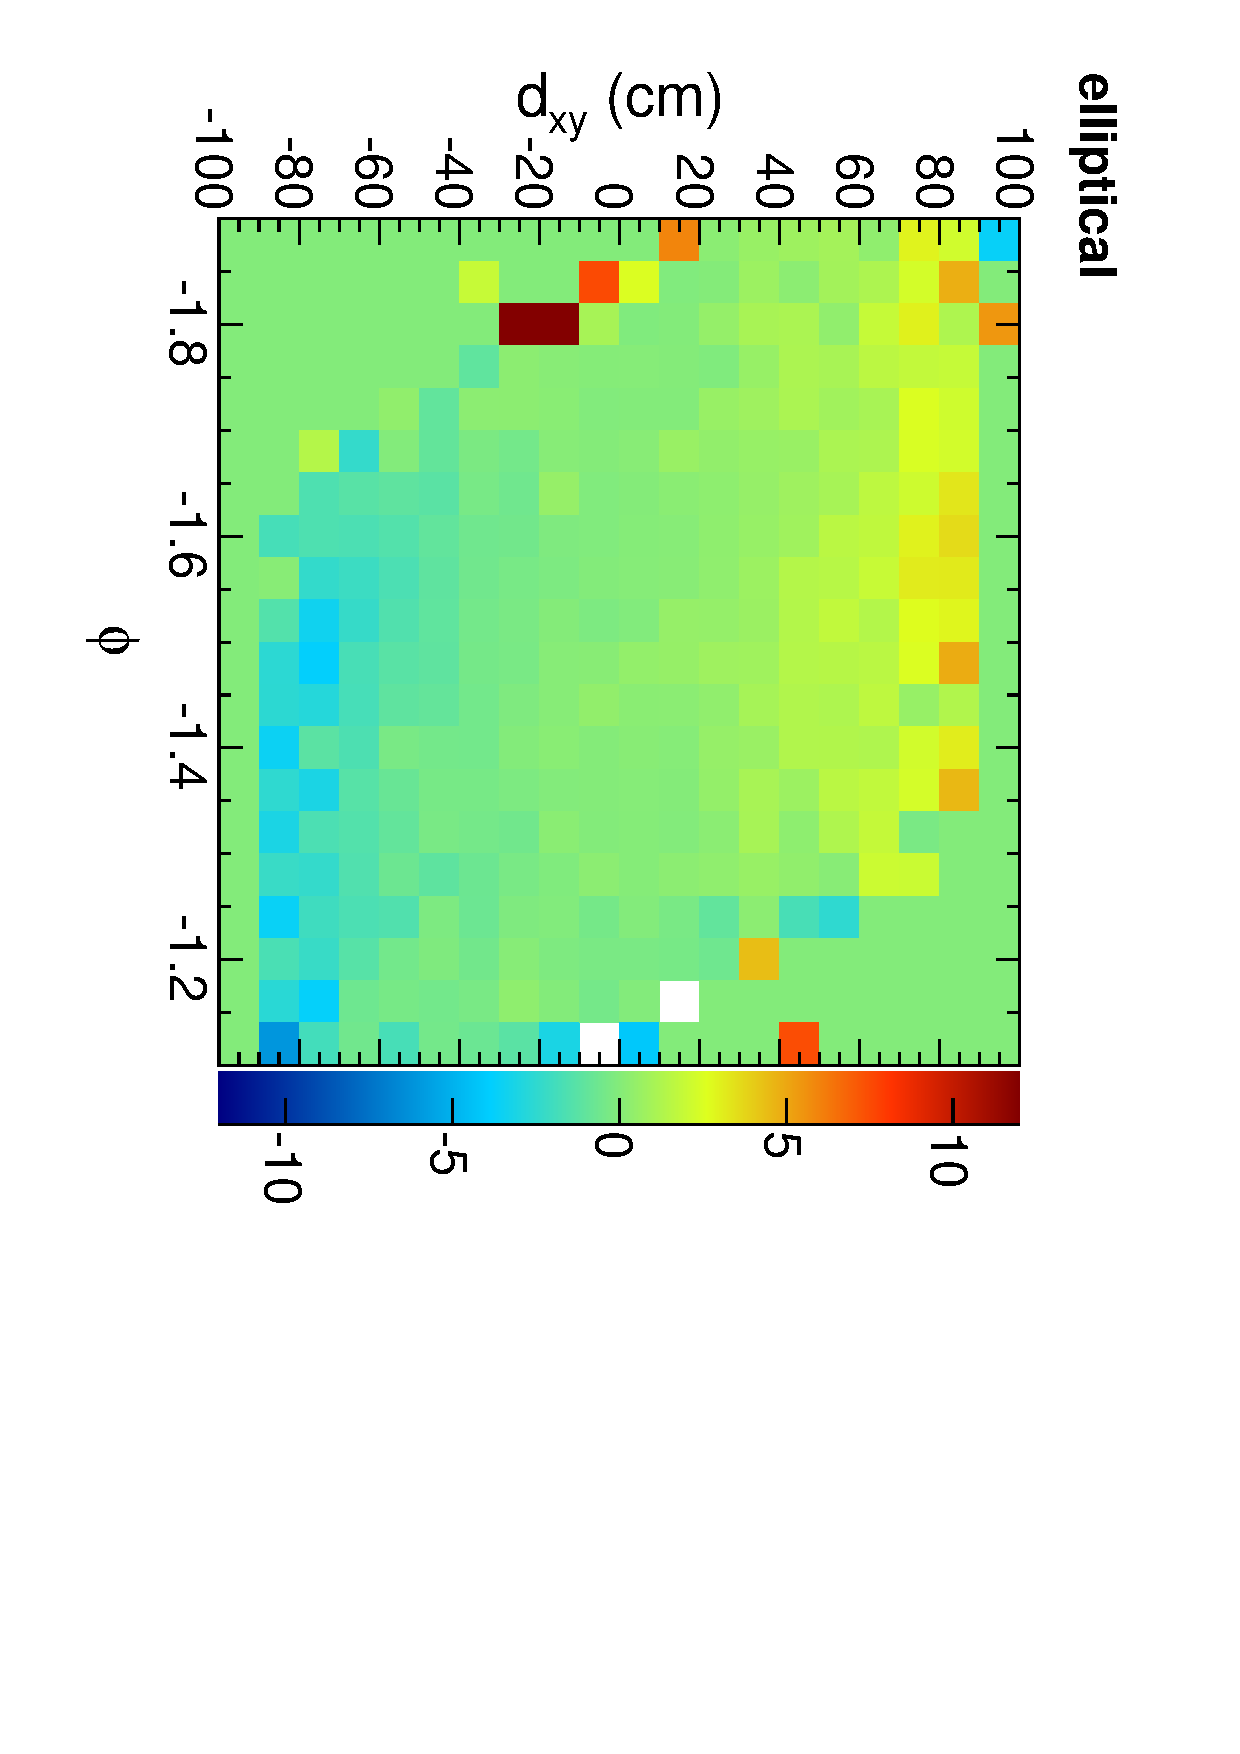
\includegraphics[height=0.32\linewidth, angle=90]{residx-dxy-phi-low_elliptical.pdf}
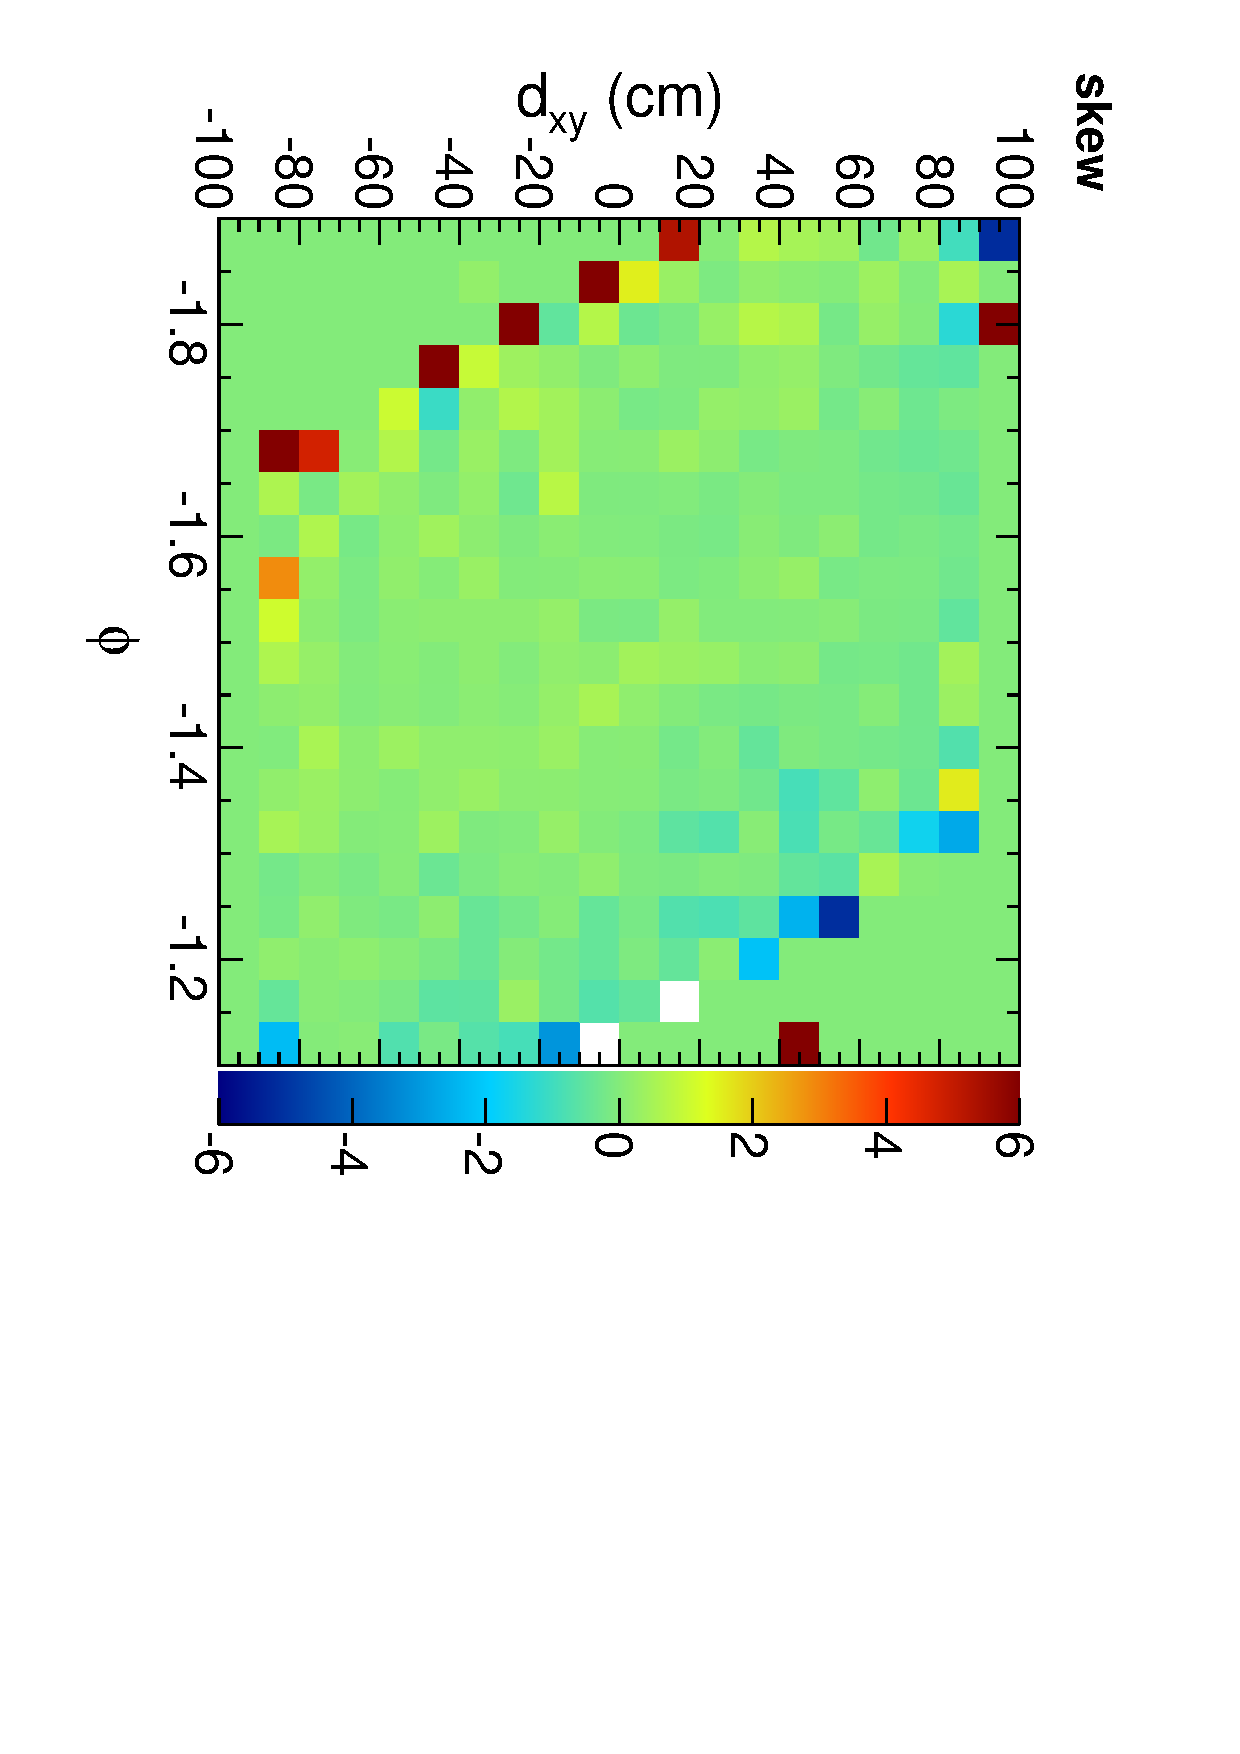
\includegraphics[height=0.32\linewidth, angle=90]{residx-dxy-phi-low_skew.pdf}
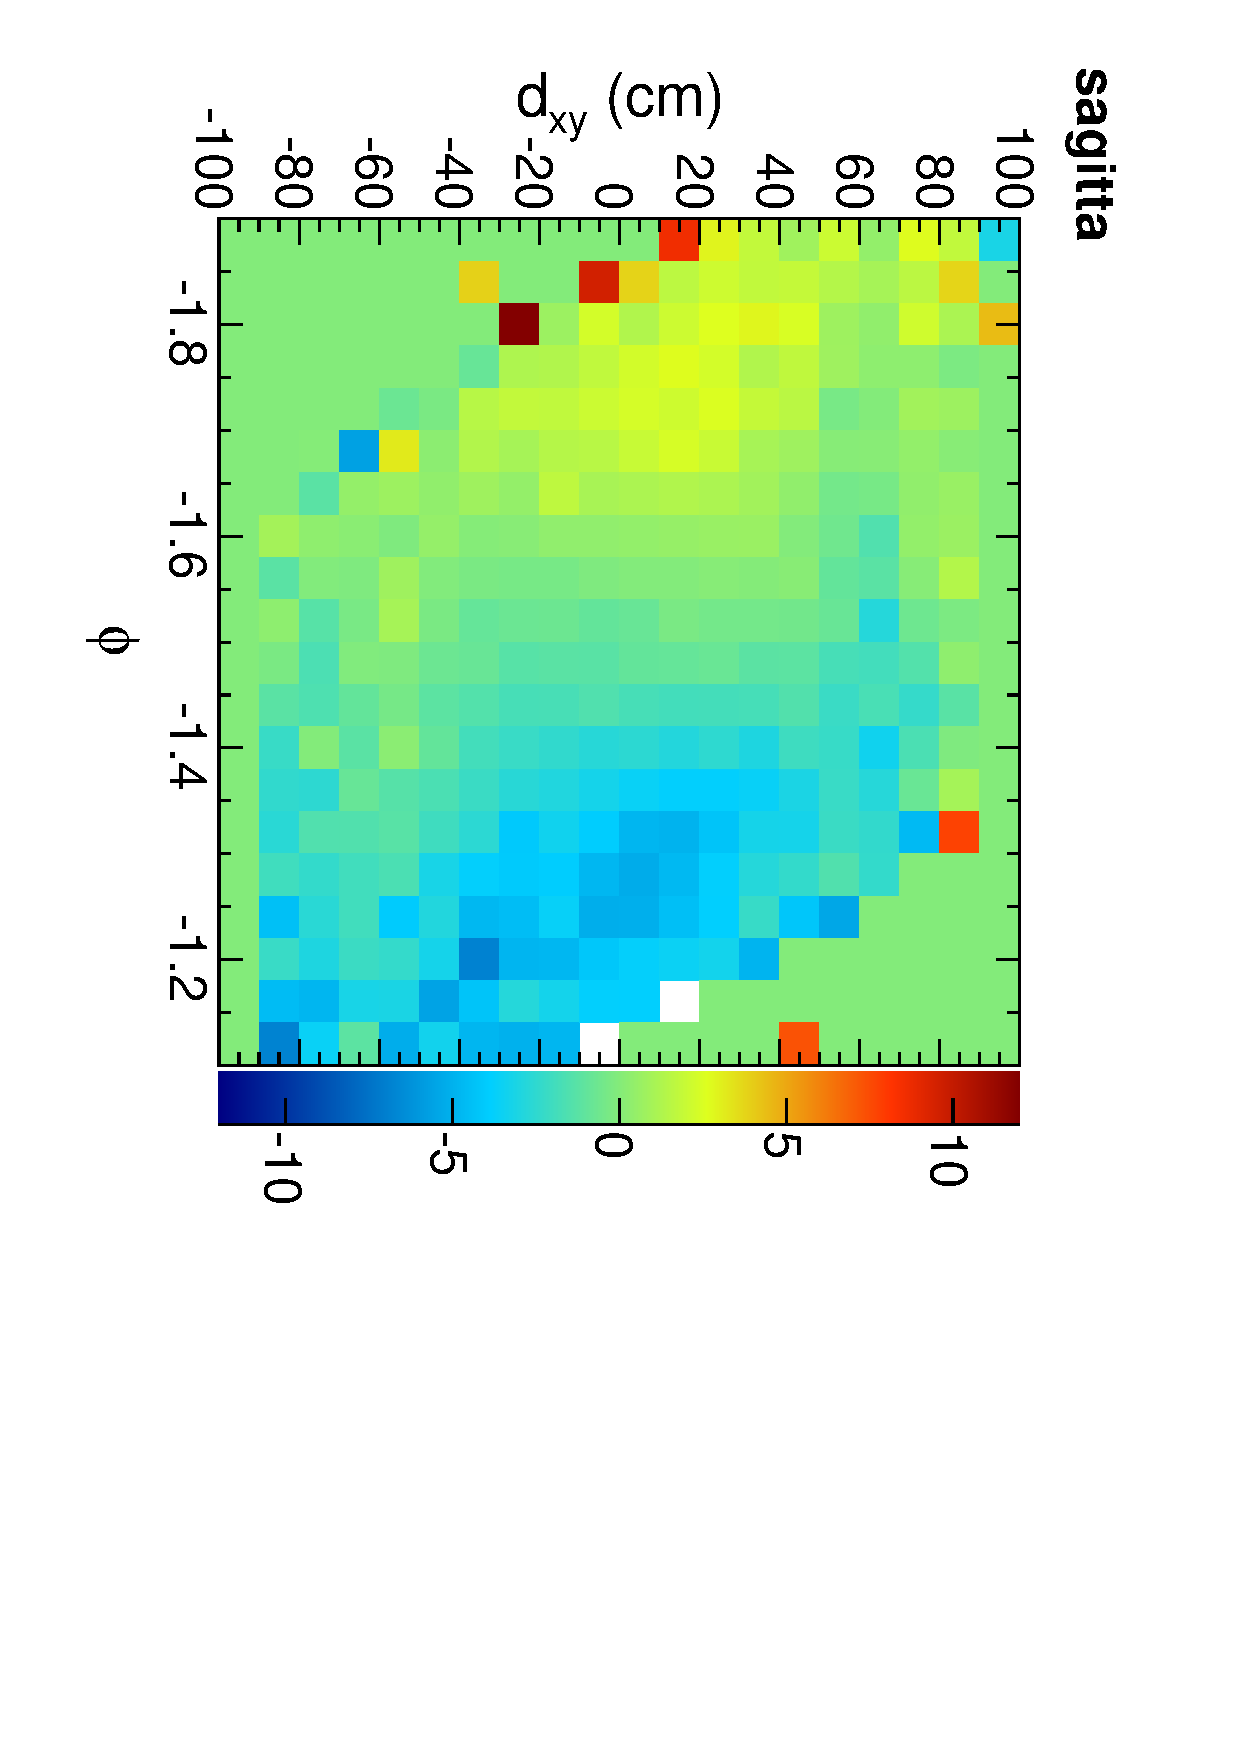
\includegraphics[height=0.32\linewidth, angle=90]{residx-dxy-phi-low_sagitta.pdf}
\end{columns}
\end{frame}

\begin{frame}
\frametitle{Clue from MC study}

\begin{itemize}
\item When we conducted the MC cosmic ray alignment exercise, the
  combined system acquired a global distortion resembling sagitta, too
\item Left: muon chamber $\phi$ positions relative to MC-truth, aligned using TrackerAlignment\_CRAFT08Realistic\_mc
\item Right: same thing for the 9 globally-distorted tracker modes
\begin{itemize}
\item at the extremes of the bottom-right plot, muon chamber misalignments were too large to recover, but the shape is $\cos\phi$
\end{itemize}
\end{itemize}

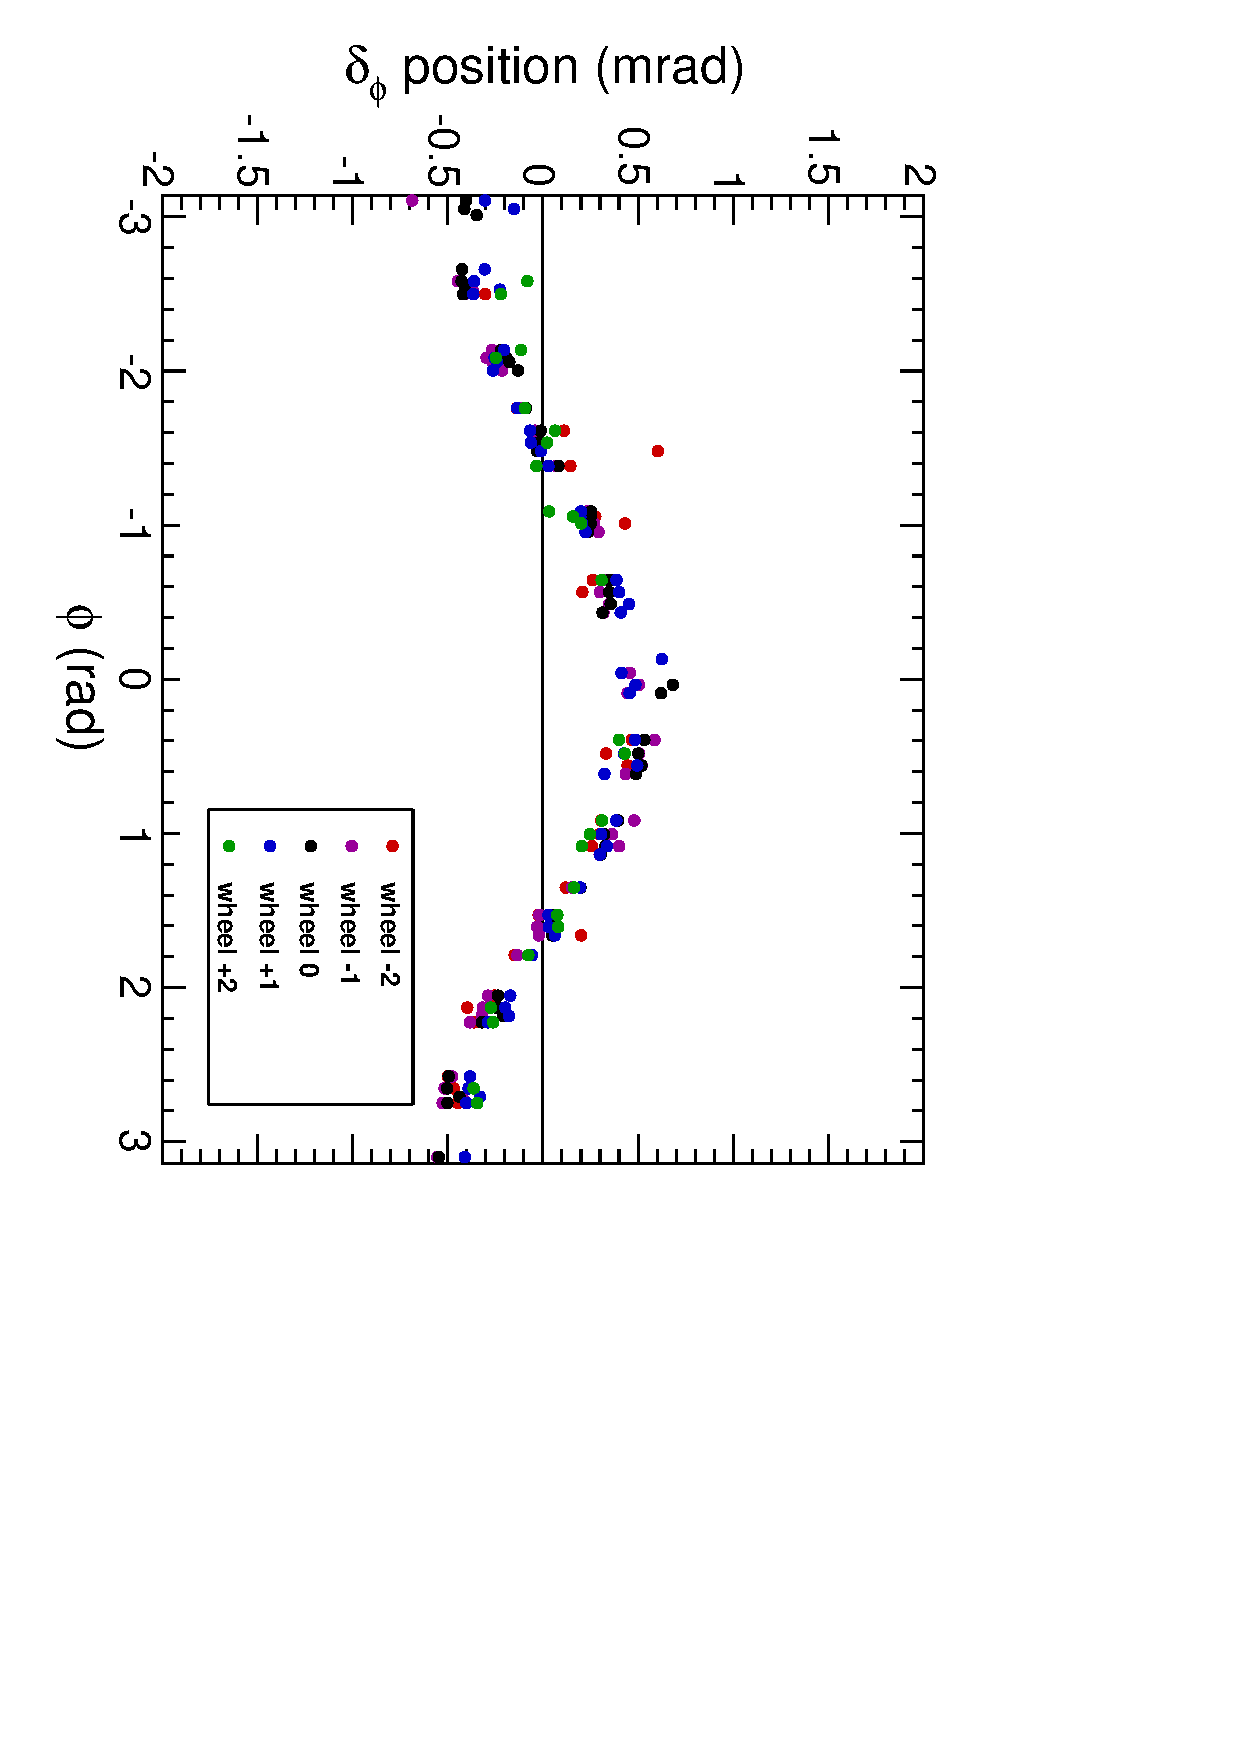
\includegraphics[height=0.5\linewidth, angle=90]{startup_phi_phi_redo.pdf}
\includegraphics[height=0.5\linewidth, angle=90]{systematic_phi_phi_redo.pdf}
\end{frame}


%% \begin{frame}
%% \frametitle{Outline}
%% \begin{itemize}\setlength{\itemsep}{0.75 cm}
%% \item 
%% \end{itemize}
%% %% \hspace{-0.83 cm} \textcolor{darkblue}{\Large Outline2}
%% \end{frame}

%% \section*{First section}
%% \begin{frame}
%% \begin{center}
%% \Huge \textcolor{blue}{First section}
%% \end{center}
%% \end{frame}

\begin{frame}
\frametitle{Conclusions}
\begin{itemize}
\item<1-> Muon chamber measurements are sensitive to some global distortions of the tracker
\begin{itemize}
\item $q/p_T$ is especially useful for characterizing tracker:
  independent of DT misalignment, propagation errors must be
  antisymmetric in $q$, and sensitivity grows with distance
\item avoid dependence on muon alignment by selecting only one
  alignable, ignore the simple trends that may be due to its own
  misalignment
\end{itemize}

\item<2-> The true shape of the tracker is probably something like sagitta
\begin{itemize}
\item tracker alignment with cosmics is insensitive to this mode
\item residuals distributions {\it most closely} resemble sagitta (of the 9)
\item MC misalignments also resemble sagitta (but also not exact)
\end{itemize}

\item<3-> This will likely be a long-term project
\begin{itemize}
\item first identify the pattern (possibly not unique), then cross-check data from other sources, like resonances
\item method for applying constraint: Markus's talk?
\item DT wire endpin measurements exist; can verify \mbox{DT layer rigidity\hspace{-1 cm}}
\item anyone interested?
\end{itemize}
\end{itemize}
\label{numpages}
\end{frame}

\end{document}
